%\documentclass[a4,semhelv,landscape]{seminar}
\documentclass[landscape]{slides}
%\documentclass[pdf, default, slideBW, nocolorBG]{prosper}
\usepackage[left=0.2cm,top=0.2cm,right=0.2cm,nohead,nofoot]{geometry}
%\def\everyslide{\sffamily}
%\usepackage{fullpage}
\usepackage{graphicx}
\usepackage[usenames]{color}
%\usepackage{color}
\usepackage{verbatim}
\usepackage{nopageno}
\usepackage{setspace}
%\usepackage{times}
% define some nice colors
\definecolor{myred}{rgb}{0.6,0,0}
\definecolor{myblue}{rgb}{0,0.2,0.4}
\definecolor{mygreen}{rgb}{0,0.5,0.0}
\definecolor{mypurple}{cmyk}{0.5,1.0,0.0,0.0}
%\color{myblue}

\begin{document}
%%%%%%%%%%%%%%%%%%%%%%%%%%%%%%%%%%%%%%%%%%%%%%%%%%%%%%%%%%%%%%%%%%%%
%Slide 0 - title
\begin{slide}
\begin{center}
\large{\textbf{Multiple alignment using sequence family profiles}}

\normalsize

Eric Nawrocki

Sean Eddy's Lab

\medskip

\medskip

\small

\begin{tabular}{c}
Howard Hughes Medical Institute \\ 
Janelia Farm Research Campus \\
\end{tabular}

\vspace{0.1in}


\includegraphics[width=2.5in]{figs/janelia-logo}
\end{center}
\end{slide}
%%%%%%%%%%%%%%%%%%%%%%%%%%%%%%%%%%%%%%%%%%%%%%%%%%%%%%%%%%%%%%%%%%%%%%
\begin{slide}
\begin{center}
\textbf{Small subunit ribosomal RNA and the tree of life}
\end{center}
\medskip
\begin{minipage}{5.2in}
\small

\begin{itemize}
\item 1977 - Carl Woese decided to classify all living things phylogenetically
\item needed ``\emph{a molecule of appropriately broad distribution}'' for comparative analysis
\item SSU rRNA was chosen
\begin{itemize}
  \item universally distributed
  \item highly conserved 
  \item large enough to provide sufficient data (1500-1800 nt)
  \item readily isolated
\end{itemize}
\end{itemize}

\vspace{2.7in}
\end{minipage}
\hspace{0.1in}
\begin{minipage}{5.5in}
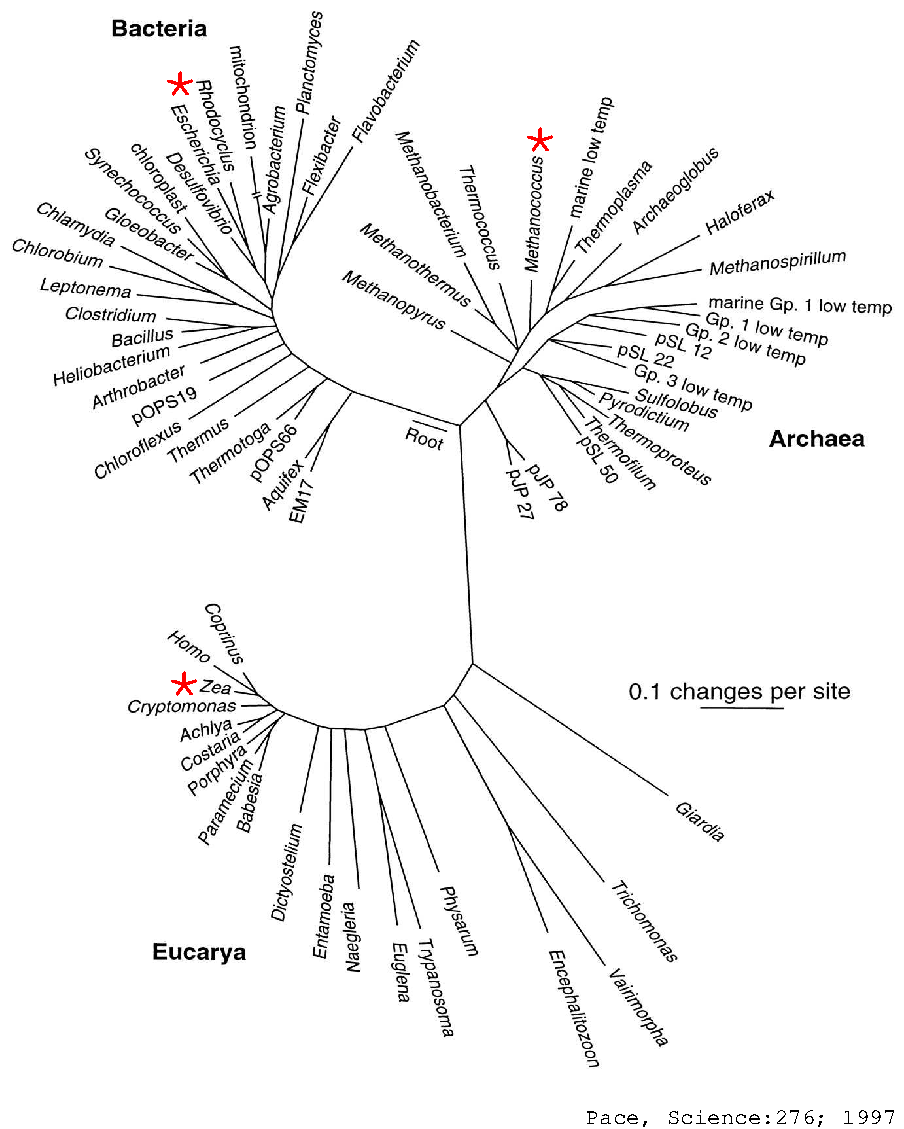
\includegraphics[width=5.5in]{figs/bigtol}
\end{minipage}  
\end{slide}
%%%%%%%%%%%%%%%%%%%%%%%%%%%%%%%%%%%%%%%%%%%%%%%%%%%%%%%%%%%%%%%%%%%%%%%%%%
\begin{slide}
\begin{center}

\textbf{Universal conservation of SSU rRNA}
\end{center}
\vspace{0.5in}
\small
\hspace{0.75in}
\emph{Escherichia coli}
\hspace{1.2in}
\emph{Methanococcus vannielii}
\hspace{1.2in}
\emph{Zea mays}

\begin{center}
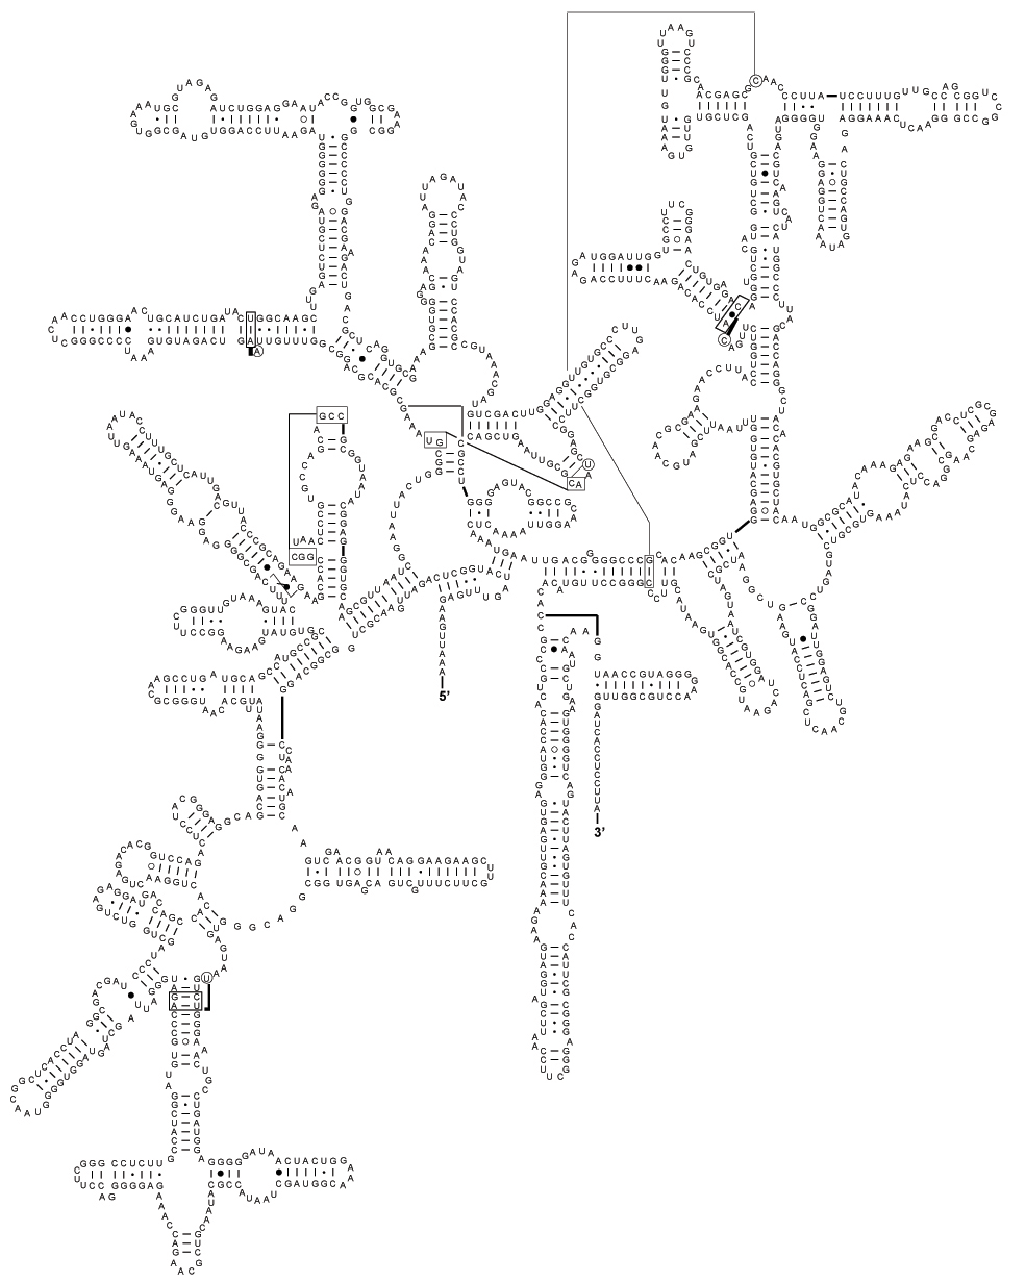
\includegraphics[height=4.45in]{figs/ecoli_16S_man}
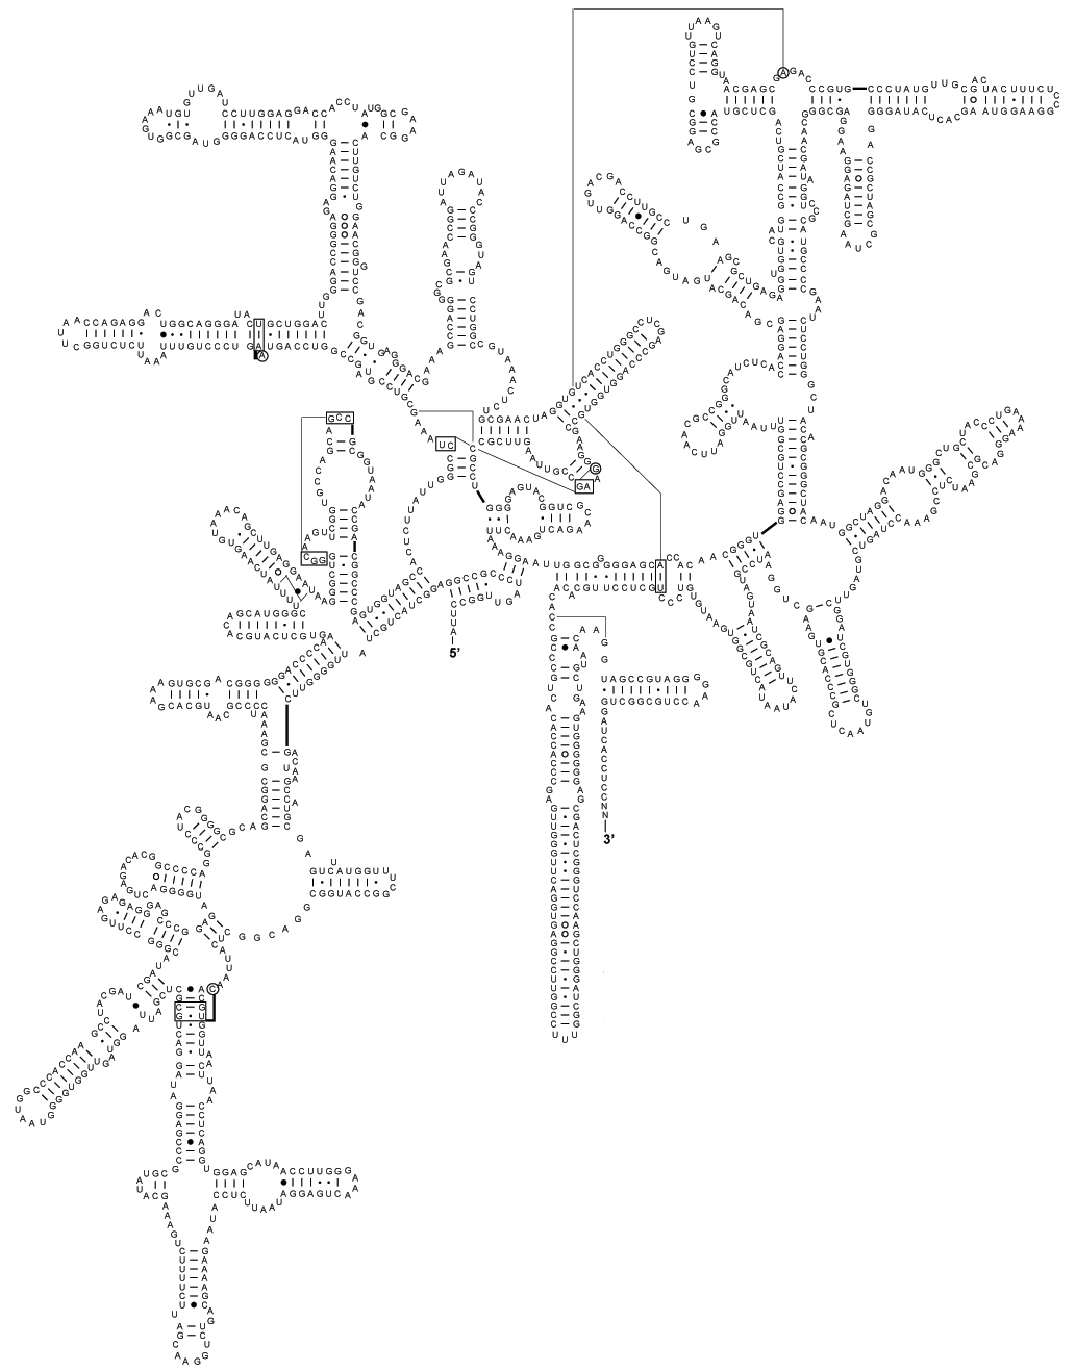
\includegraphics[height=4.45in]{figs/mvan_16S_man}
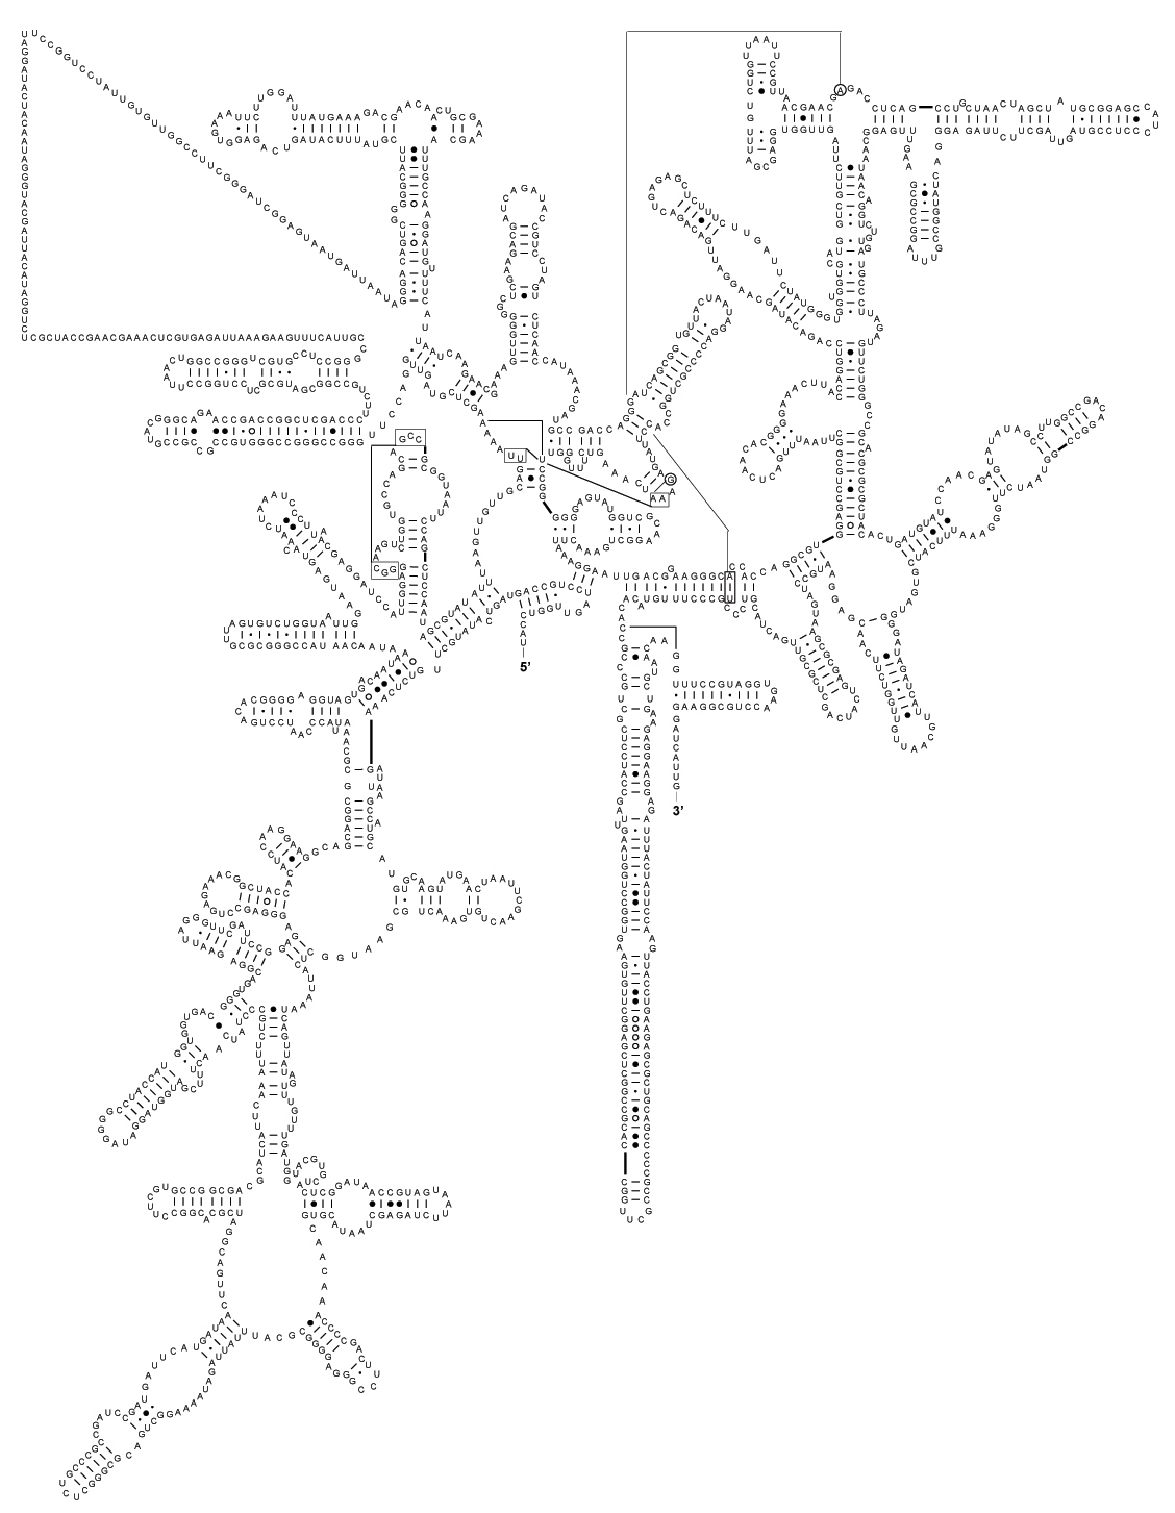
\includegraphics[height=4.45in]{figs/zmays_16S_man}
\end{center}

\begin{flushright}
\tiny{\texttt{Secondary structure diagrams from:}} \\
\tiny{\texttt{URL:http://www.rna.ccbb.utexas.edu/}}
\end{flushright}
\vfill
\end{slide}
%%%%%%%%%%%%%%%%%%%%%%%%%%%%%%%%%%%%%%%%%%%%%%%%%%%%%%%%%%%%%%%%%%%%%%%%%%
%%%%%%%%%%%%%%%%%%%%%%%%%%%%%%%%%%%%%%%%%%%%%%%%%%%%%%%%%%%%%%%%%%%%%%%%%%
%%%%%%%%%%%%%%%%%%%%%%%%%%%%%%%%%%%%%%%%%%%%%%%%%%%%%%%%%%%%%%%%%%%%%%%%%%
%%%%%%%%%%%%%%COMMENTED OUT%%%%%%%%%%%%%%%%%%%%%%%%%%%%%%%%%%%%%%%%%%%%%%%
\begin{comment}
\begin{slide}
\begin{center}
\textbf{Sequence conservation in SSU rRNA}
\end{center}
\vspace{0.5in}
\small
\hspace{1.5in}
\underline{bacteria}
\hspace{2.2in}
\underline{archaea}
\hspace{2.2in}
\underline{eukarya}

\begin{center}
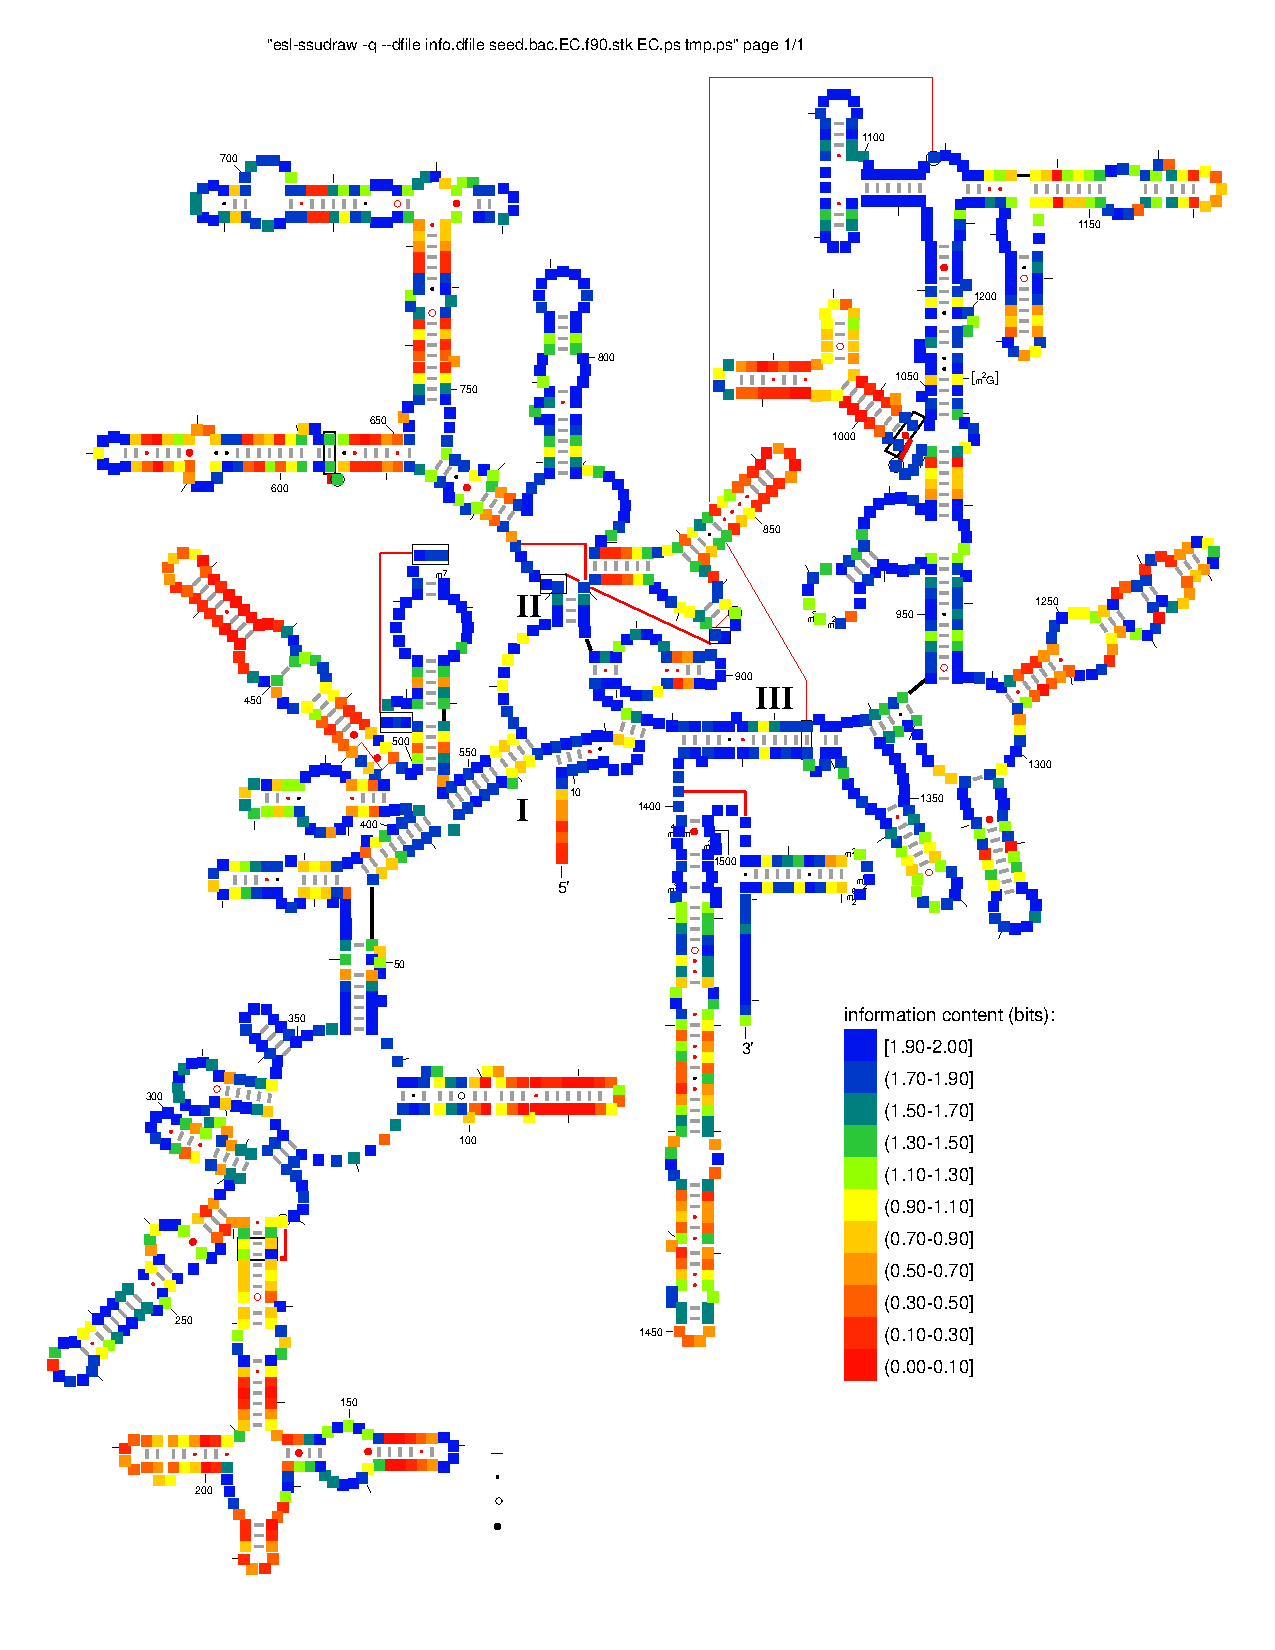
\includegraphics[height=4.45in]{figs/bac_info_heat}
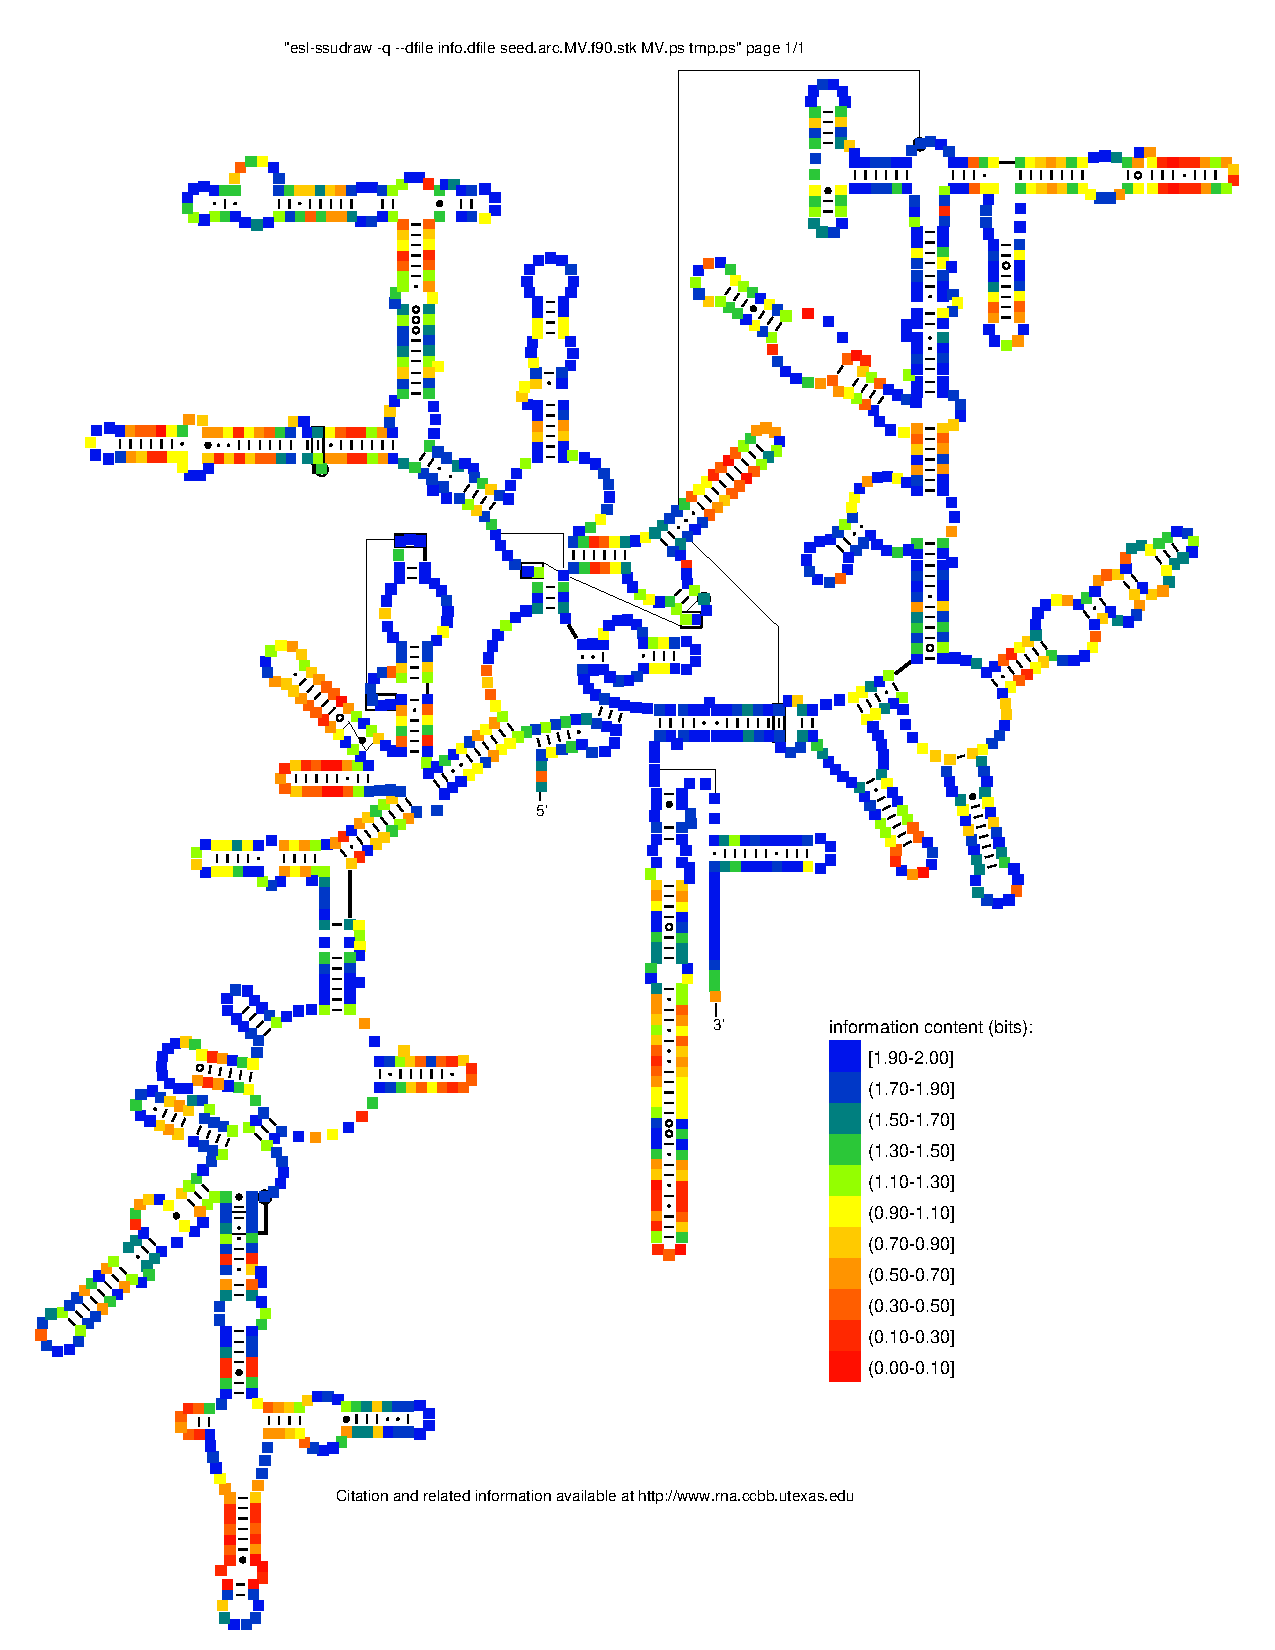
\includegraphics[height=4.45in]{figs/arc_info_heat}
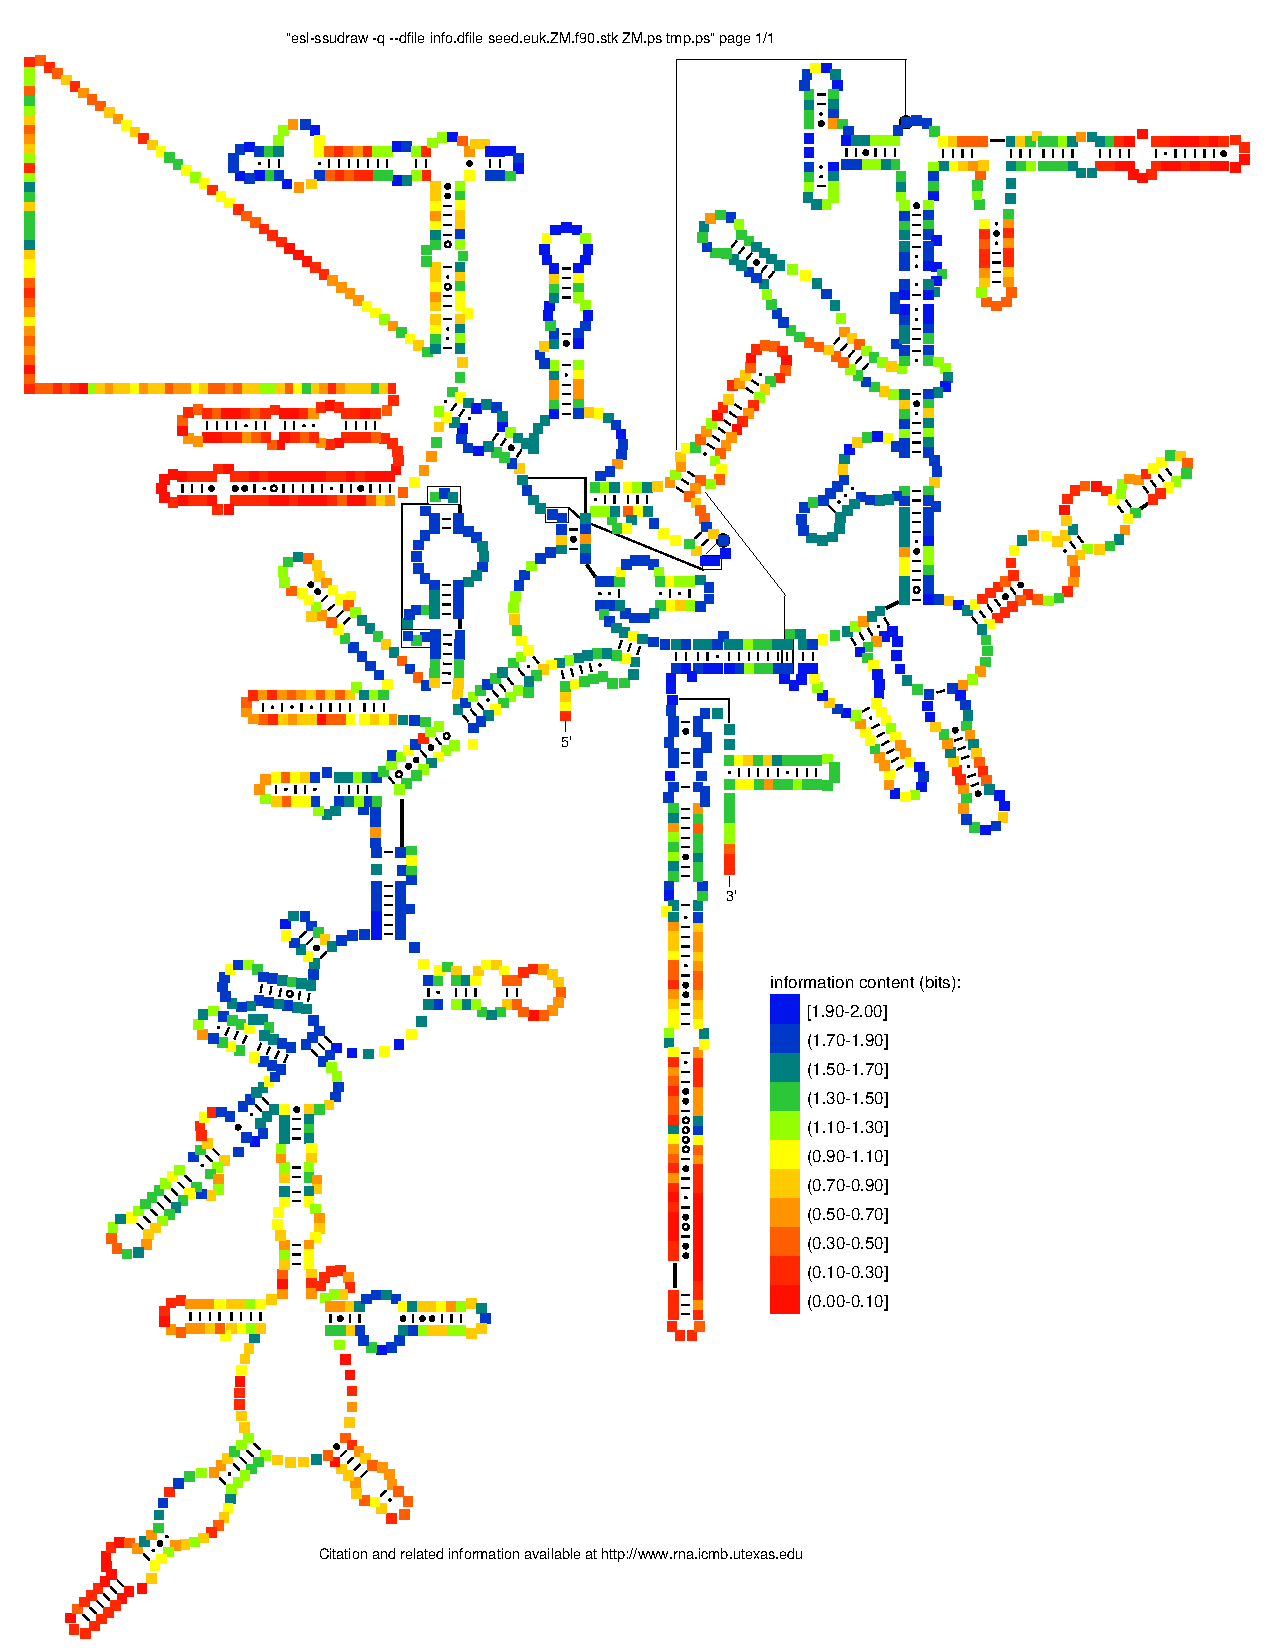
\includegraphics[height=4.45in]{figs/euk_info_heat}
\end{center}

\begin{flushright}
\tiny{\texttt{Secondary structure diagrams created based}} \\
\tiny{\texttt{alignments and diagrams from:}} \\
\tiny{\texttt{URL:http://www.rna.ccbb.utexas.edu/}}
\end{flushright}
\vfill
\end{slide}
\end{comment}
%%%%%%%%%%%%%COMMENTED OUT%%%%%%%%%%%%%%%%%%%%%%%%%%%%%%%%%%%%%%%%%%%%%%%%
%%%%%%%%%%%%%%%%%%%%%%%%%%%%%%%%%%%%%%%%%%%%%%%%%%%%%%%%%%%%%%%%%%%%%%%%%%
%%%%%%%%%%%%%%%%%%%%%%%%%%%%%%%%%%%%%%%%%%%%%%%%%%%%%%%%%%%%%%%%%%%%%%%%%%
%%%%%%%%%%%%%%%%%%%%%%%%%%%%%%%%%%%%%%%%%%%%%%%%%%%%%%%%%%%%%%%%%%%%%%%%%%
\begin{slide}
\begin{center}

\textbf{Environmental surveys target SSU}
\end{center}
\medskip
\begin{minipage}{7in}
\small
\begin{itemize}
\item mid 1980s - Norman Pace develops methodology for determination
      of SSU sequences without cultivation
\item many different environments have been surveyed
\item known biodiversity has been greatly expanded:

\begin{itemize}
\item
  recognized bacterial phyla: \\
  11 in 1987, 36 in 1998, 52 in 2003, 67 in 2006...
\end{itemize}

\item SSU databases contain millions of sequences:
\begin{center}
\begin{tabular}{lrr}
  name & \# seqs & \# citations \\ \hline
  Silva & 3.2M & 1125 \\ 
  RDP   & 2.6M & 1170 \\
  Greengenes & 1.0M & 1012 \\
\end{tabular}
\end{center}
\end{itemize}

\tiny
Silva: Pruesse et al., 2007 NAR 35.21:7188-96 \\
RDP: Cole et al., 2009 NAR 37:D141-45 \\
Greengenes: DeSantis et al., 2006 AEM 72:5069-72 \\

\vspace{1.6in}
\end{minipage}
\hspace{0.1in}
\begin{minipage}{3in}
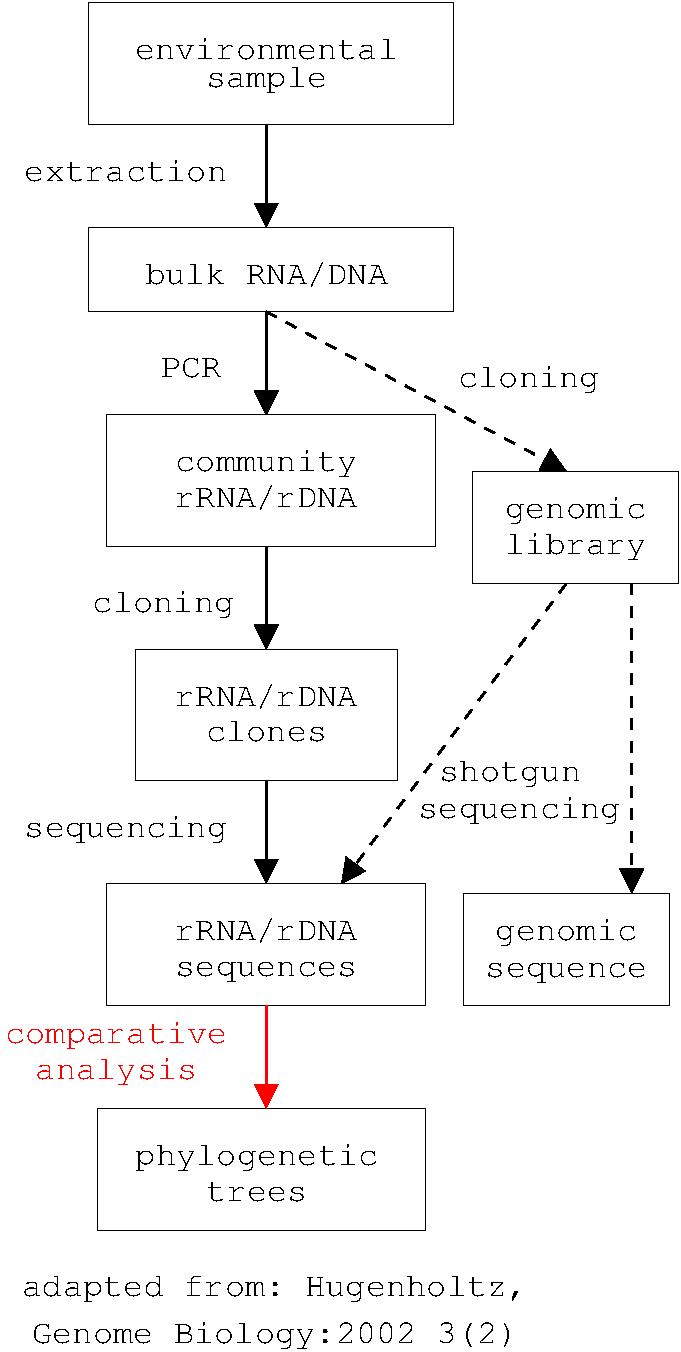
\includegraphics[height=6in]{figs/environmental}
\vspace{1in}
\end{minipage}
\end{slide}

%%%%%%%%%%%%%%%%%%%%%%%%%%%%%%%%%%%%%%%%%%%%%%%%%%%%%%%%%%%%%%%%%%%%%%%%%%
\begin{slide}
\begin{center}

%\large
\textbf{The comparative analysis step: \\ \textcolor{red}{Alignment} and Phylogenetic Inference}
\end{center}

\center{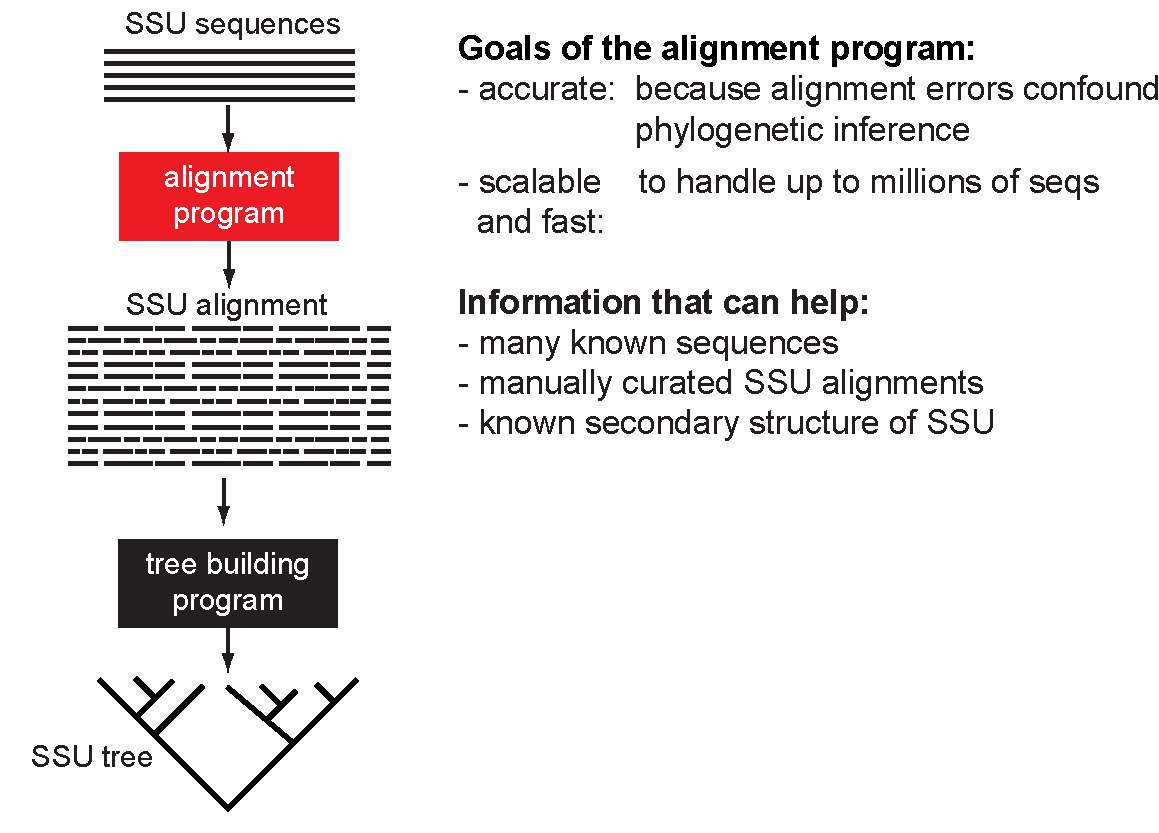
\includegraphics[height=7in]{figs/seq2tree-2013-goals}}
%\center{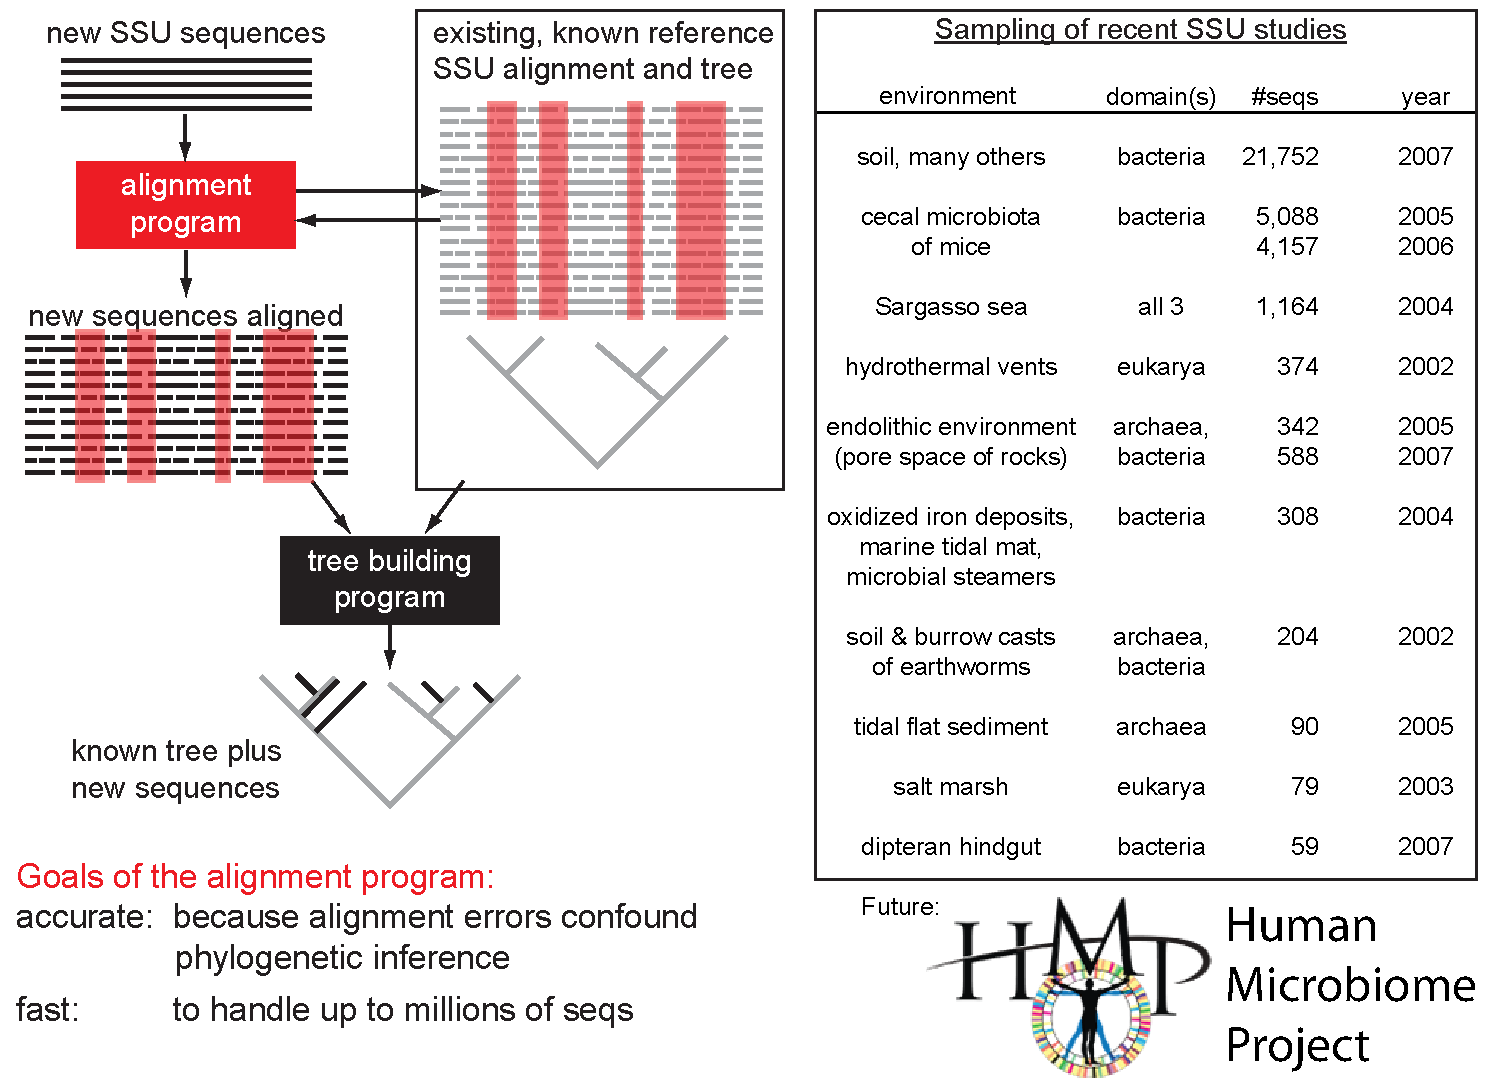
\includegraphics[height=7in]{figs/ssu_list_and_seq2tree_masked}}
\vfill
\end{slide}
%%%%%%%%%%%%%%%%%%%%%%%%%%%%%%%%%%%%%%%%%%%%%%%%%%%%%%%%%%%%%%%%%%%%%%%%%%
\begin{slide}
\begin{center}
\emph{De novo} \textbf{multiple sequence alignment methods assume very little}
\end{center}

\center{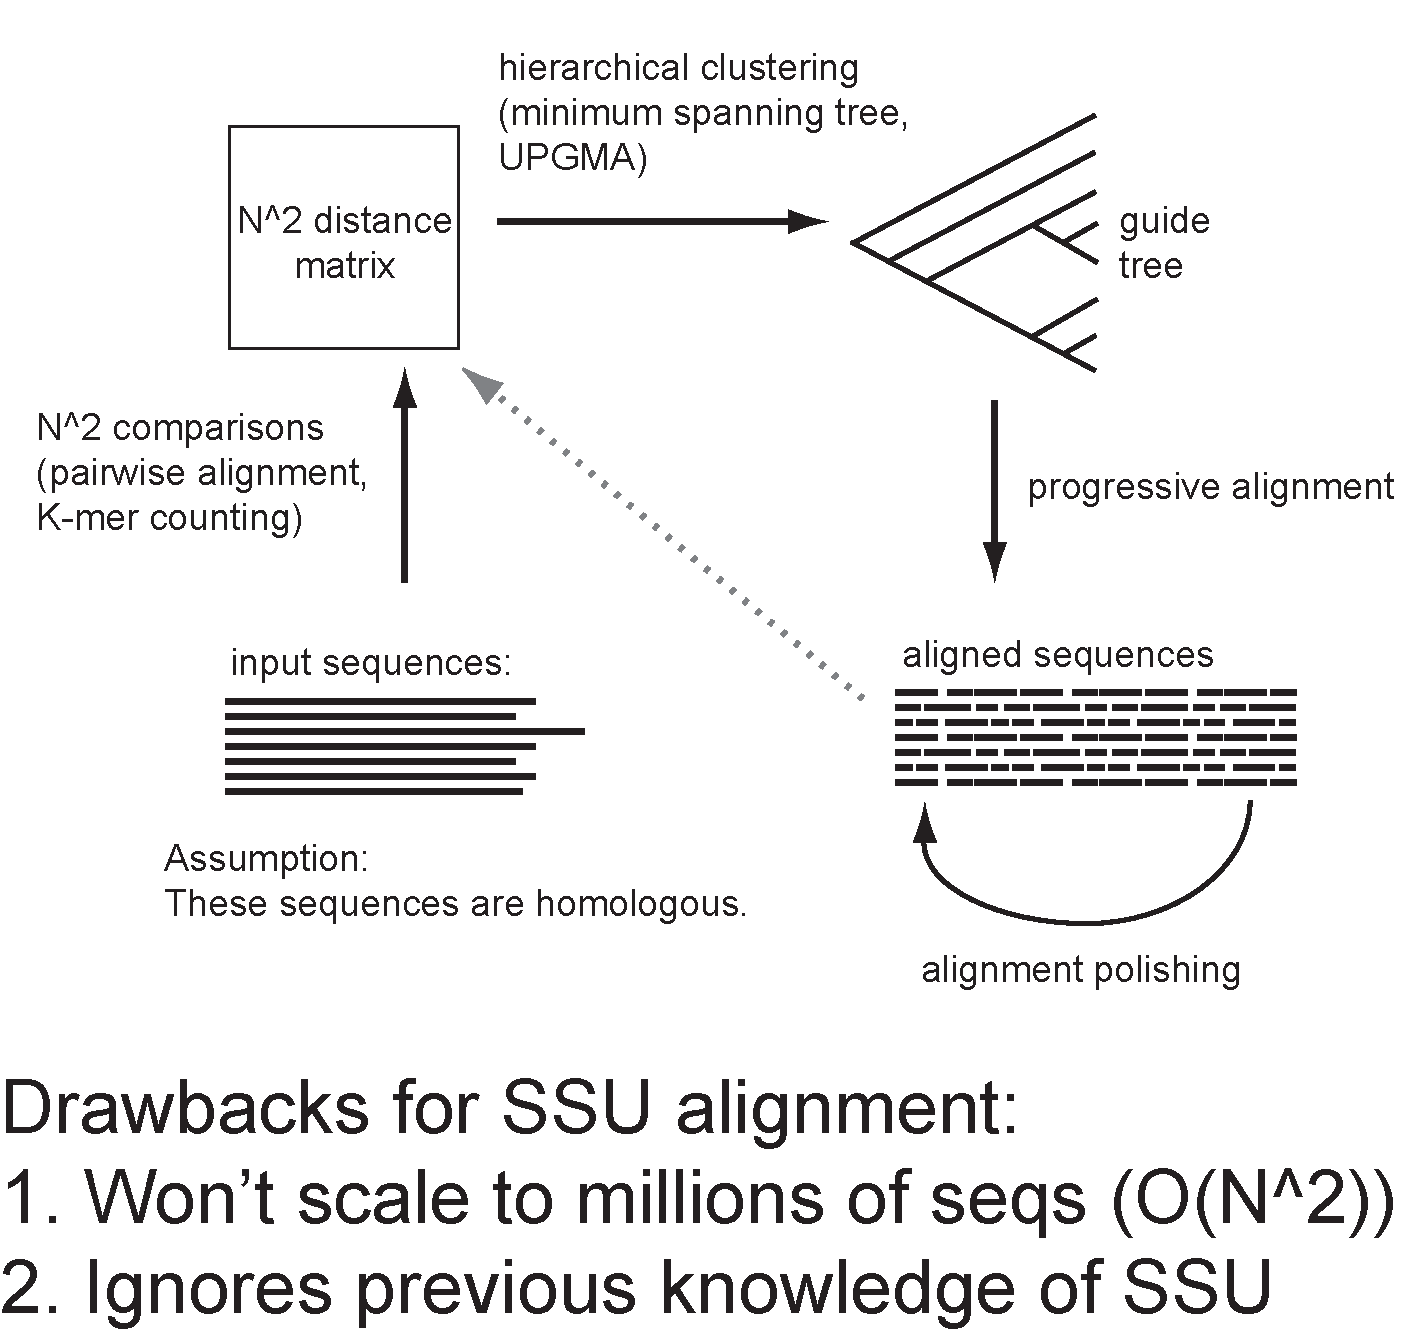
\includegraphics[height=7in]{figs/denovo-alignment}}

\vfill
\end{slide}
%%%%%%%%%%%%%%%%%%%%%%%%%%%%%%%%%%%%%%%%%%%%%%%%%%%%%%%%%%%%%%%%%%%%
\begin{slide}
\begin{center}
\textbf{A trusted (probably manually curated) reference alignment can help}
\end{center}

\center{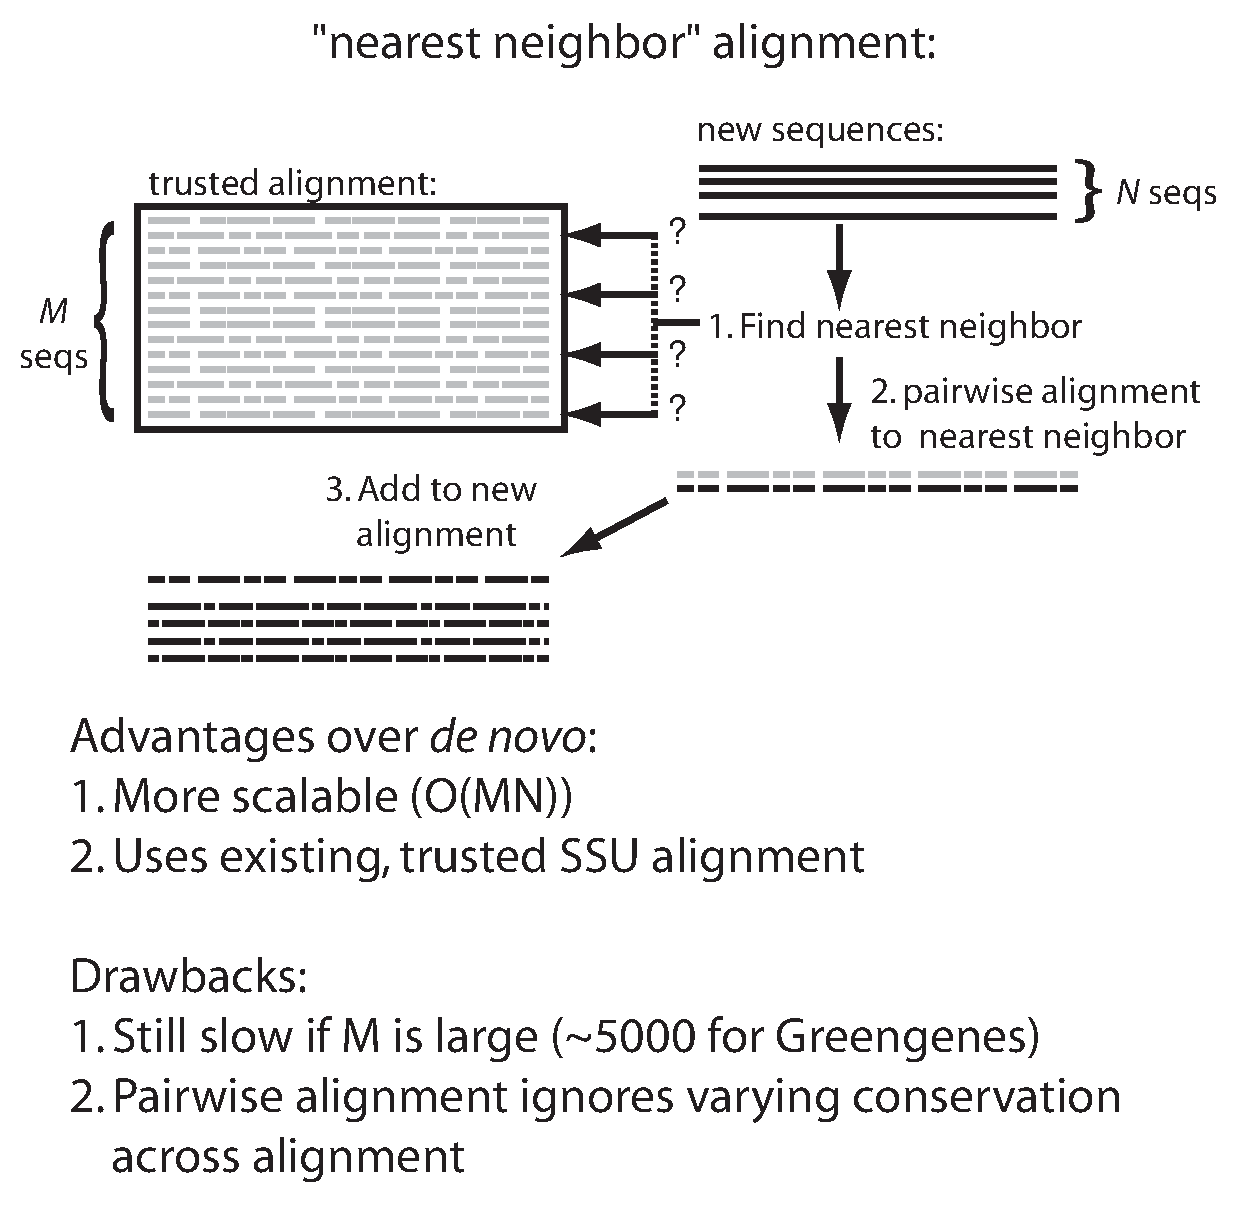
\includegraphics[height=7in]{figs/nn-only}}

\vfill
\end{slide}
%%%%%%%%%%%%%%%%%%%%%%%%%%%%%%%%%%%%%%%%%%%%%%%%%%%%%%%%%%%%%%%%%%%%
\begin{slide}
\begin{center}
\textbf{Profile-based alignment is $O(N)$}
\end{center}

%\center{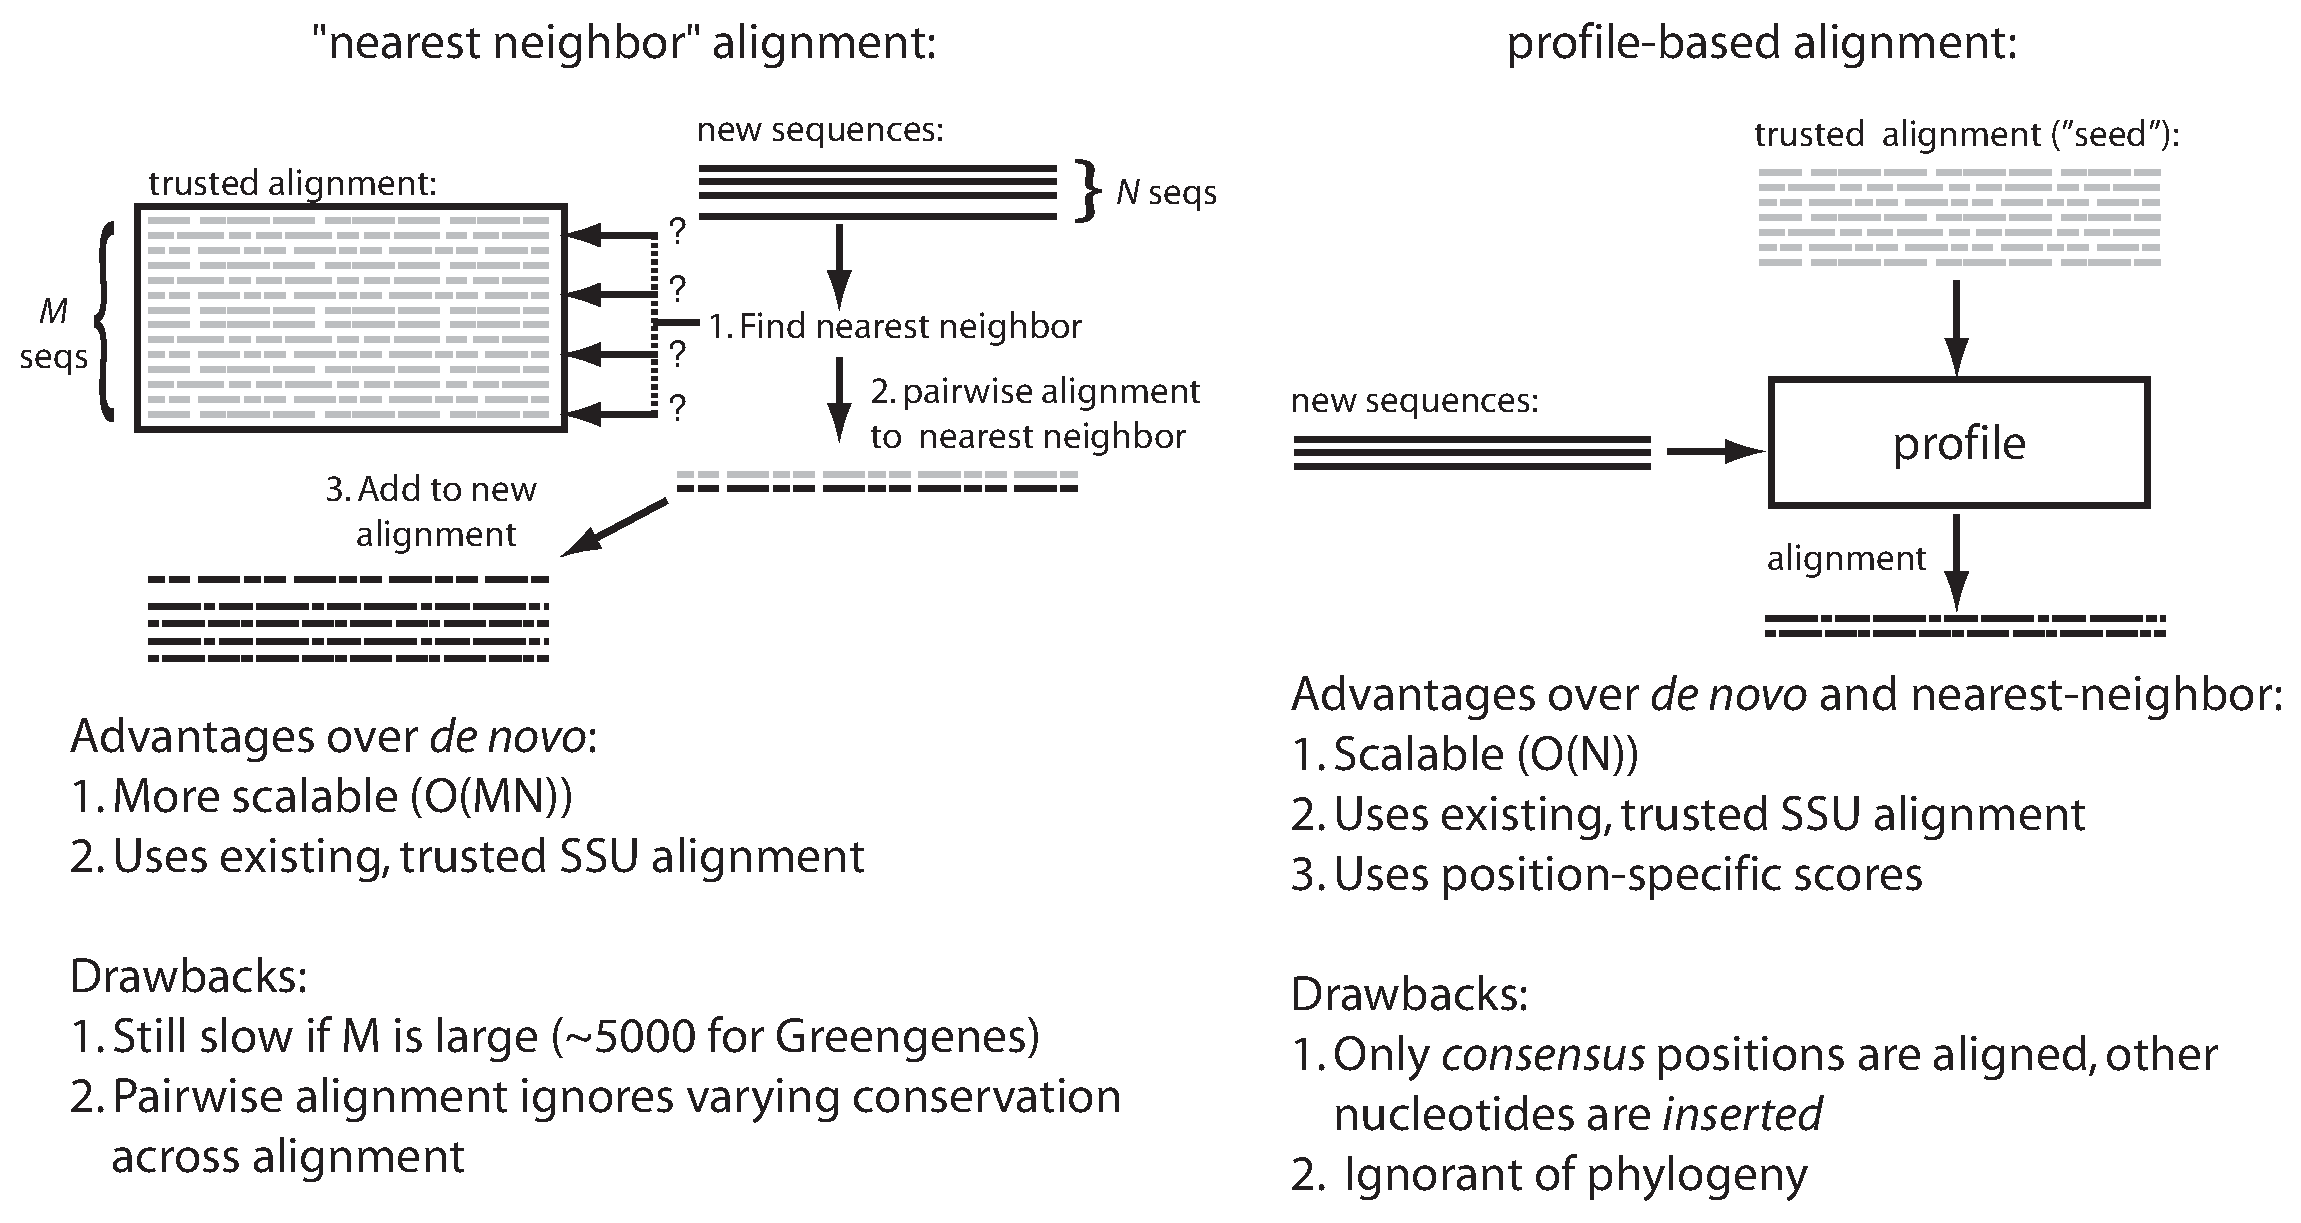
\includegraphics[width=10in]{figs/nn-v-profile}}
\center{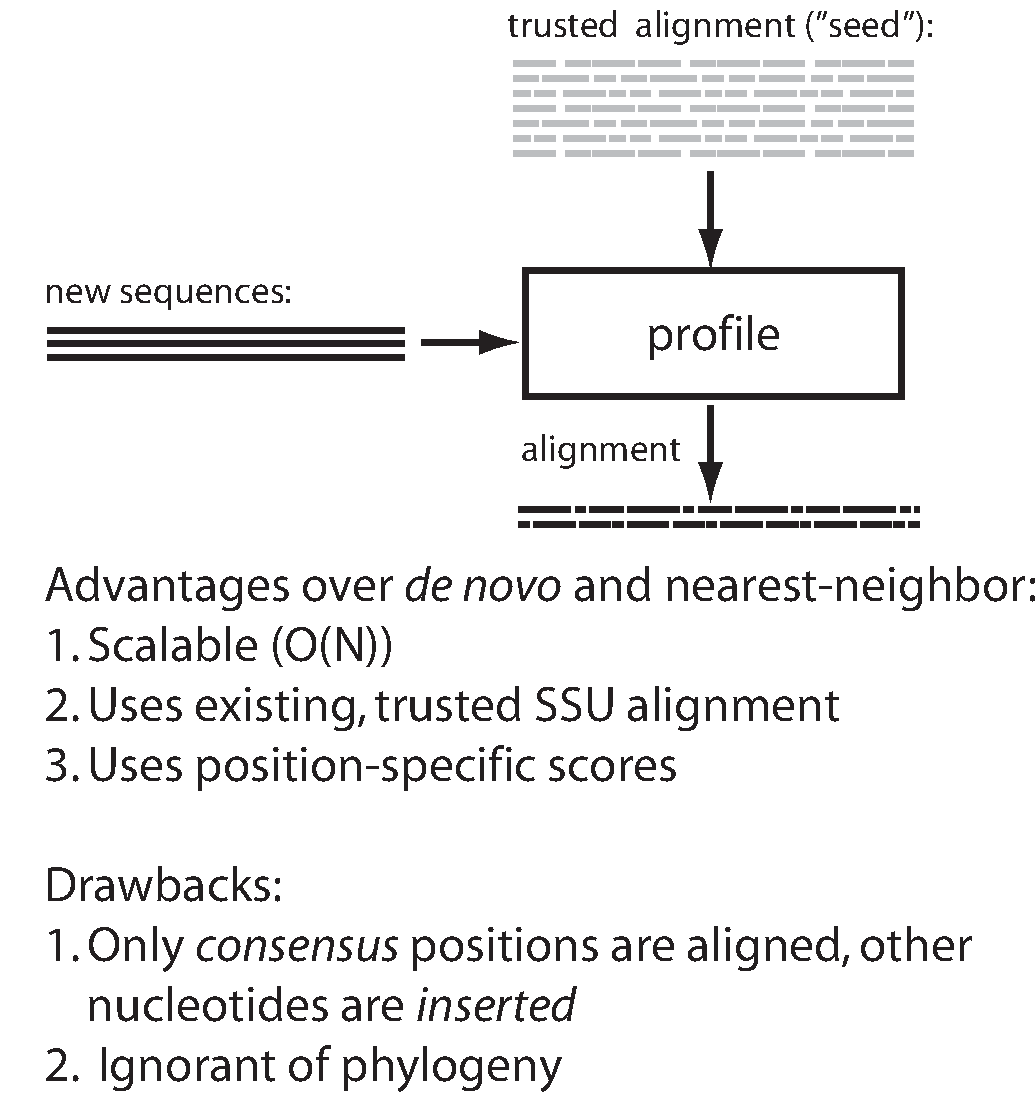
\includegraphics[height=7in]{figs/profile-only}}

\vfill
\end{slide}
%%%%%%%%%%%%%%%%%%%%%%%%%%%%%%%%%%%%%%%%%%%%%%%%%%%%%%%%%%%%%%%%%%%%
\begin{slide}
\begin{center}
\textbf{Profiles have position-specific scores \\ (substitutions, gap
    open, gap extend)}
\end{center}

\center{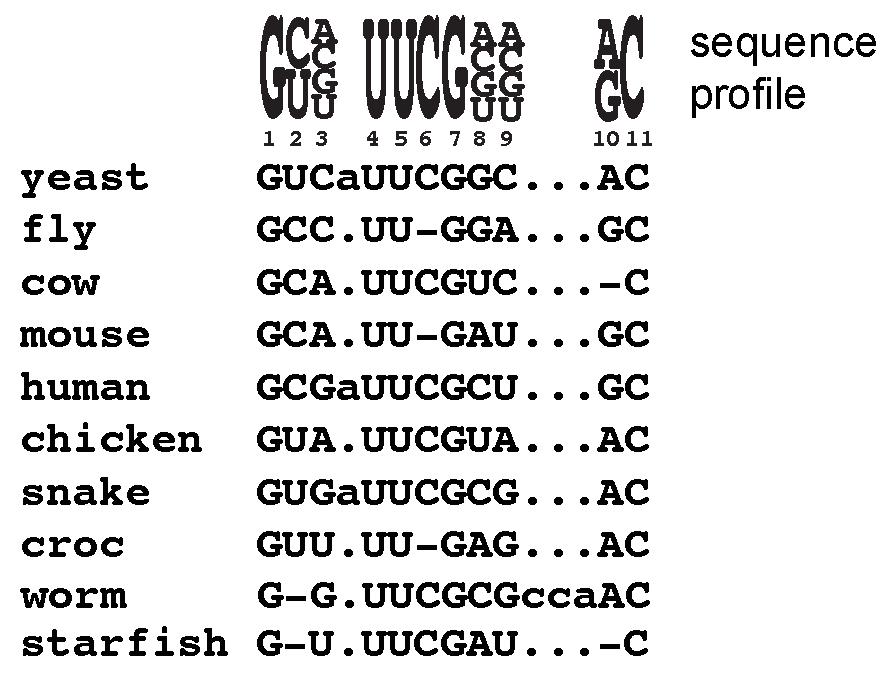
\includegraphics[height=6in]{figs/alignment-hmm-only}}

\vfill
\end{slide}
%%%%%%%%%%%%%%%%%%%%%%%%%%%%%%%%%%%%%%%%%%%%%%%%%%%%%%%%%%%%%%%%%%%%
\begin{slide}
\begin{center}
\textbf{Profiles HMMs are probabilistic profiles built from alignments}
\end{center}

\center{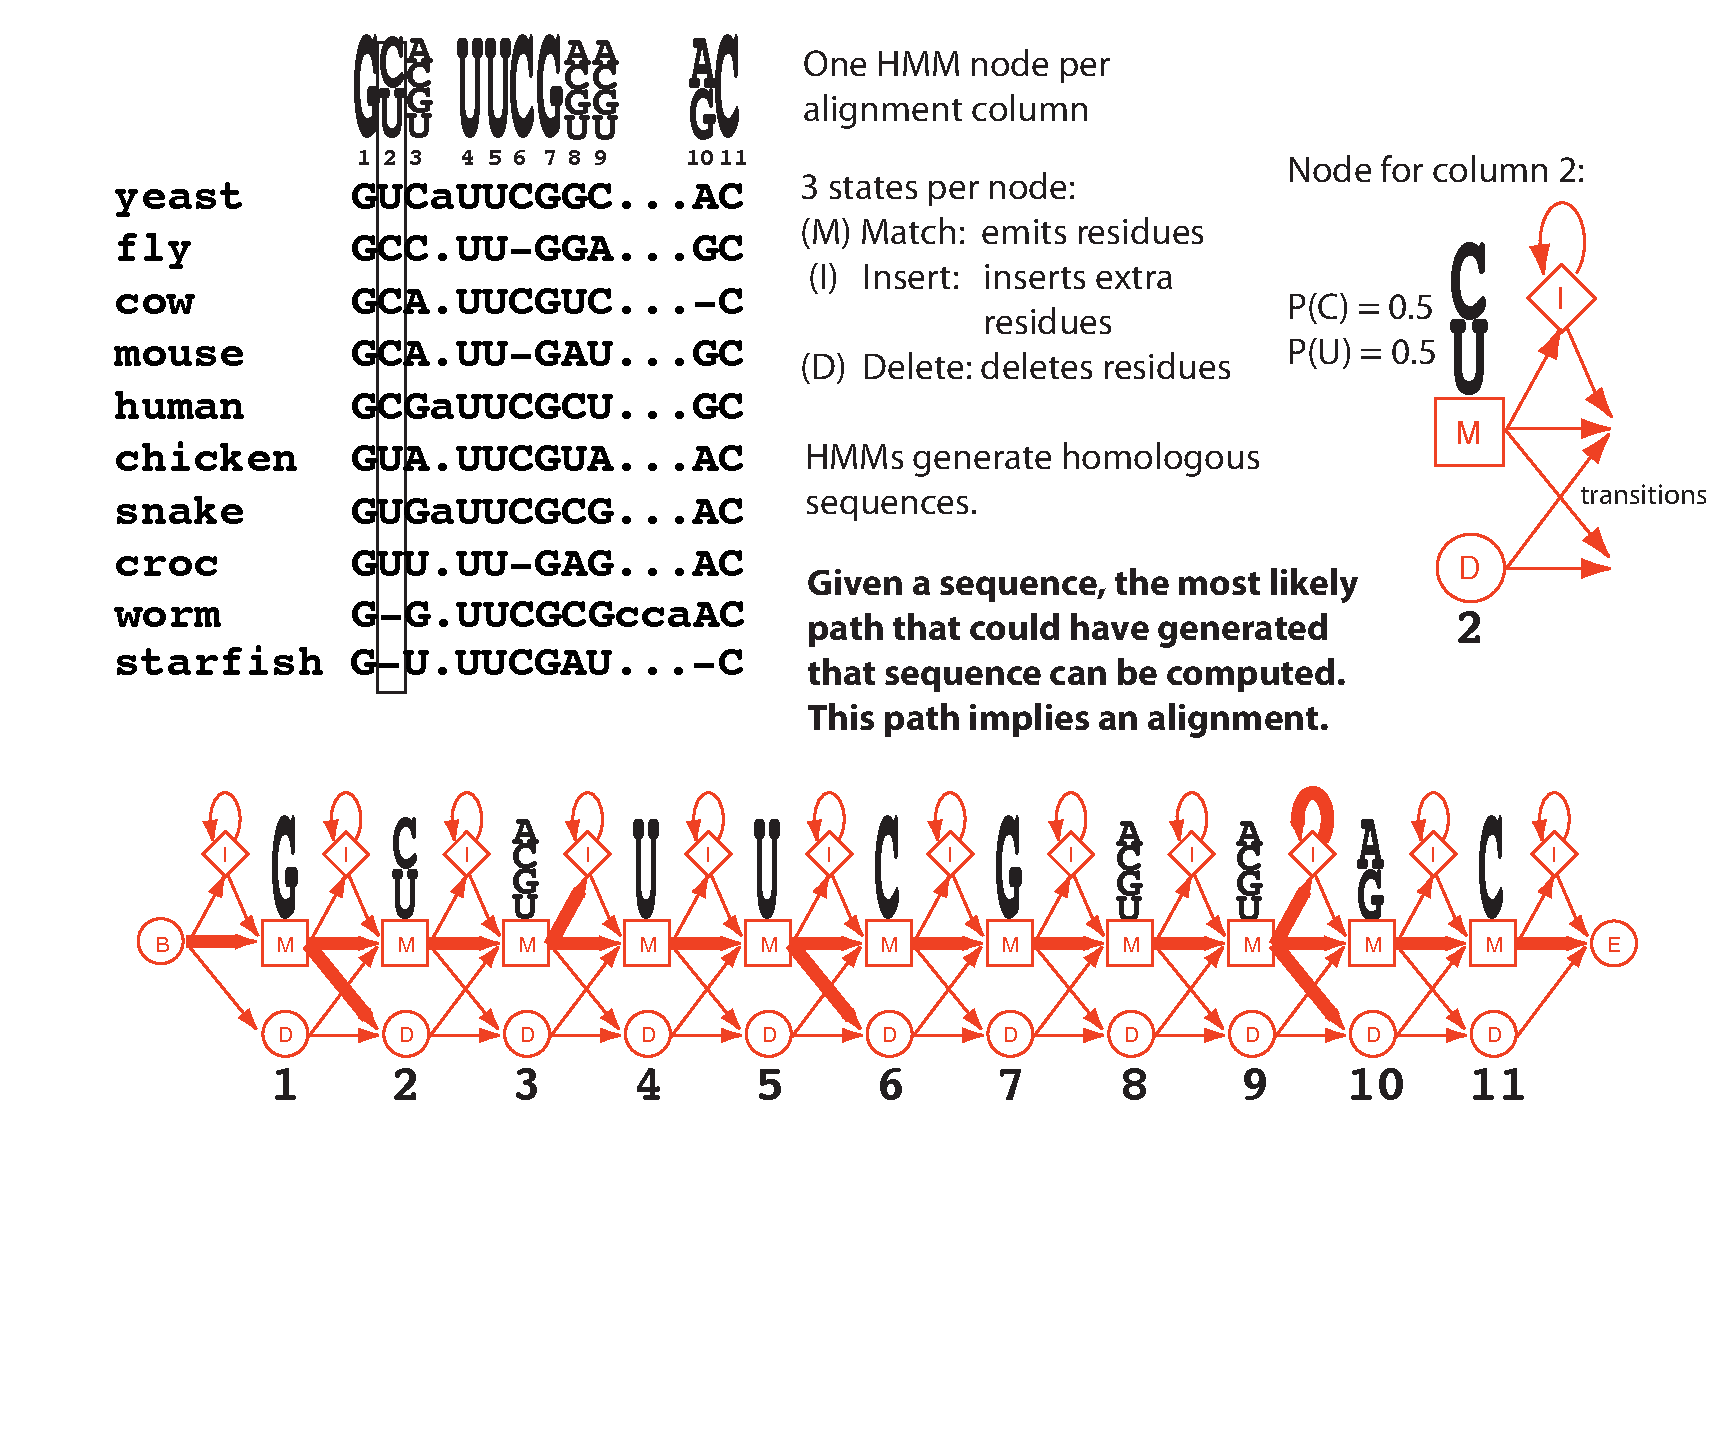
\includegraphics[height=7in]{figs/alignment-hmm-layer1}}

\vfill
\end{slide}
%%%%%%%%%%%%%%%%%%%%%%%%%%%%%%%%%%%%%%%%%%%%%%%%%%%%%%%%%%%%%%%%%%%%
\begin{slide}
\begin{center}
\textbf{Sequences are aligned to profiles HMMs using dynamic
  programming algorithms very similar to Smith-Waterman}
\end{center}

\center{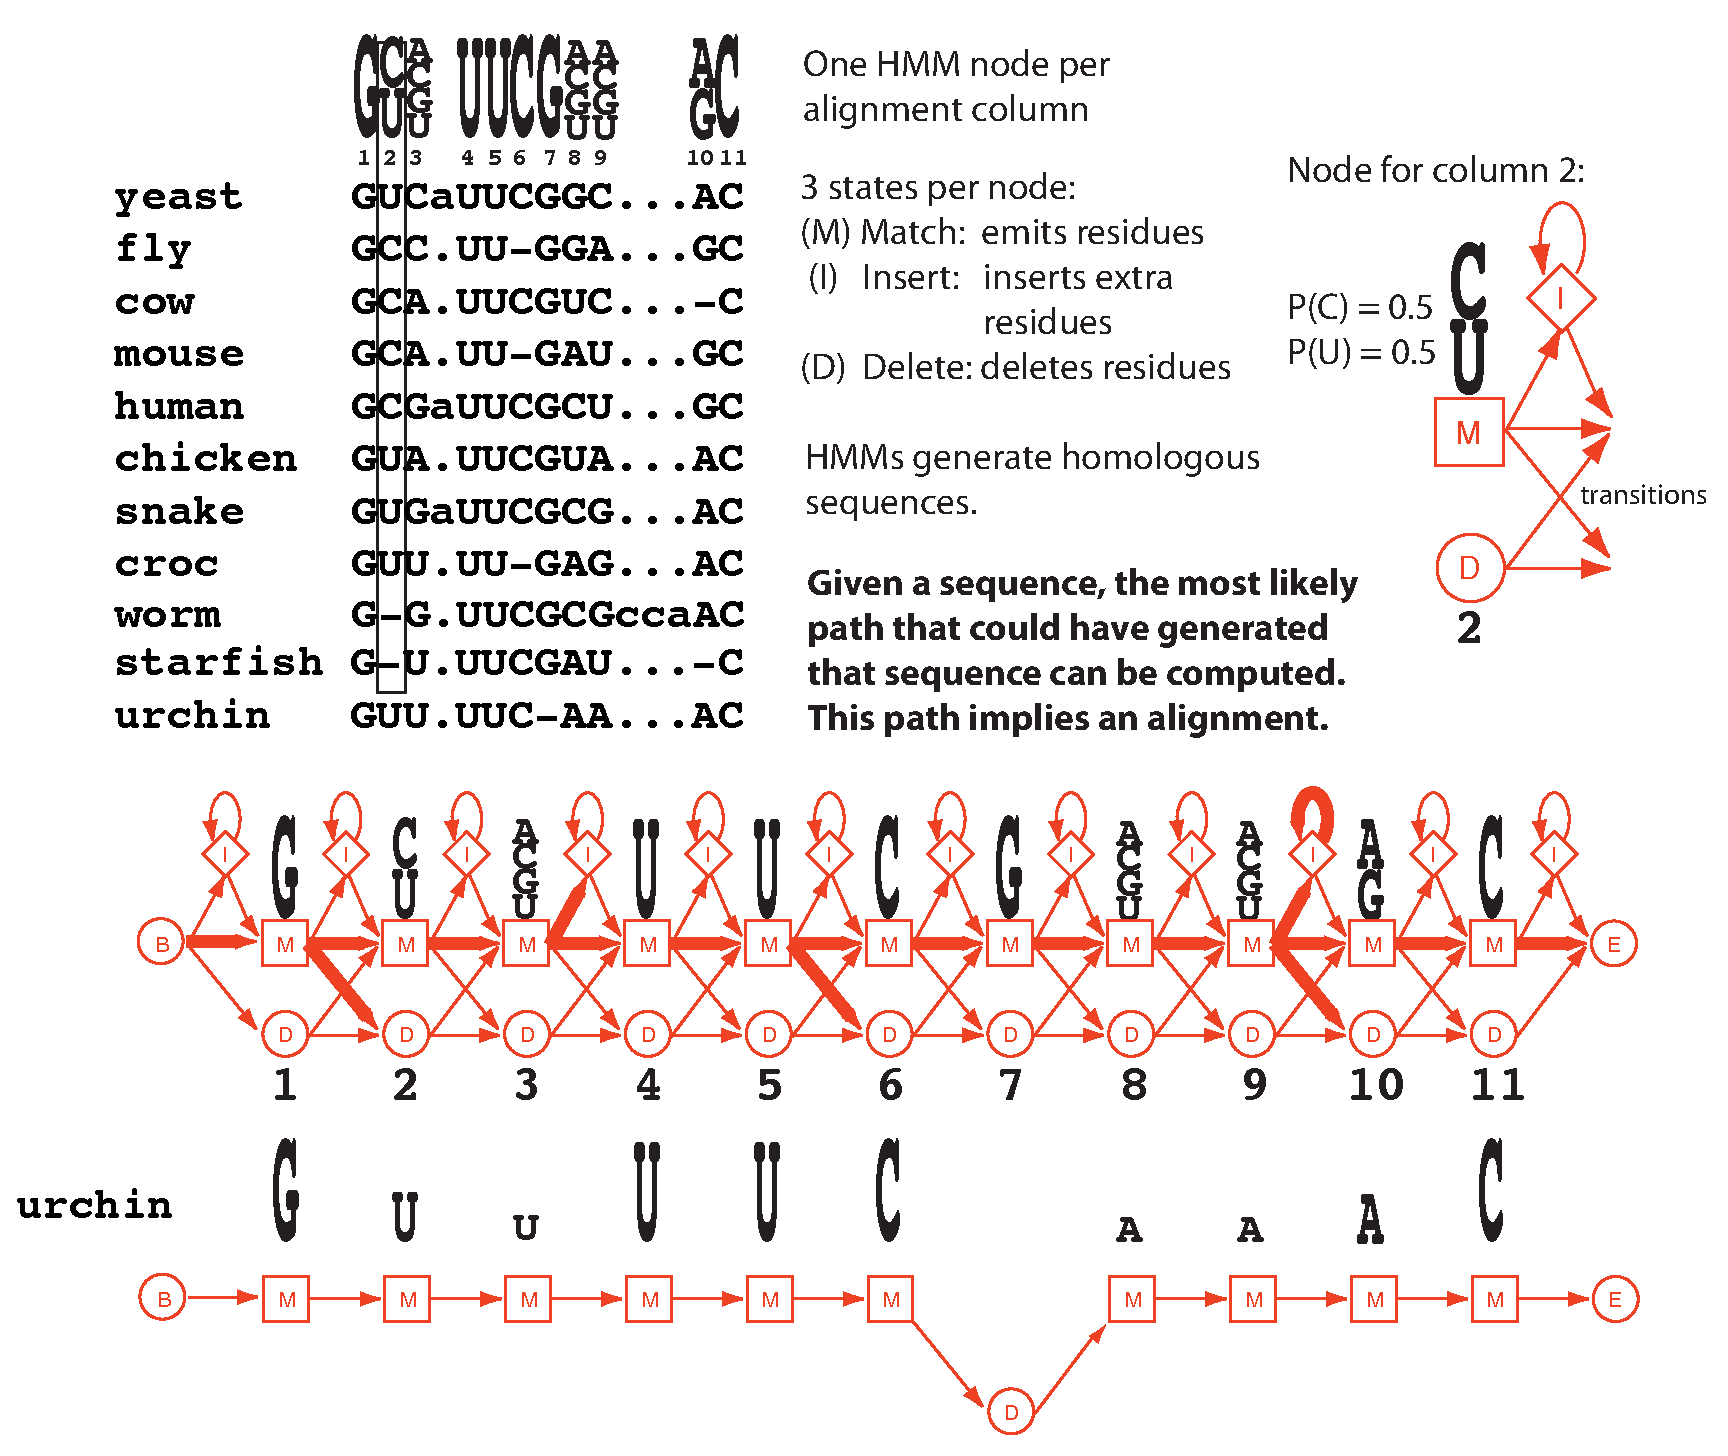
\includegraphics[height=7in]{figs/alignment-hmm-layer2}}

\vfill
\end{slide}
%%%%%%%%%%%%%%%%%%%%%%%%%%%%%%%%%%%%%%%%%%%%%%%%%%%%%%%%%%%%%%%%%%%%
\begin{slide}
\begin{center}
\textbf{Profile alignment can differ from pairwise alignment}
\end{center}

\center{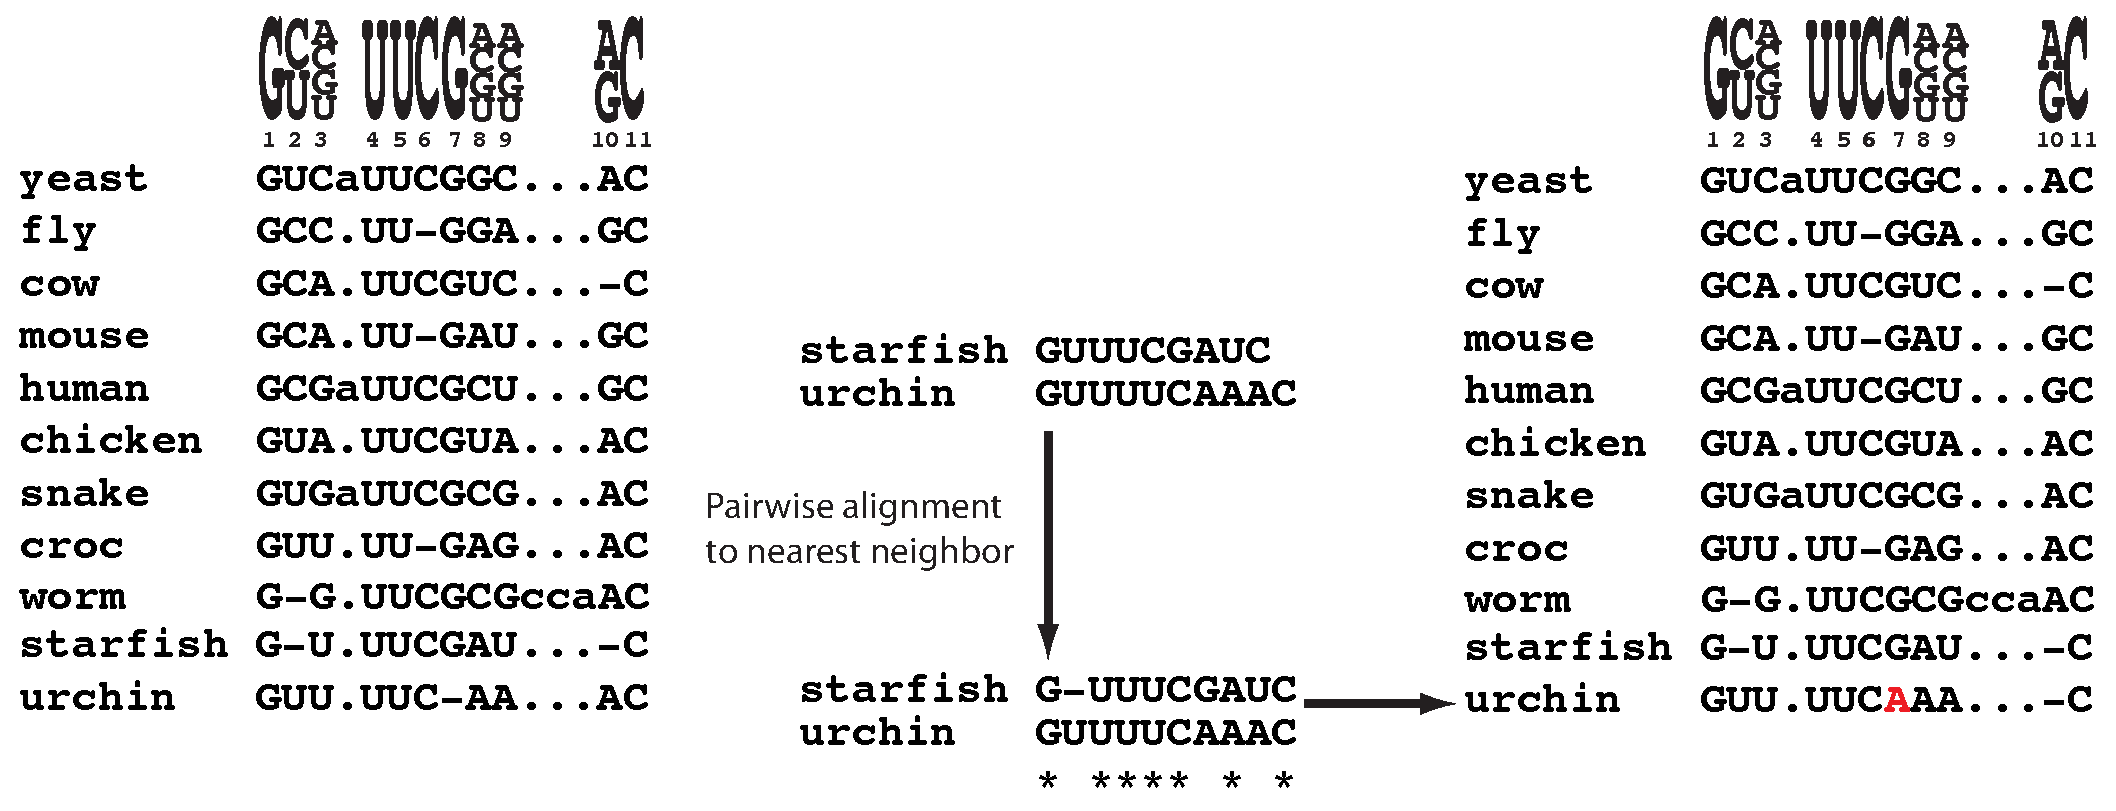
\includegraphics[width=10in]{figs/alignment-hmm-urchin-example}}

\vfill
\end{slide}
%%%%%%%%%%%%%%%%%%%%%%%%%%%%%%%%%%%%%%%%%%%%%%%%%%%%%%%%%%%%%%%%%%%%
\begin{slide}
%\begin{center}
%\center{\textbf{Bacterial SSU rRNA}}
%\end{center}
\center{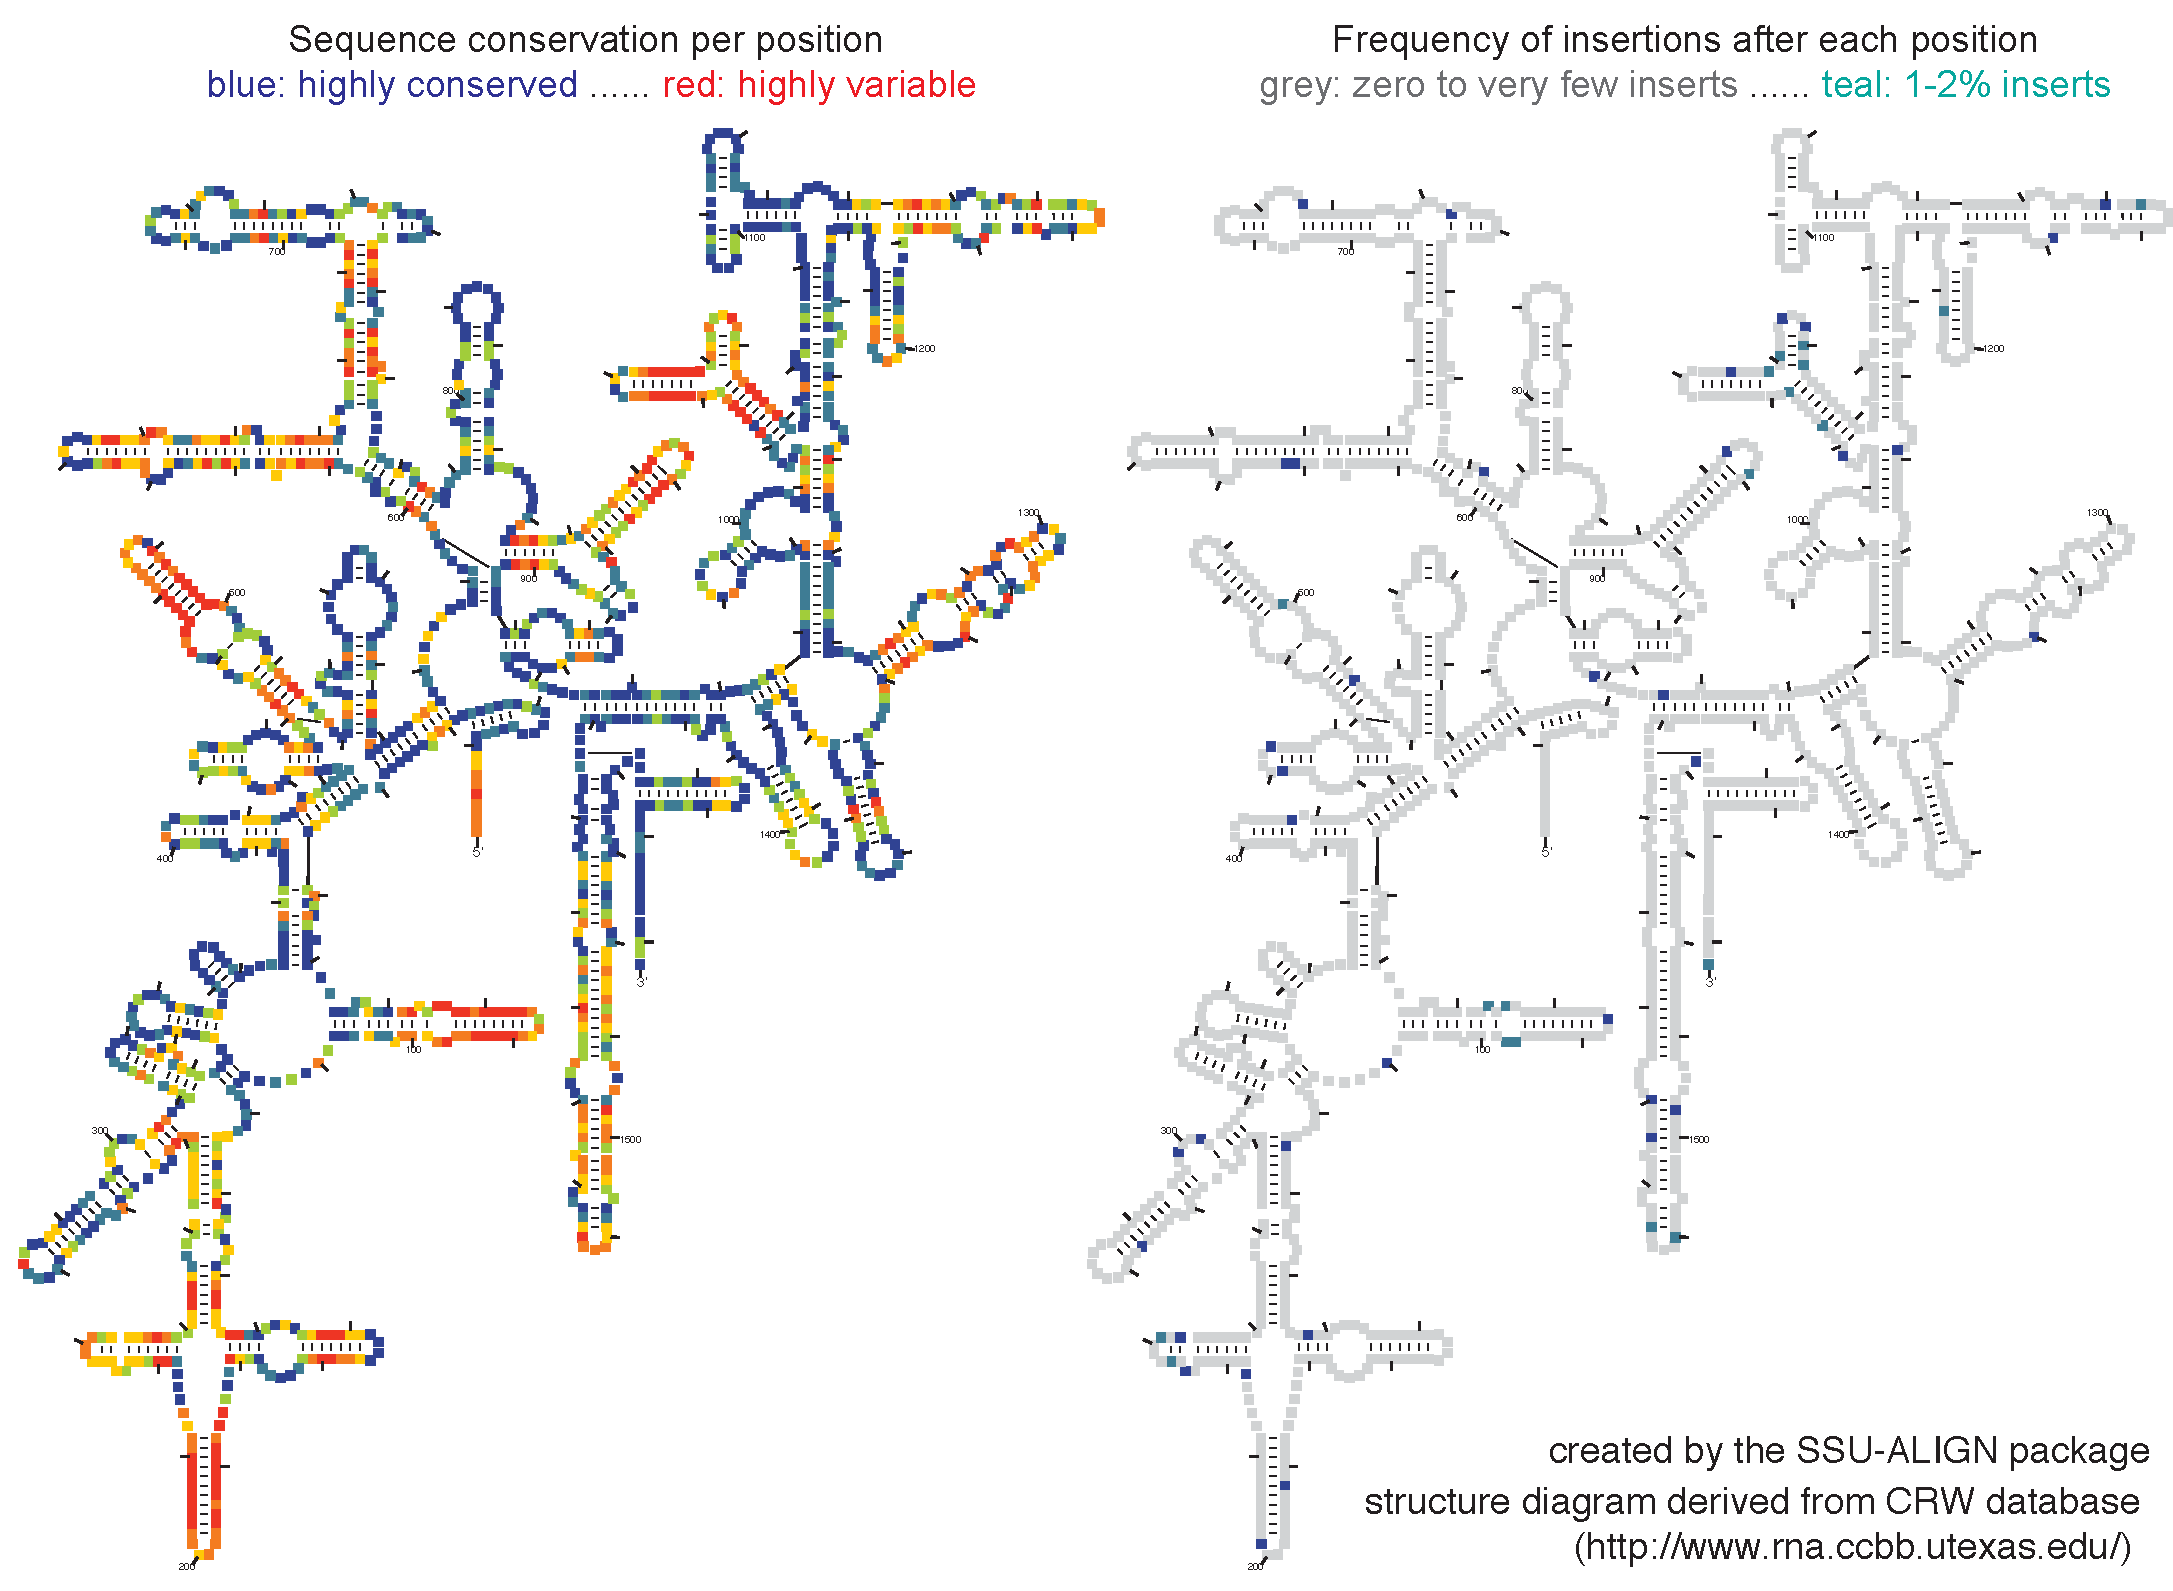
\includegraphics[width=10.5in]{figs/bacteria-info-inserts}}
\end{slide}
%%%%%%%%%%%%%%%%%%%%%%%%%%%%%%%%%%%%%%%%%%%%%%%%%%%%%%%%%%%%%%%
\begin{slide}
%\begin{center}
%\textbf{Conservation levels and insertion frequency vary in SSU rRNA}
%\end{center}
\center{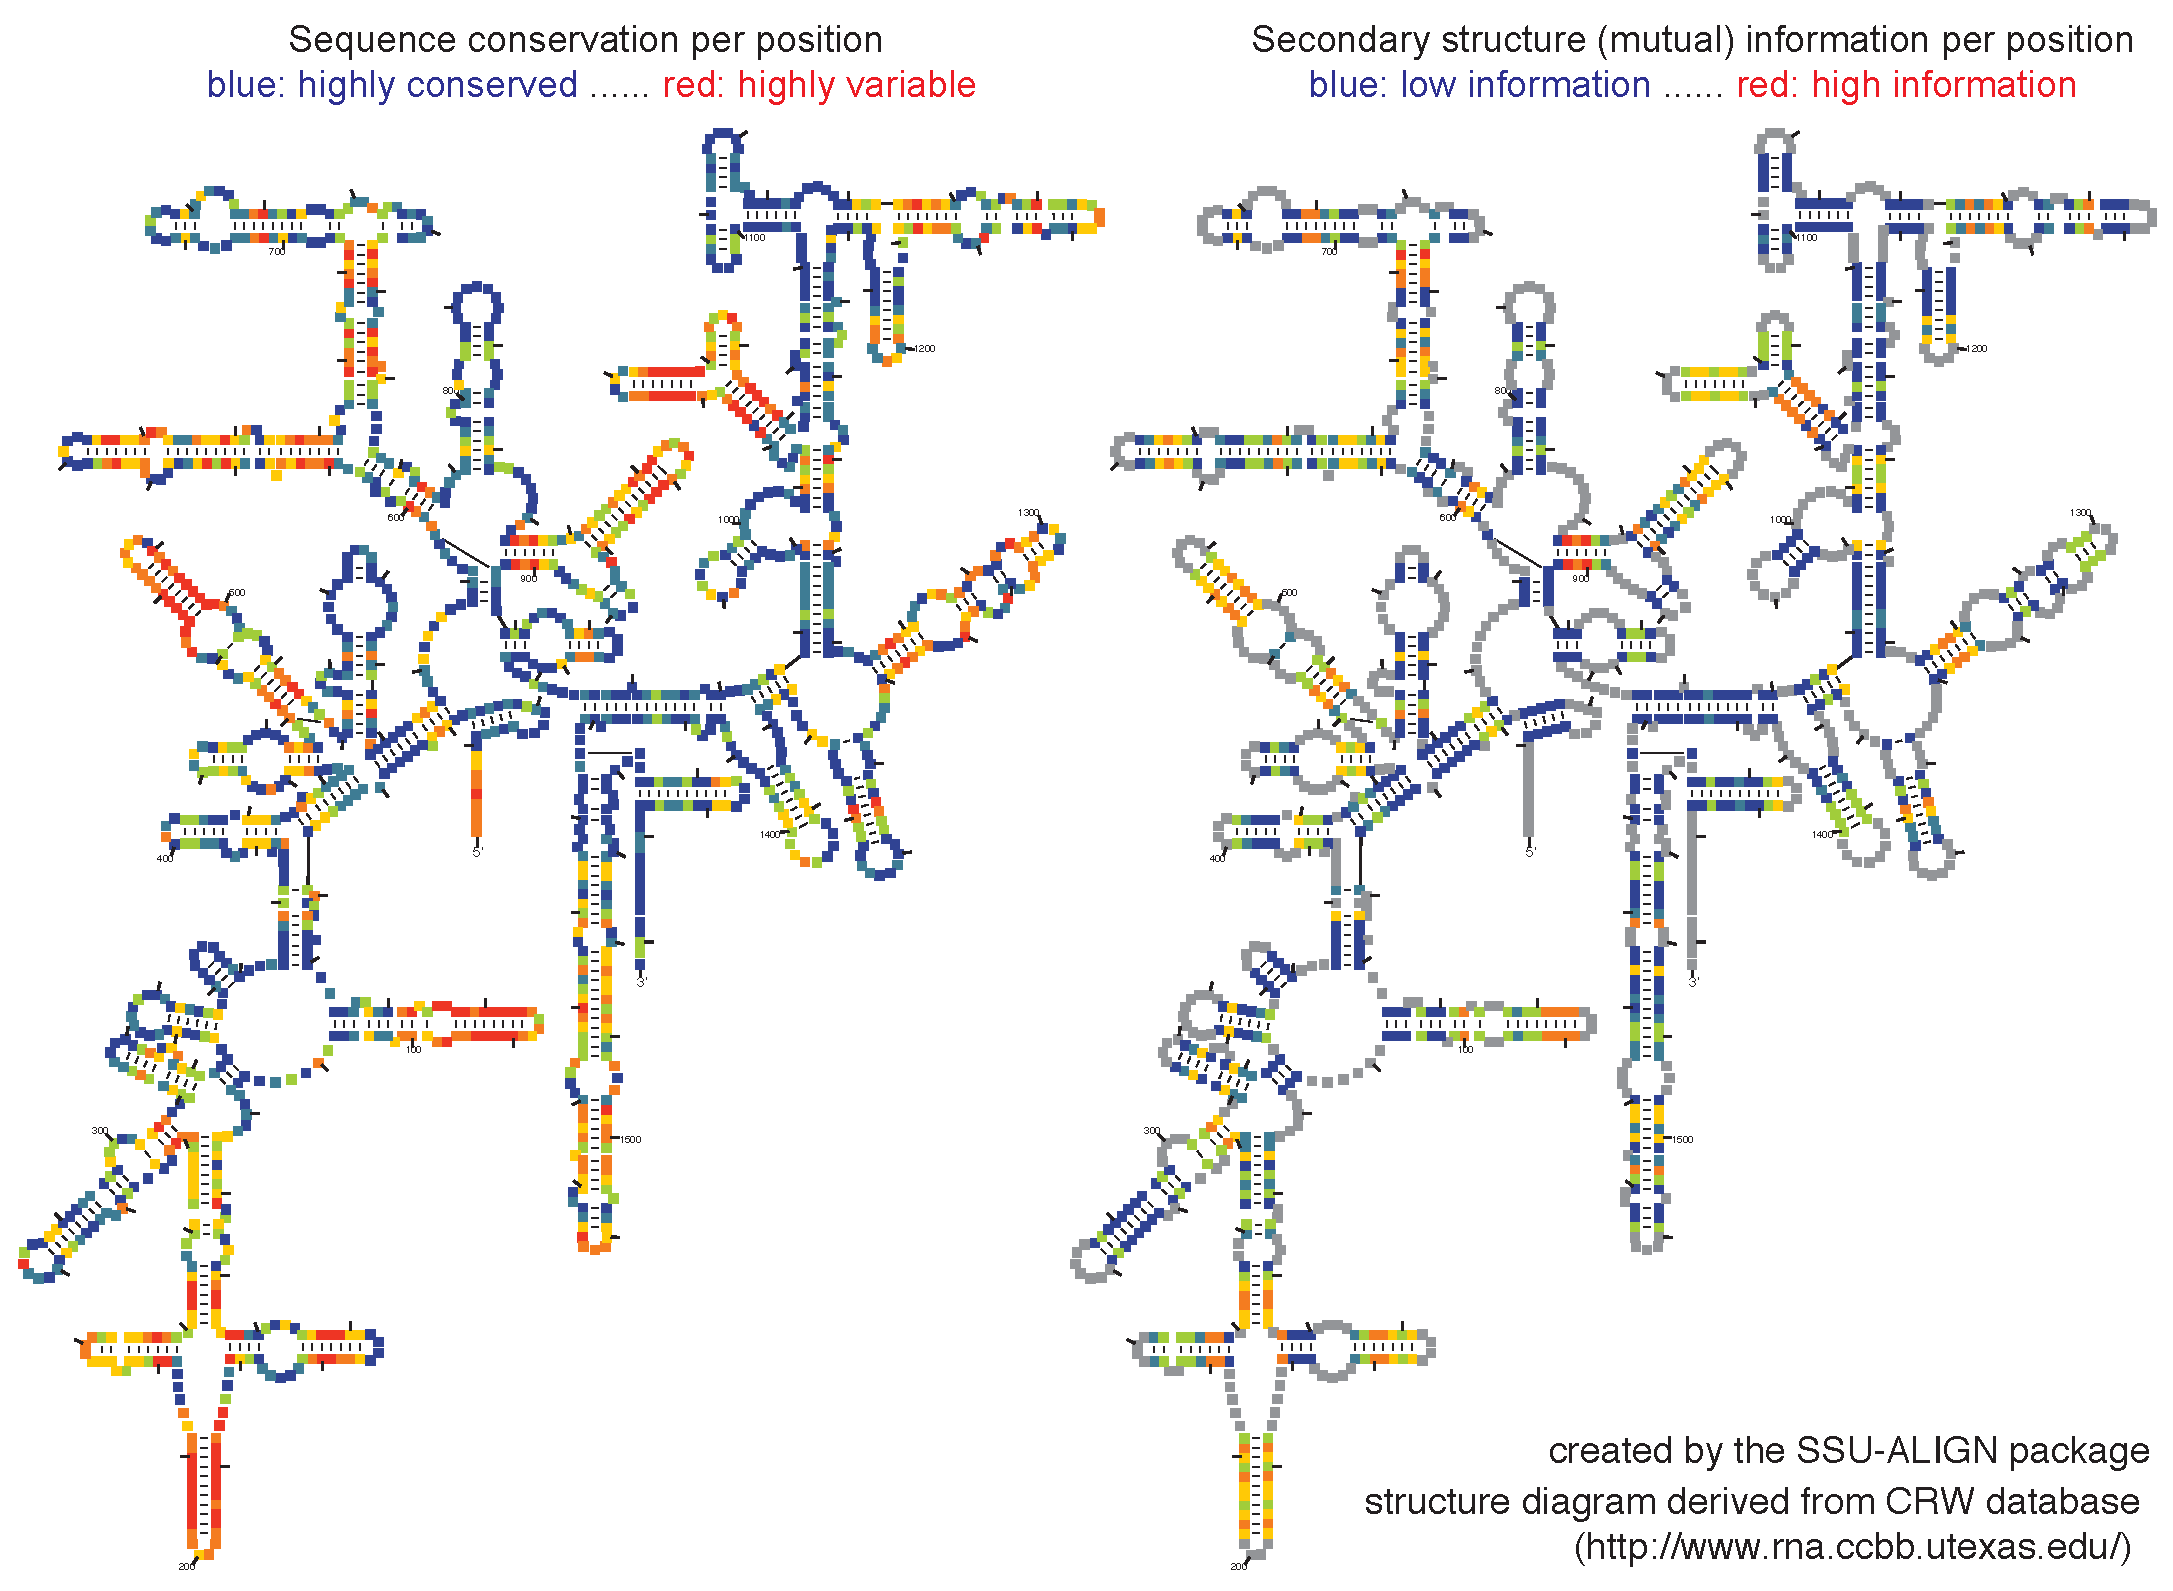
\includegraphics[width=10.5in]{figs/bacteria-info-mutinfo}}
\end{slide}
%%%%%%%%%%%%%%%%%%%%%%%%%%%%%%%%%%%%%%%%%%%%%%%%%%%%%%%%%%%%%%%
\begin{slide}
\begin{center}
%\textbf{profile HMMs and covariance models}
\textbf{Covariance models (CMs) are built \\ from structure-annotated alignments}
\end{center}
\medskip

\center{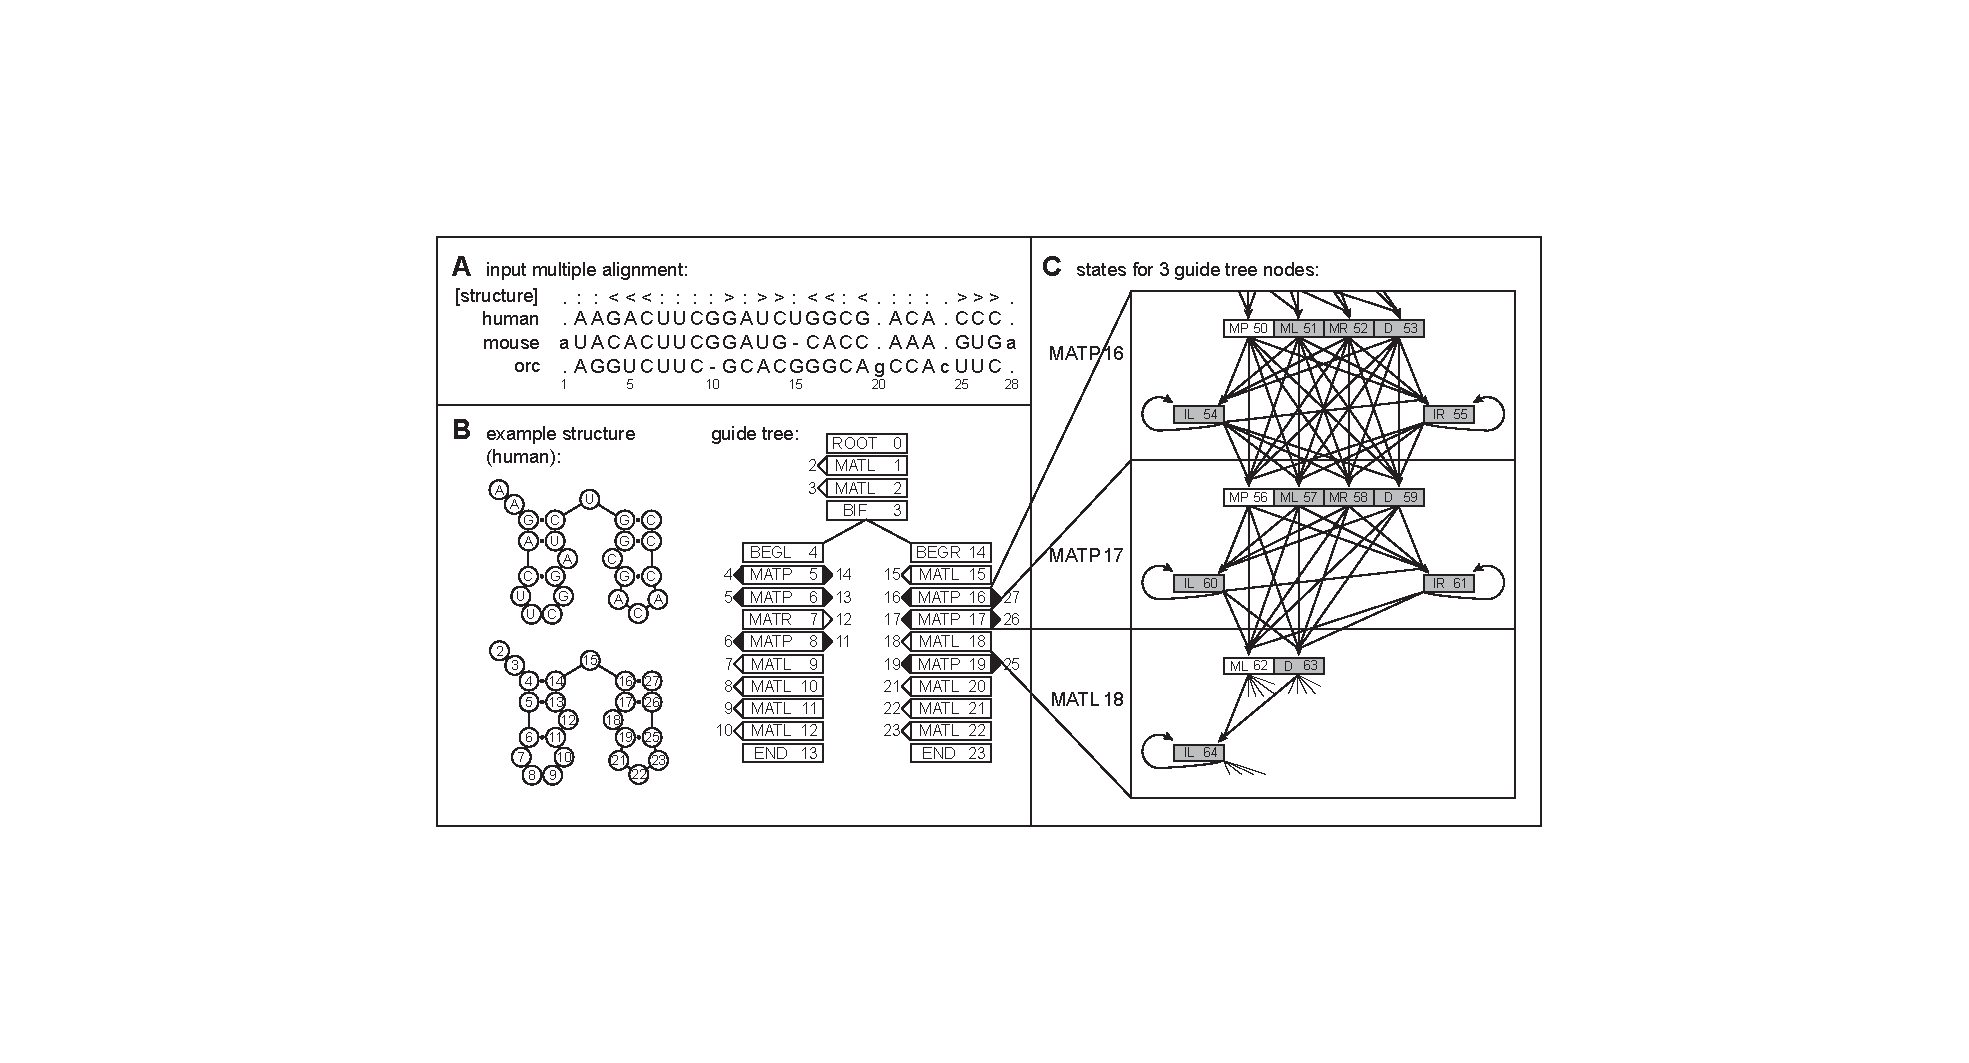
\includegraphics[width=10.5in]{figs/cmintro_bandcyk}}

%\center{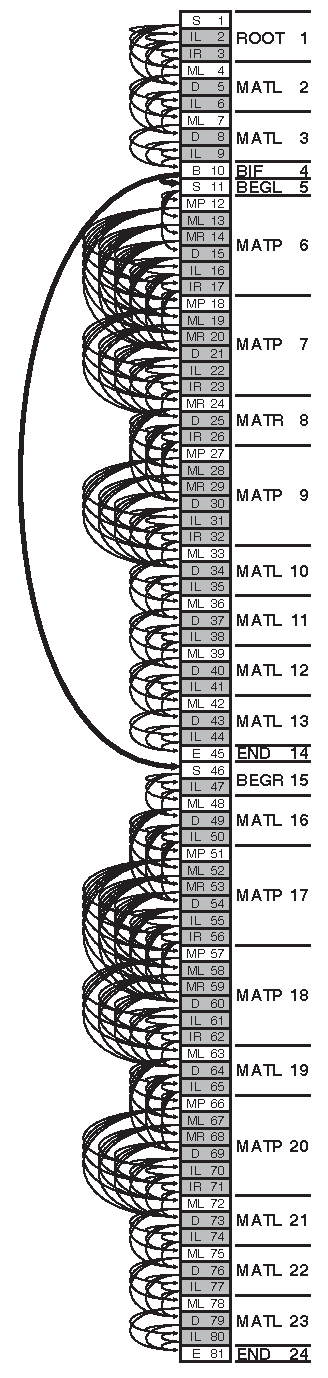
\includegraphics[width=2in,angle=270]{figs/cm-graph-small}}

%\item Extensions of profile HMMs that 

%\item Generative models that generate ``homologous'' structural RNA sequences

\vfill

\end{slide}
%%%%%%%%%%%%%%%%%%%%%%%%%%%%%%%%%%%%%%%%%%%%%%%%%%%%%%%%%%%%%%%%%%%%
\begin{slide}
\begin{center}
\textbf{Benchmark of SSU alignment}
\end{center}
\medskip

\small
\begin{itemize}
\item
How accurate are profile-based alignments?
\item
'Gold standard' testing dataset
\begin{itemize}
\item
structural alignment of 152 bacterial SSU sequences
from Robin Gutell's database
\item
this is the CRW bacterial seed alignment filtered to 92\% identity
\item
determined by 'manual' comparative analysis
\end{itemize}
\end{itemize}

\center{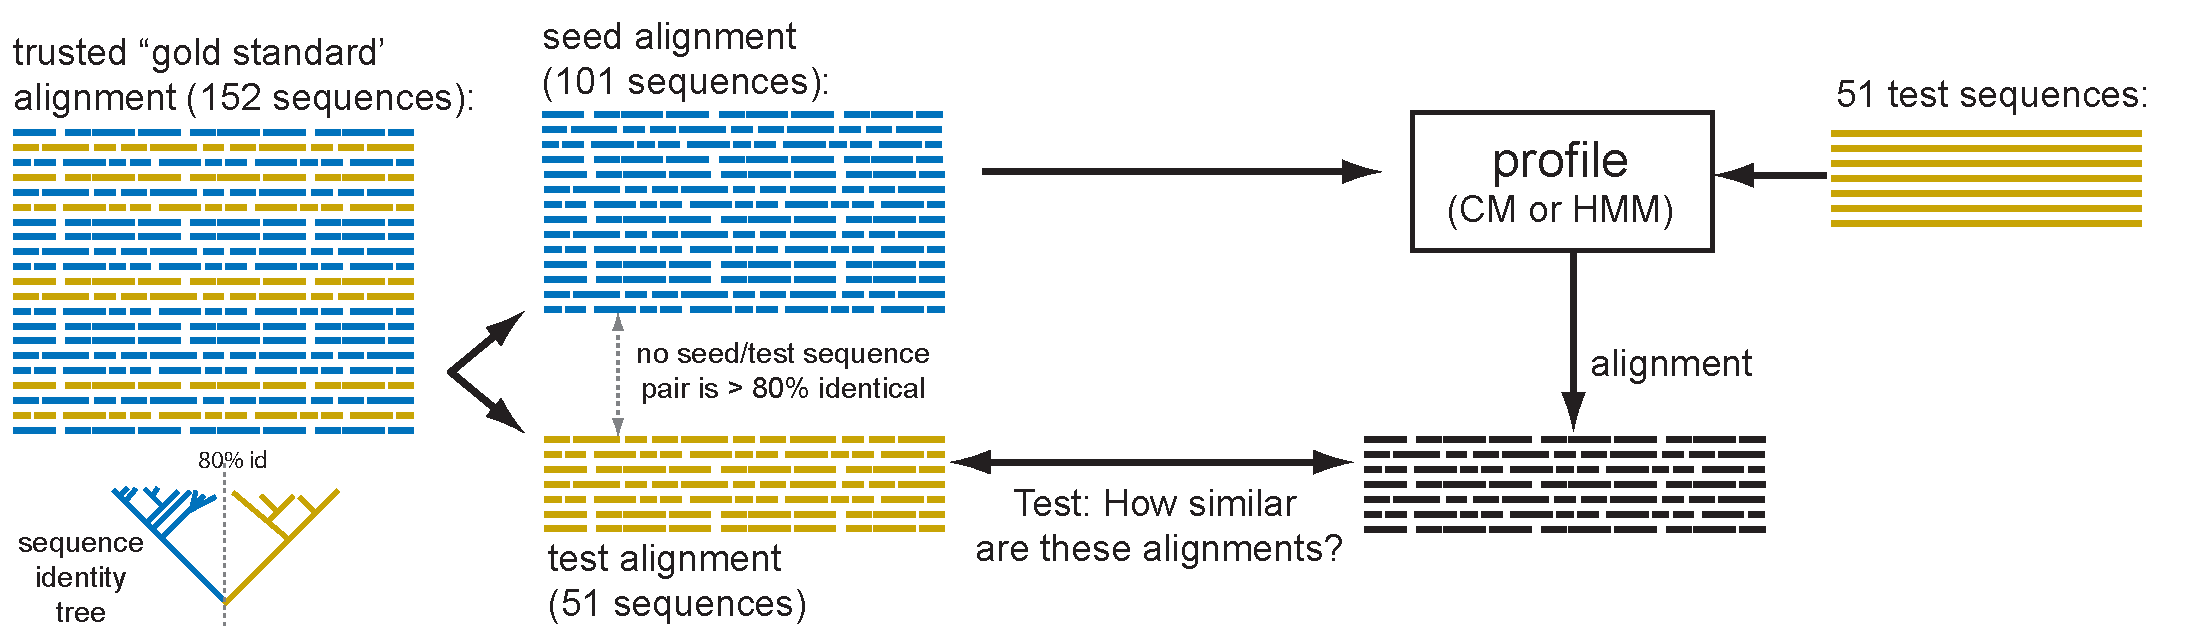
\includegraphics[width=10.5in]{figs/diana_benchmark_l2}}

\vfill
\end{slide}
%%%%%%%%%%%%%%%%%%%%%%%%%%%%%%%%%%%%%%%%%%%%%
\begin{slide}
\begin{center}
\textbf{Profiles produce accurate SSU alignments}
\end{center}
\medskip
\medskip
\begin{center}

\begin{tabular}{rcr} 
& \multicolumn{1}{c}{alignment} & \multicolumn{1}{c}{time} \\
& \multicolumn{1}{c}{accuracy} & \multicolumn{1}{c}{(sec/seq)} \\ \hline
& \multicolumn{1}{c}{} & \multicolumn{1}{c}{} \\
Muscle-3.8.31 (\emph{de novo}) & 95.4\% & 0.49 \\ 
& \multicolumn{1}{c}{} & \multicolumn{1}{c}{} \\
HMMER3 (HMMs) & 96.8\% & 0.04 \\ 
& \multicolumn{1}{c}{} & \multicolumn{1}{c}{} \\
Infernal 1.1 (CMs) & 98.1\% & 0.50 \\
& \multicolumn{1}{c}{} & \multicolumn{1}{c}{} \\
\end{tabular}
\end{center}

\vfill
\scriptsize
\flushright{Muscle: Edgar, R.C. Nucleic Acids Res 32(5), 1792-97.}
\flushright{HMMER: hmmer.janelia.org}
\flushright{Infernal: infernal.janelia.org}
\end{slide}
%%%%%%%%%%%%%%%%%%%%%%%%%%%%%%%%%%%%%%%%%%%%%%%%%%%%%%%%%%%%%%%%%%%%%%%%%
\begin{slide}
\begin{center}
\textbf{Probabilistic models allow direction calculation of useful quantities}
\end{center}

\small
\begin{itemize}
  \item Posterior decoding algorithm computes the posterior
  probability that each nucleotide is correctly aligned given the
  model
  \begin{itemize}
    \item allows HMM banding for CM alignment ($O(N^3 log(N))$ reduced
    to close to $O(N^2)$
    \item useful for identifying and removing (masking) columns that
    are not reliably aligned prior to phylogenetic inference
%    \item could be directly used during phylogenetic inference
  \end{itemize}
\end{itemize}

\center{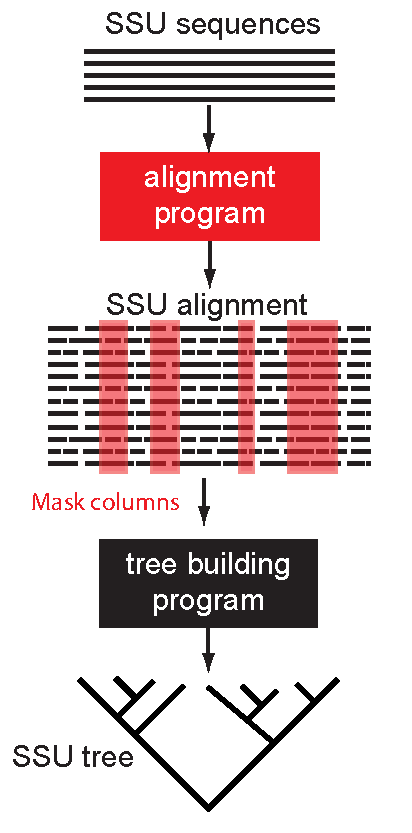
\includegraphics[height=5in]{figs/seq2tree-2013-thin-mask}}

\vfill
\end{slide}
%%%%%%%%%%%%%%%%%%%%%%%%%%%%%%%%%%%%%%%%%%%%%%%%%%%%%%%%%%%%%%%%%%%%%%%%%%
%%%%%%%%%%%%%%%%%%%%%%%%%%%%%%%%%%%%%%%%%%%%%%%%%%%%%%%%%%%%%%%%%%%%%%%%%
\begin{slide}
%\begin{center}
%
%\textbf{Phil Hugenholtz's manually created mask}
%\end{center}
%\small
\begin{center}
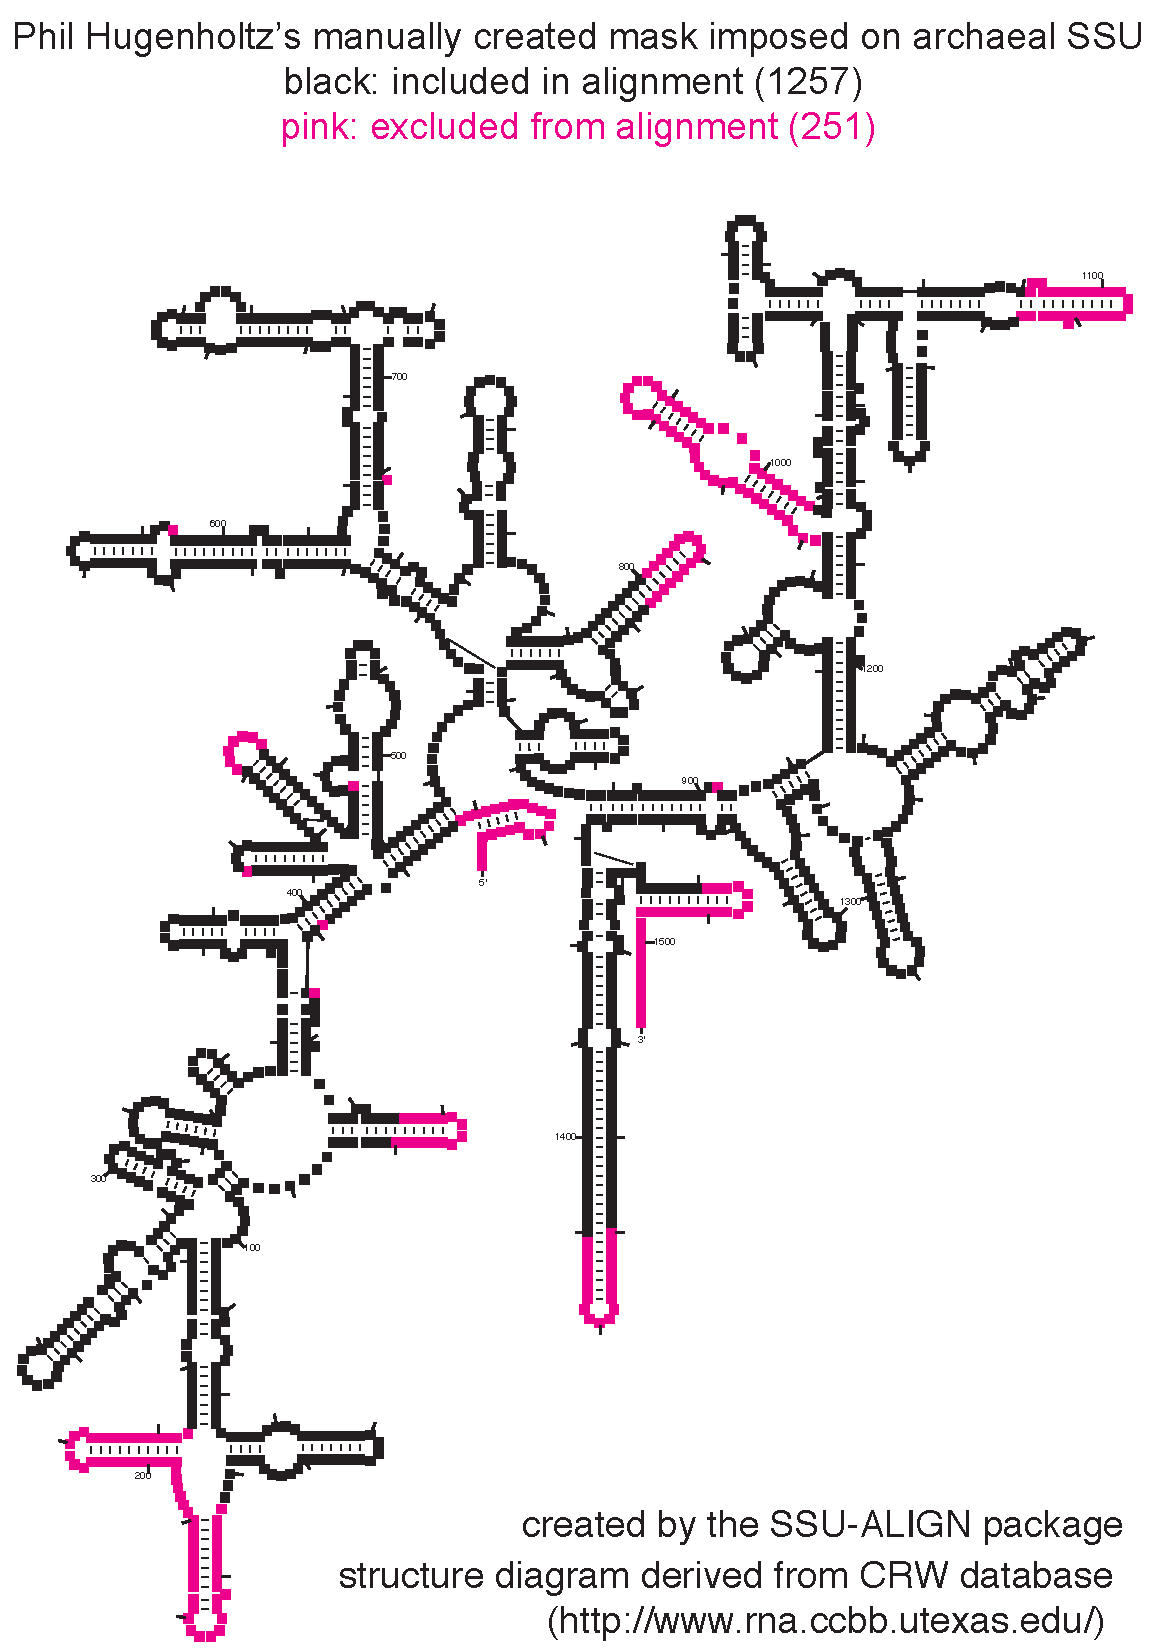
\includegraphics[height=8in]{figs/archaea-mask-ph-only}

\end{center}
\vfill
\end{slide}
%%%%%%%%%%%%%%%%%%%%%%%%%%%%%%%%%%%%%%%%%%%%%%%%%%%%%%%%%%%%%%%%%%%%%%%%%%%%%%%%%%%%%%%%%%%%%
\begin{slide}\begin{center}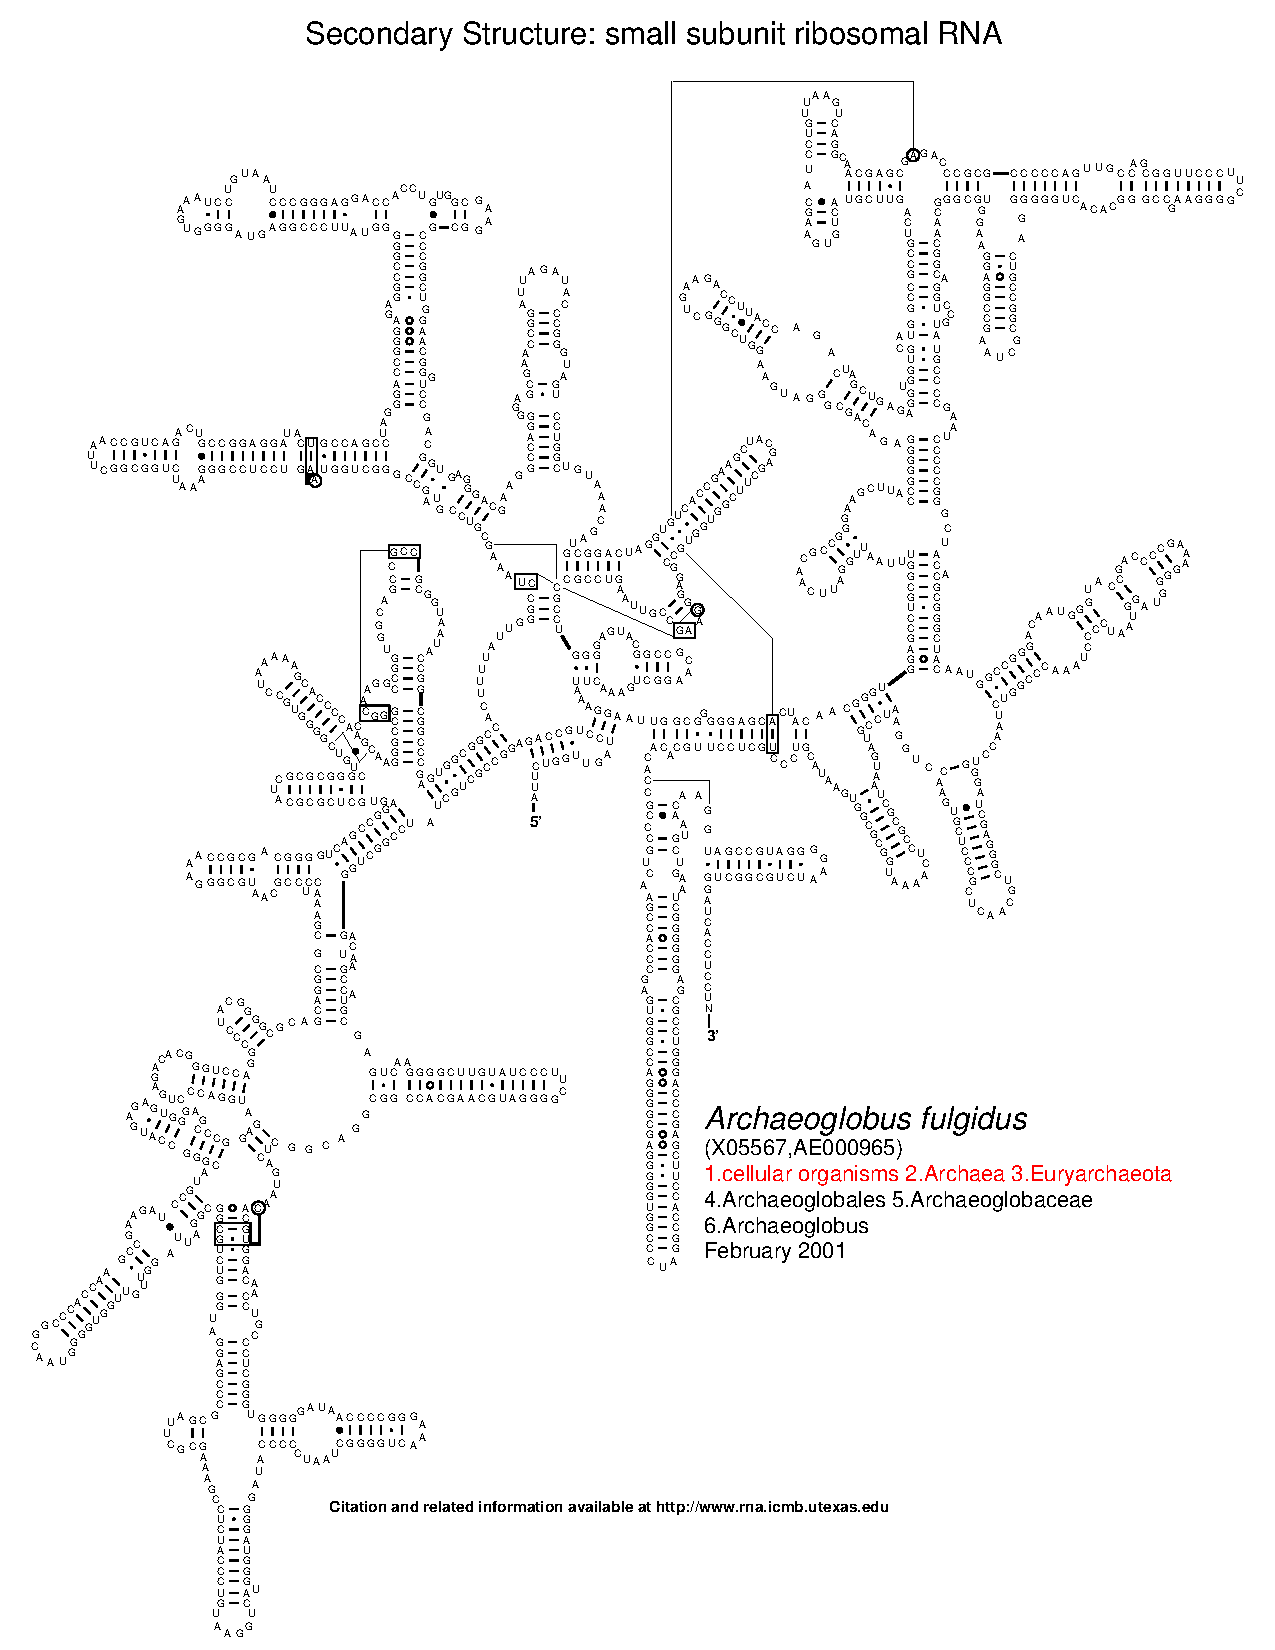
\includegraphics[height=8in]{figs/arc-1}\end{center}\vfill\end{slide}
%%%%%%%%%%%%%%%%%%%%%%%%%%%%%%%%%%%%%%%%%%%%%%%%%%%%%%%%%%%%%%%%%%%%%%%%%%%%%%%%%%%%%%%%%%%%%
\begin{slide}\begin{center}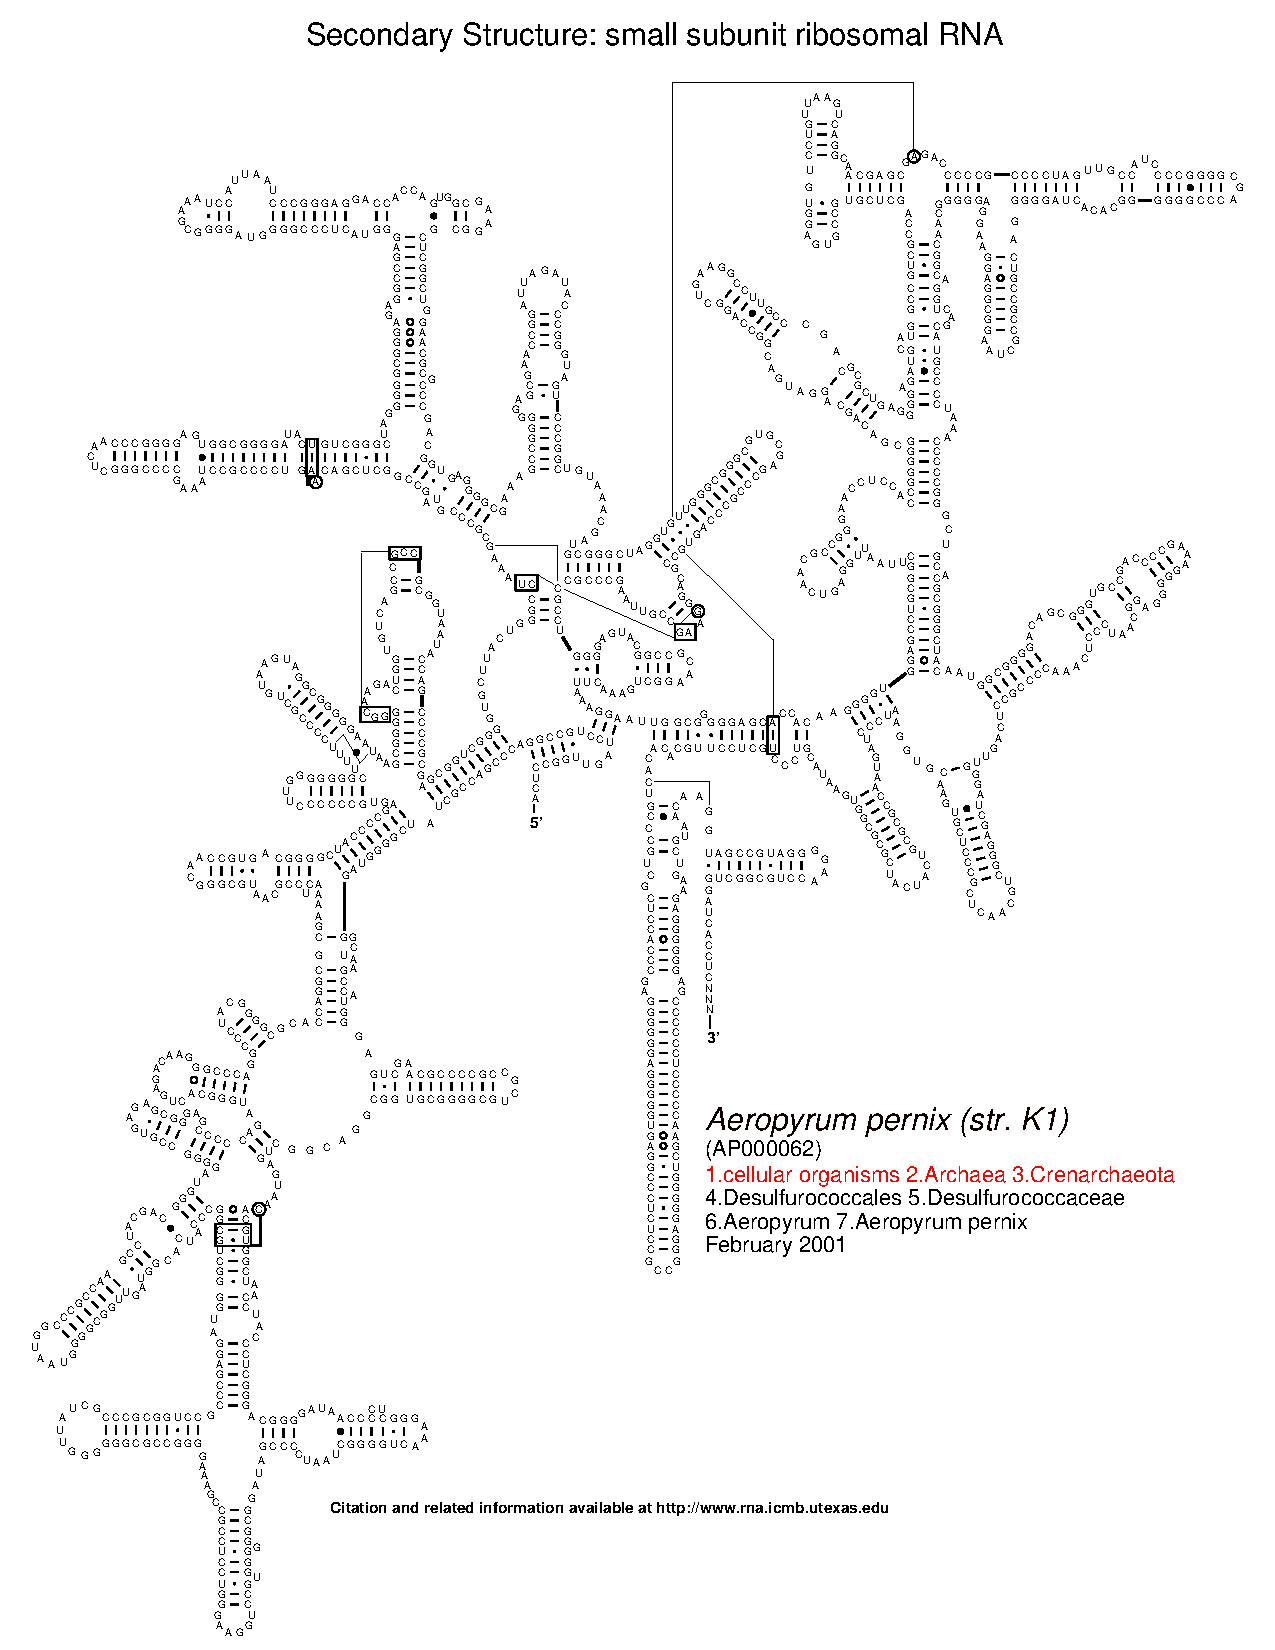
\includegraphics[height=8in]{figs/arc-2}\end{center}\vfill\end{slide}
%%%%%%%%%%%%%%%%%%%%%%%%%%%%%%%%%%%%%%%%%%%%%%%%%%%%%%%%%%%%%%%%%%%%%%%%%%%%%%%%%%%%%%%%%%%%%
\begin{slide}\begin{center}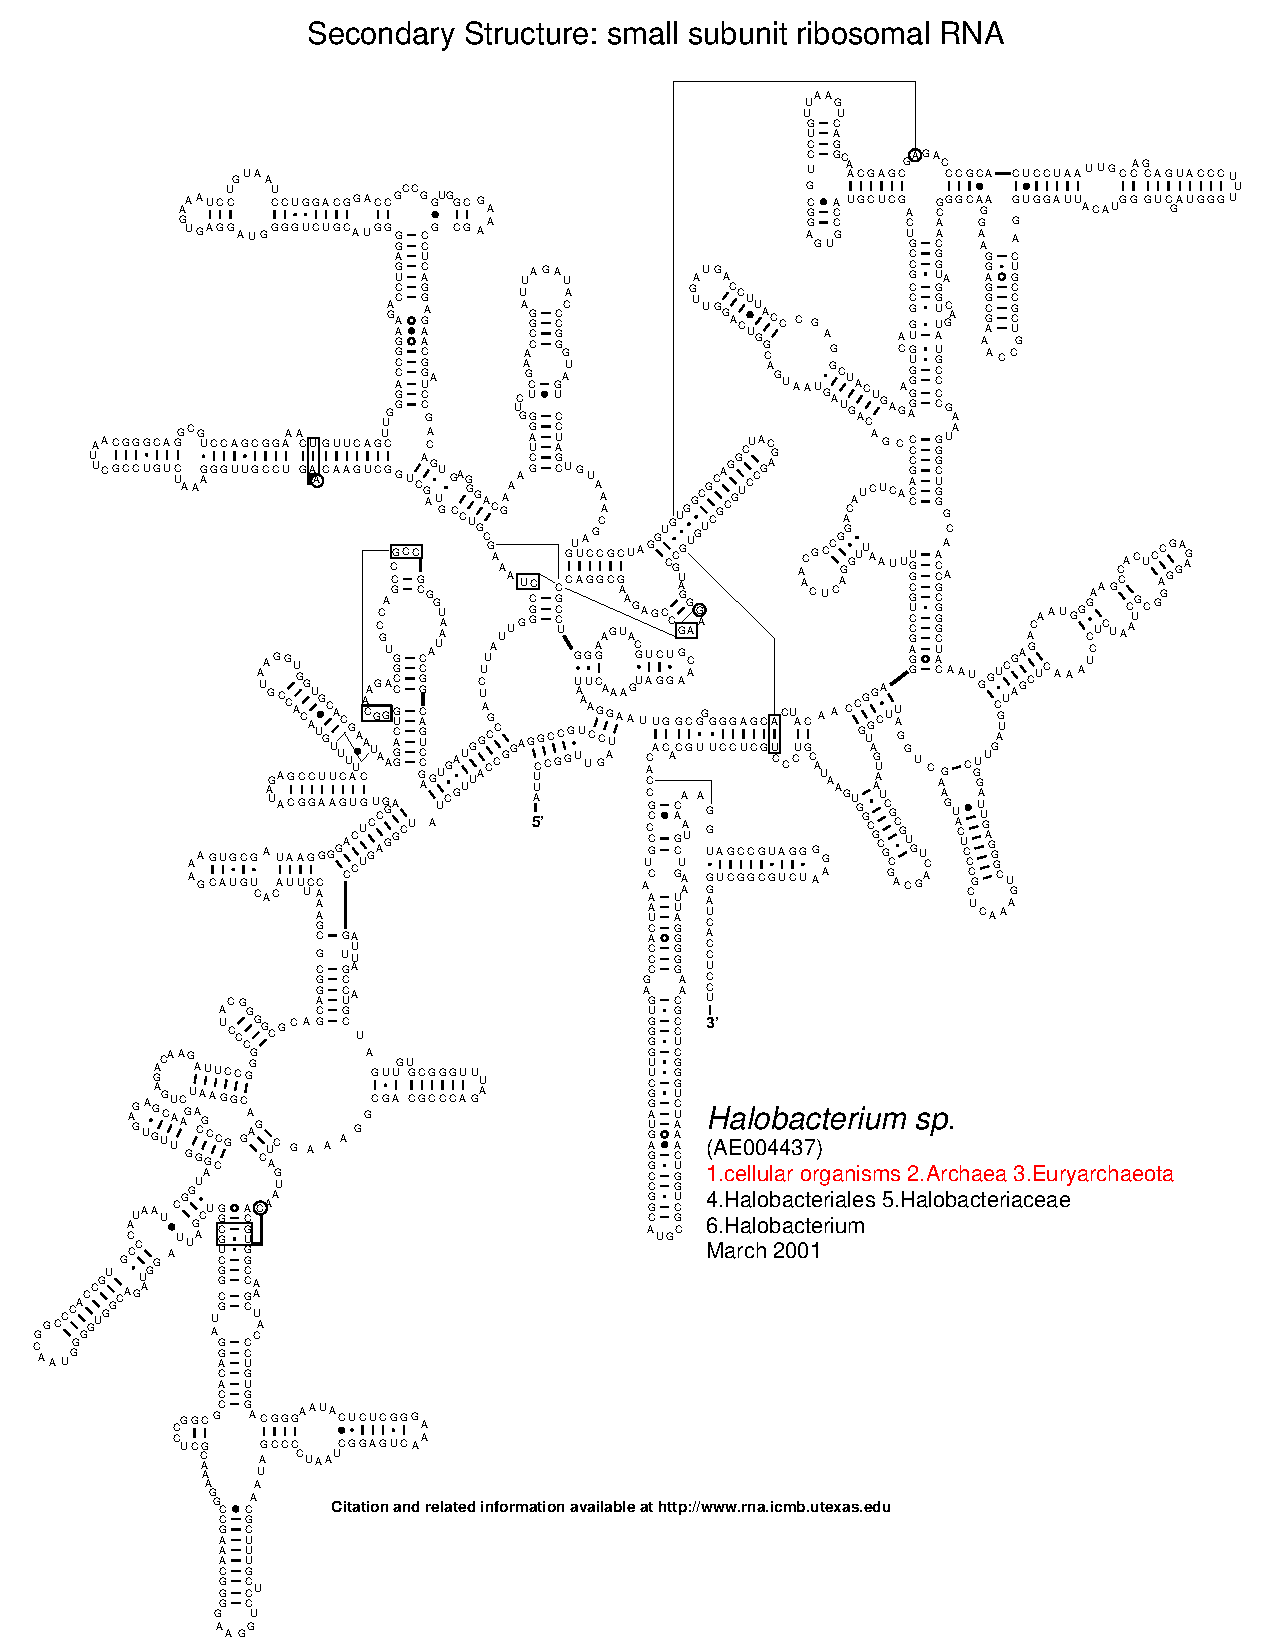
\includegraphics[height=8in]{figs/arc-3}\end{center}\vfill\end{slide}
%%%%%%%%%%%%%%%%%%%%%%%%%%%%%%%%%%%%%%%%%%%%%%%%%%%%%%%%%%%%%%%%%%%%%%%%%%%%%%%%%%%%%%%%%%%%%
%\begin{slide}\begin{center}\includegraphics[height=8in]{figs/arc-4}\end{center}\vfill\end{slide}
%%%%%%%%%%%%%%%%%%%%%%%%%%%%%%%%%%%%%%%%%%%%%%%%%%%%%%%%%%%%%%%%%%%%%%%%%%%%%%%%%%%%%%%%%%%%%
%\begin{slide}\begin{center}\includegraphics[height=8in]{figs/arc-5}\end{center}\vfill\end{slide}
%%%%%%%%%%%%%%%%%%%%%%%%%%%%%%%%%%%%%%%%%%%%%%%%%%%%%%%%%%%%%%%%%%%%%%%%%%%%%%%%%%%%%%%%%%%%%
%\begin{slide}\begin{center}\includegraphics[height=8in]{figs/arc-6}\end{center}\vfill\end{slide}
%%%%%%%%%%%%%%%%%%%%%%%%%%%%%%%%%%%%%%%%%%%%%%%%%%%%%%%%%%%%%%%%%%%%%%%%%%%%%%%%%%%%%%%%%%%%%
%\begin{slide}\begin{center}\includegraphics[height=8in]{figs/arc-7}\end{center}\vfill\end{slide}
%%%%%%%%%%%%%%%%%%%%%%%%%%%%%%%%%%%%%%%%%%%%%%%%%%%%%%%%%%%%%%%%%%%%%%%%%%%%%%%%%%%%%%%%%%%%%
%\begin{slide}\begin{center}\includegraphics[height=8in]{figs/arc-8}\end{center}\vfill\end{slide}
%%%%%%%%%%%%%%%%%%%%%%%%%%%%%%%%%%%%%%%%%%%%%%%%%%%%%%%%%%%%%%%%%%%%%%%%%%%%%%%%%%%%%%%%%%%%%
%\begin{slide}\begin{center}\includegraphics[height=8in]{figs/arc-9}\end{center}\vfill\end{slide}
%%%%%%%%%%%%%%%%%%%%%%%%%%%%%%%%%%%%%%%%%%%%%%%%%%%%%%%%%%%%%%%%%%%%%%%%%%%%%%%%%%%%%%%%%%%%%
%\begin{slide}\begin{center}\includegraphics[height=8in]{figs/arc-10}\end{center}\vfill\end{slide}
%%%%%%%%%%%%%%%%%%%%%%%%%%%%%%%%%%%%%%%%%%%%%%%%%%%%%%%%%%%%%%%%%%%%%%%%%%%%%%%%%%%%%%%%%%%%%
\begin{slide}\begin{center}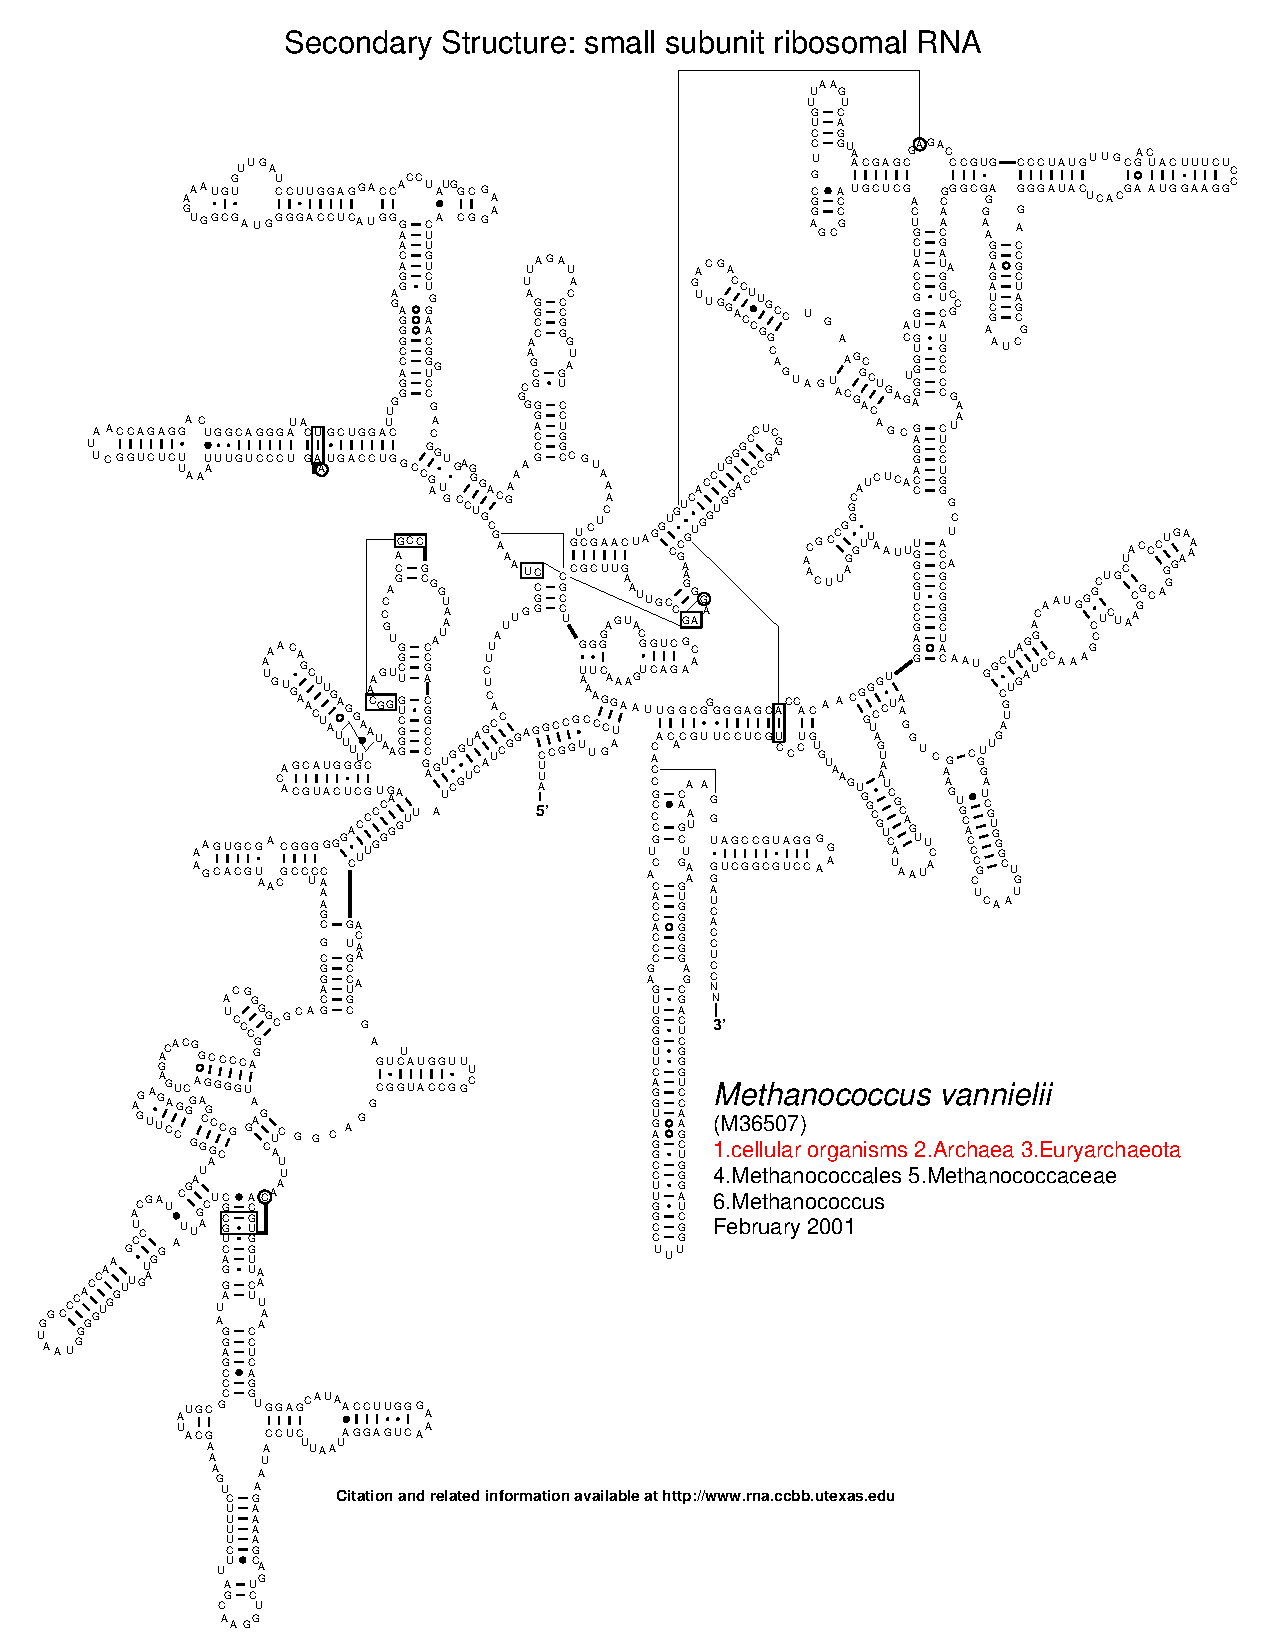
\includegraphics[height=8in]{figs/arc-11}\end{center}\vfill\end{slide}
%%%%%%%%%%%%%%%%%%%%%%%%%%%%%%%%%%%%%%%%%%%%%%%%%%%%%%%%%%%%%%%%%%%%%%%%%%%%%%%%%%%%%%%%%%%%%
\begin{slide}\begin{center}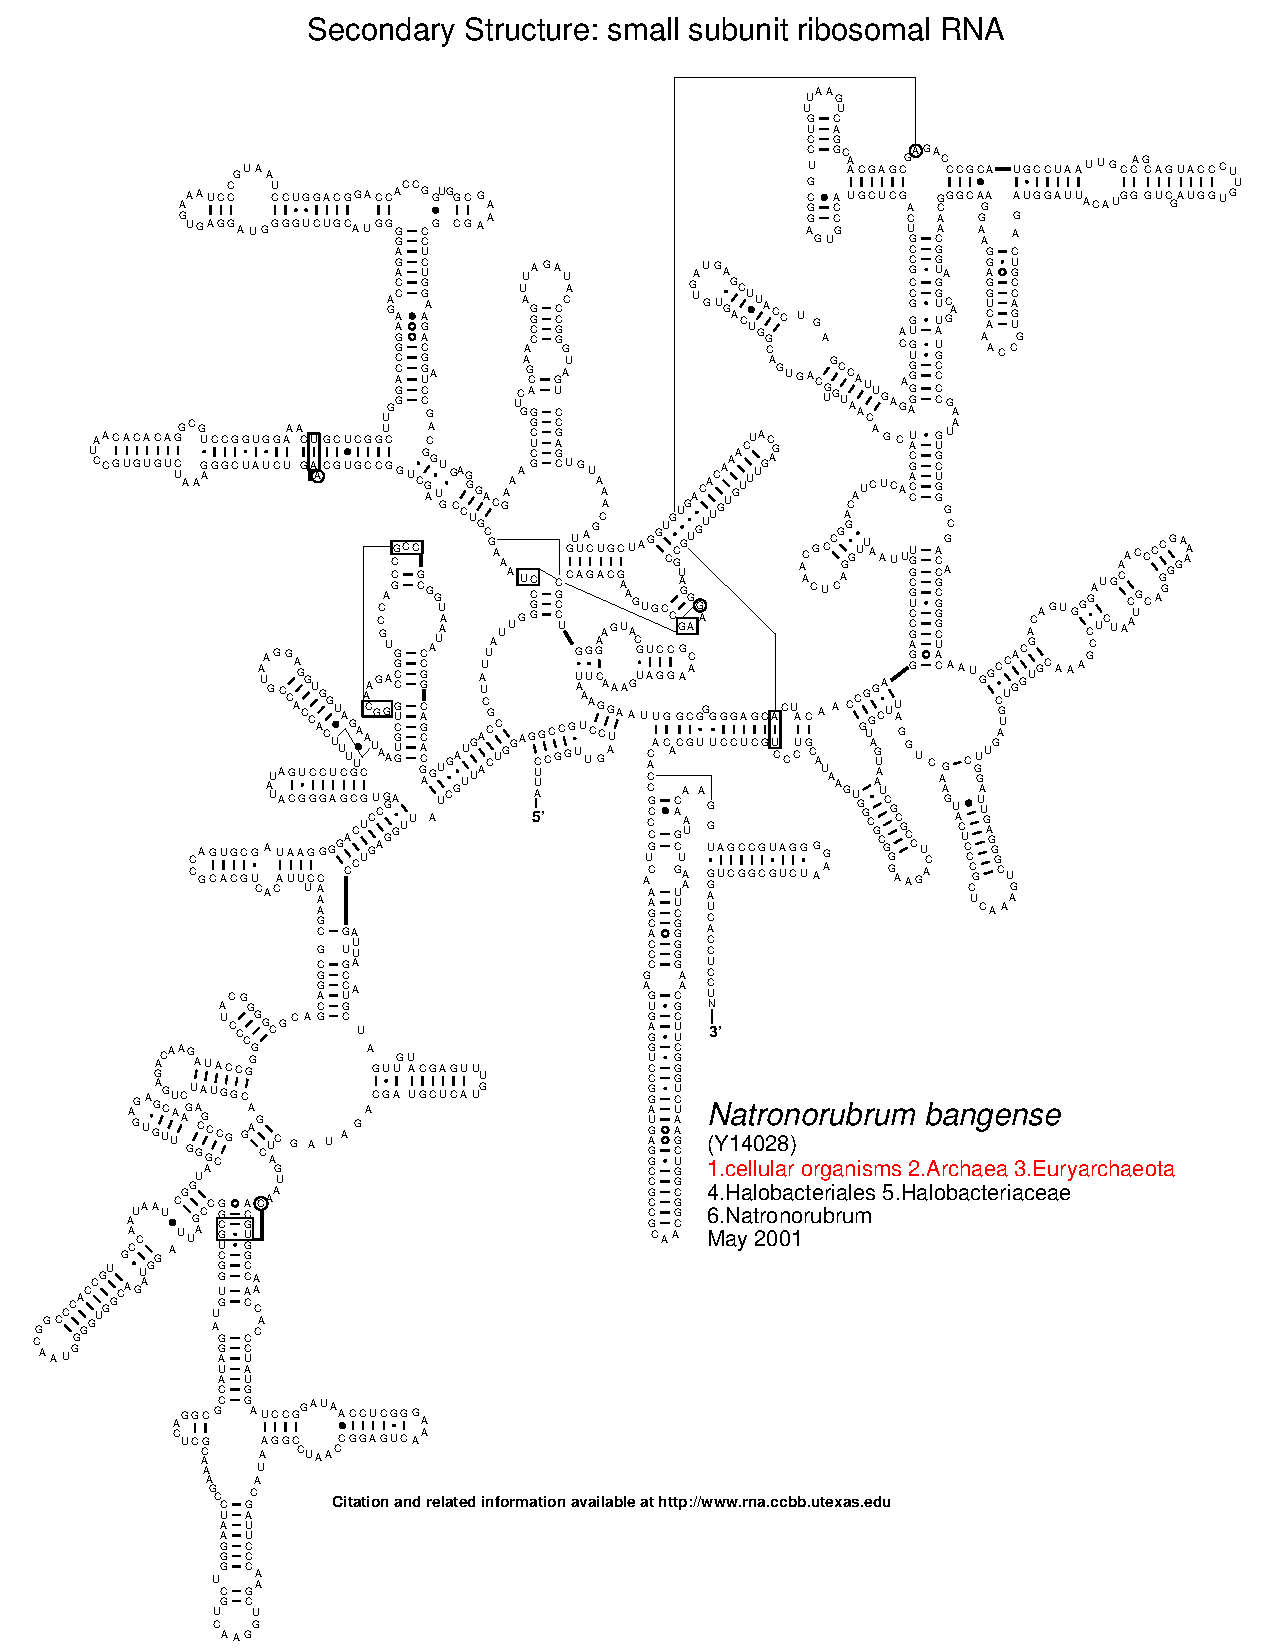
\includegraphics[height=8in]{figs/arc-12}\end{center}\vfill\end{slide}
%%%%%%%%%%%%%%%%%%%%%%%%%%%%%%%%%%%%%%%%%%%%%%%%%%%%%%%%%%%%%%%%%%%%%%%%%%%%%%%%%%%%%%%%%%%%%
\begin{slide}\begin{center}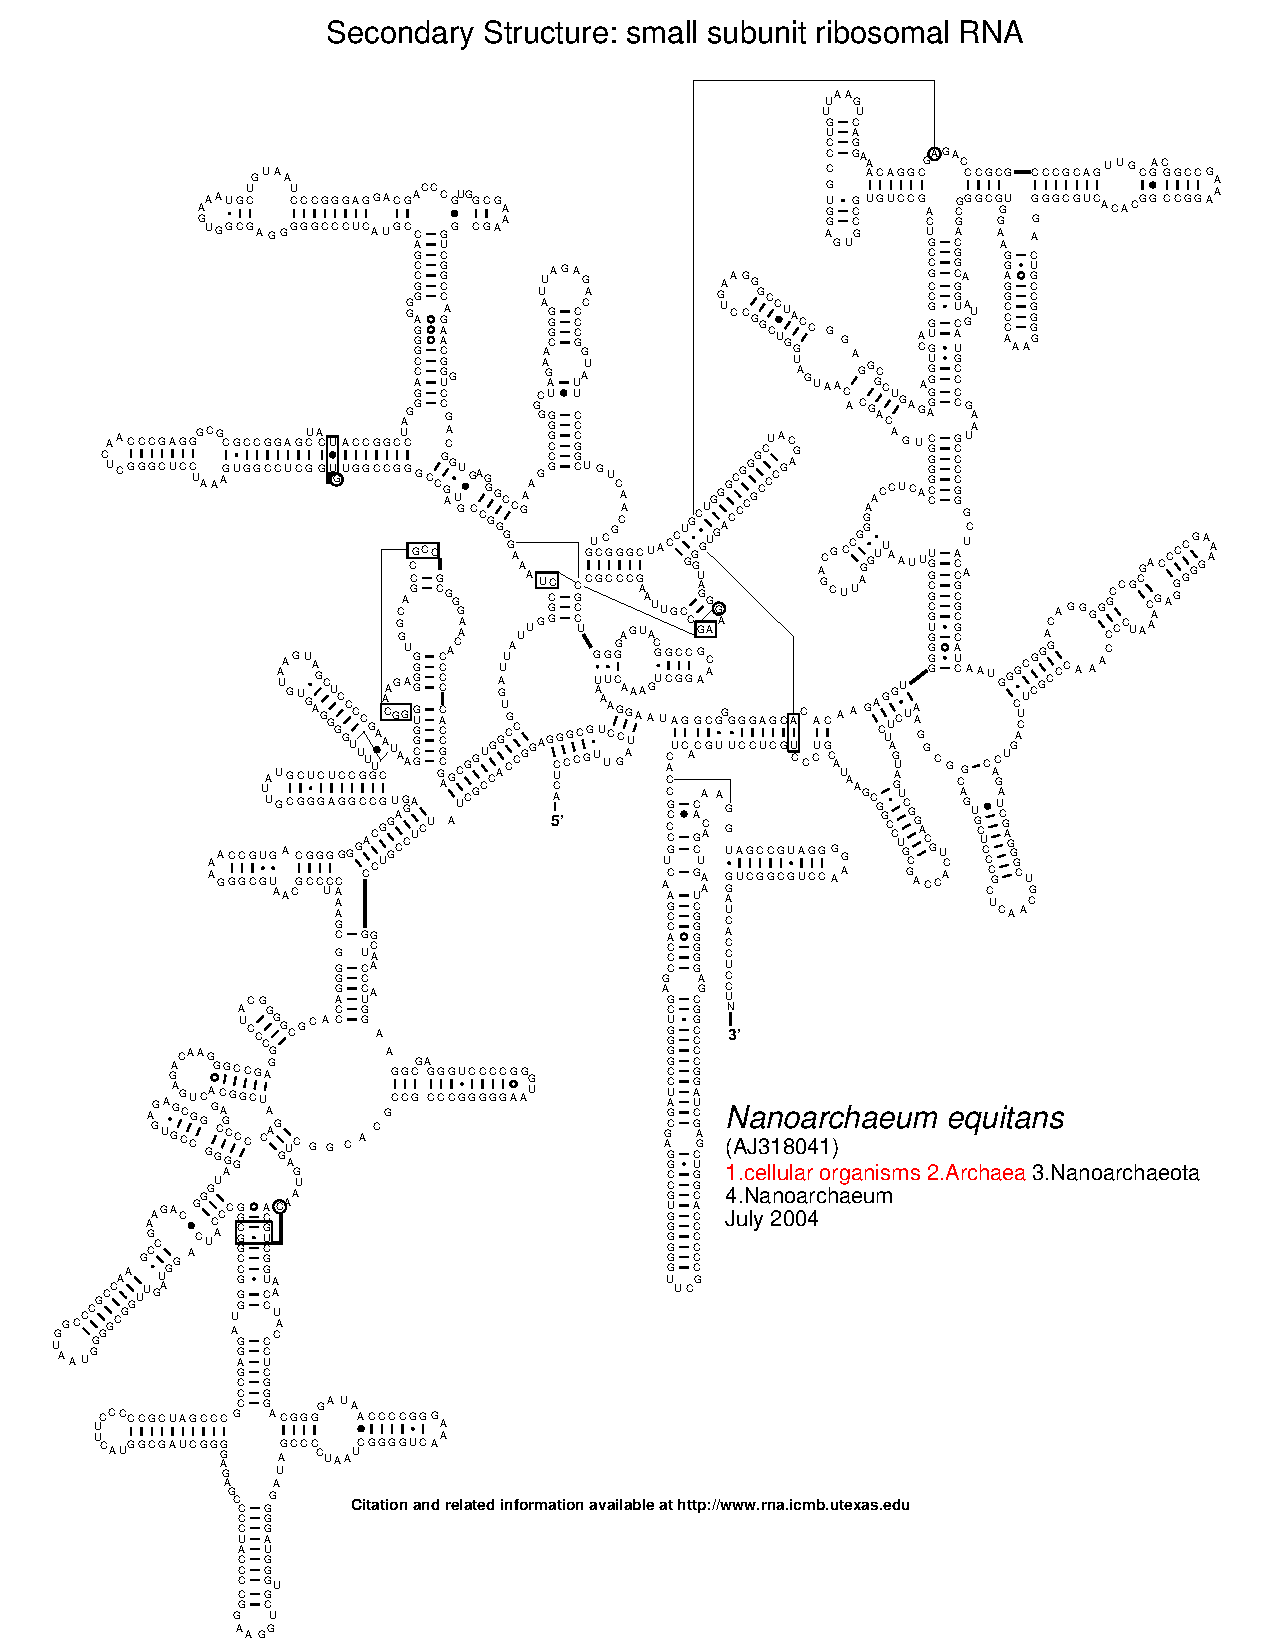
\includegraphics[height=8in]{figs/arc-13}\end{center}\vfill\end{slide}
%%%%%%%%%%%%%%%%%%%%%%%%%%%%%%%%%%%%%%%%%%%%%%%%%%%%%%%%%%%%%%%%%%%%%%%%%%%%%%%%%%%%%%%%%%%%%
\begin{slide}\begin{center}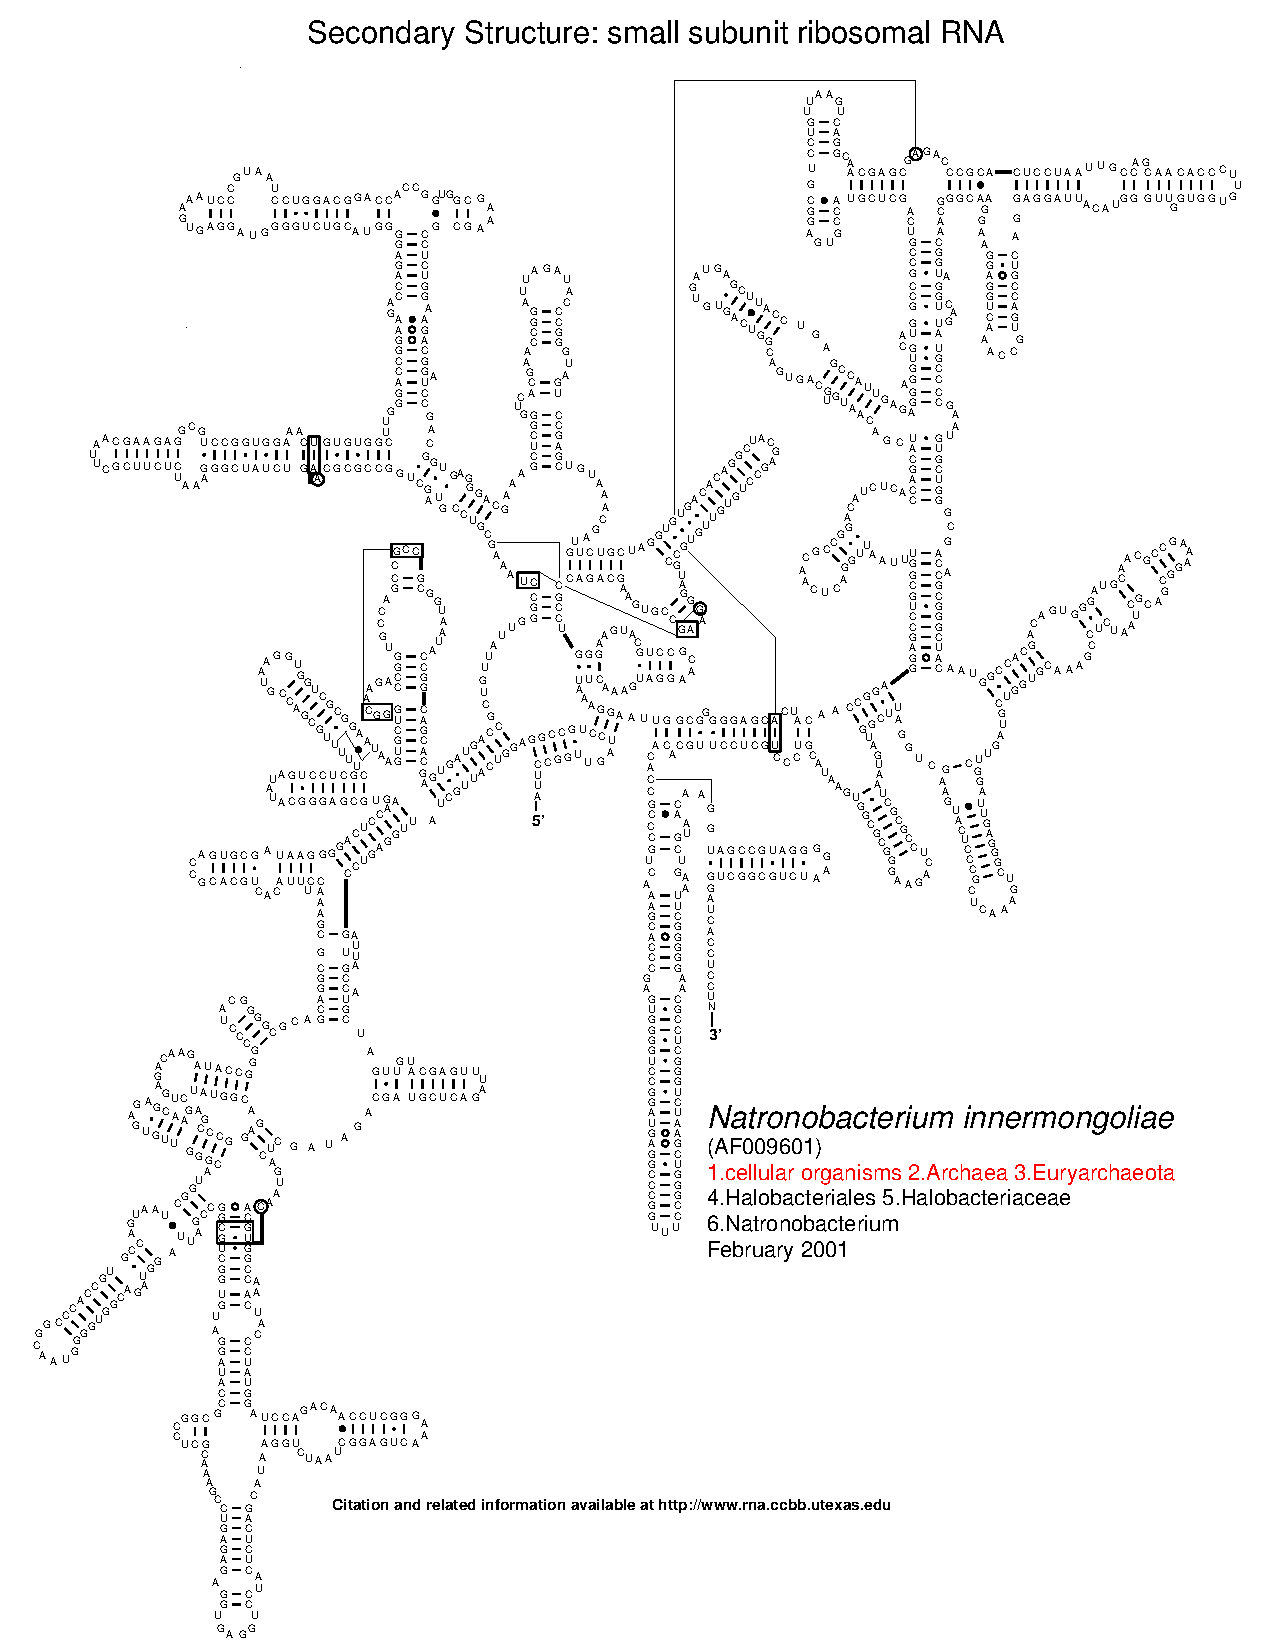
\includegraphics[height=8in]{figs/arc-14}\end{center}\vfill\end{slide}
%%%%%%%%%%%%%%%%%%%%%%%%%%%%%%%%%%%%%%%%%%%%%%%%%%%%%%%%%%%%%%%%%%%%%%%%%%%%%%%%%%%%%%%%%%%%%
\begin{slide}\begin{center}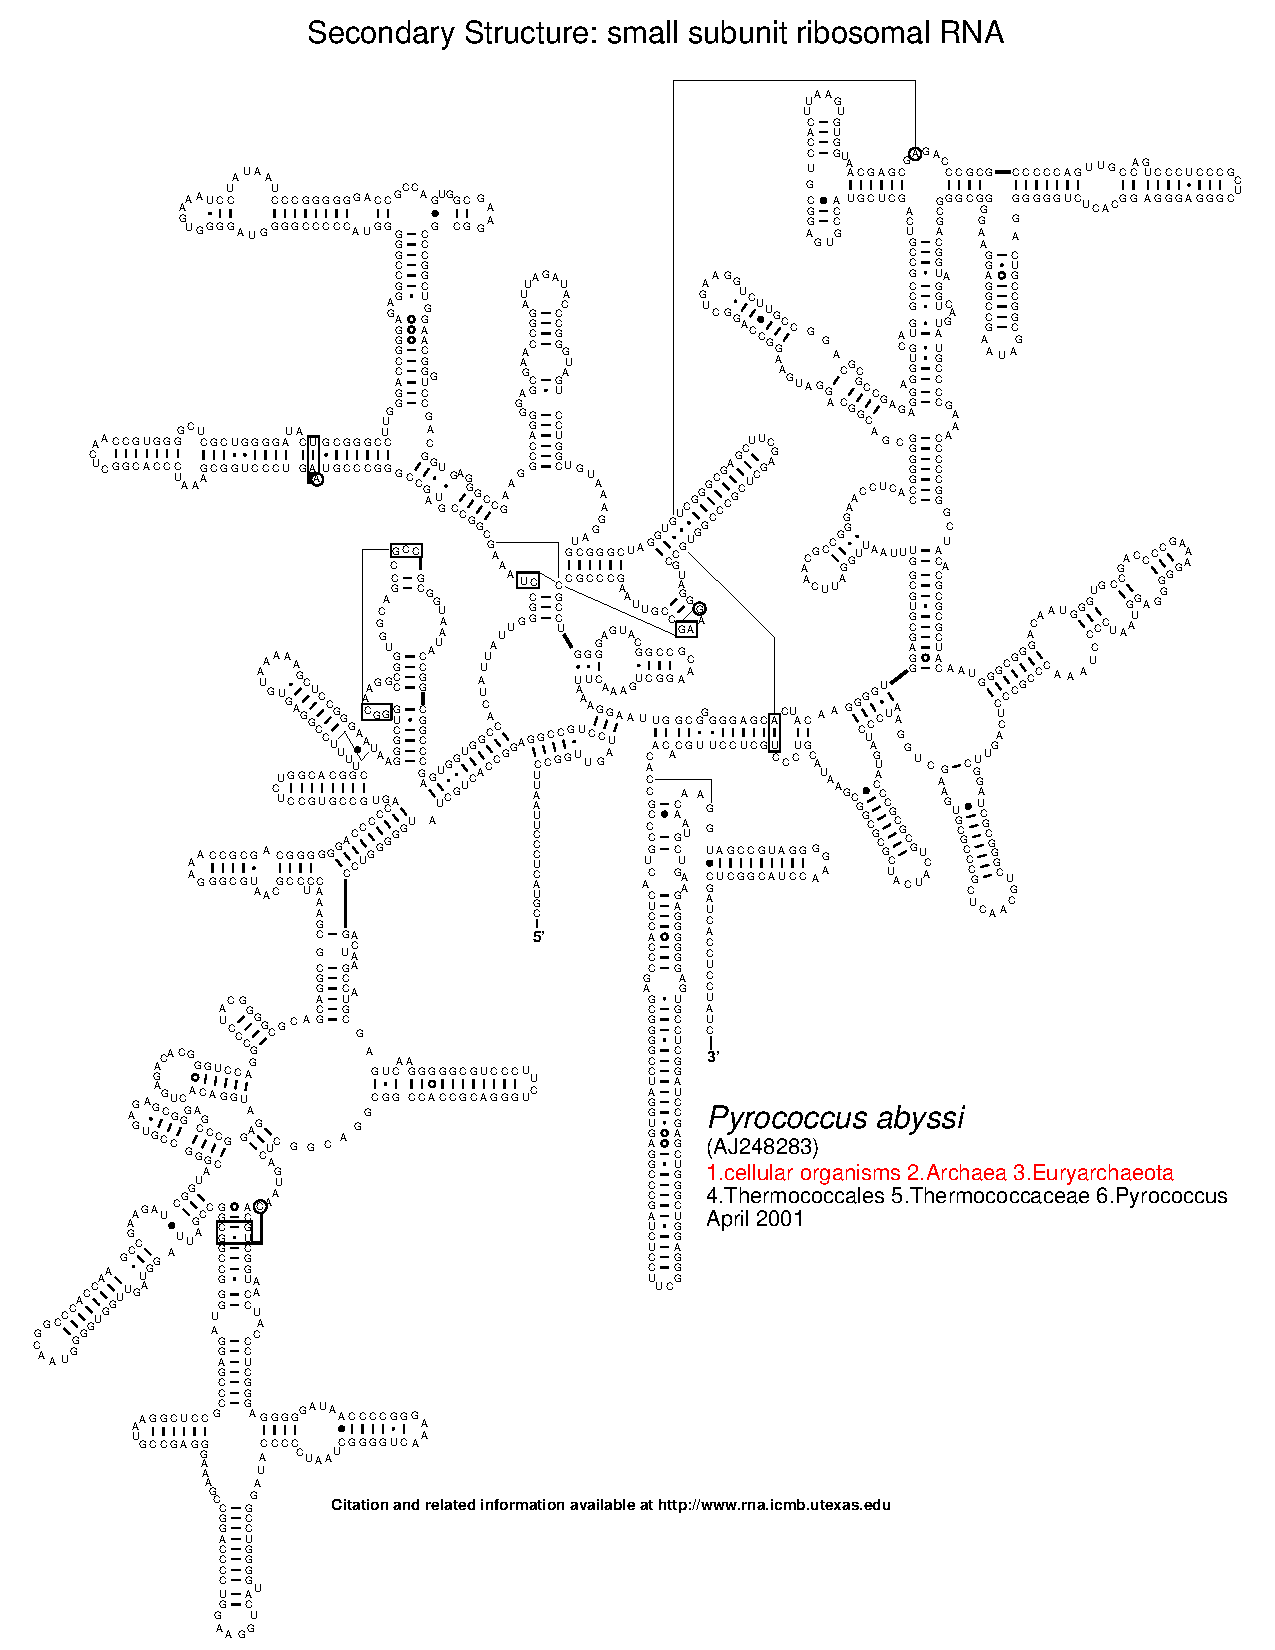
\includegraphics[height=8in]{figs/arc-15}\end{center}\vfill\end{slide}
%%%%%%%%%%%%%%%%%%%%%%%%%%%%%%%%%%%%%%%%%%%%%%%%%%%%%%%%%%%%%%%%%%%%%%%%%%%%%%%%%%%%%%%%%%%%%
\begin{slide}\begin{center}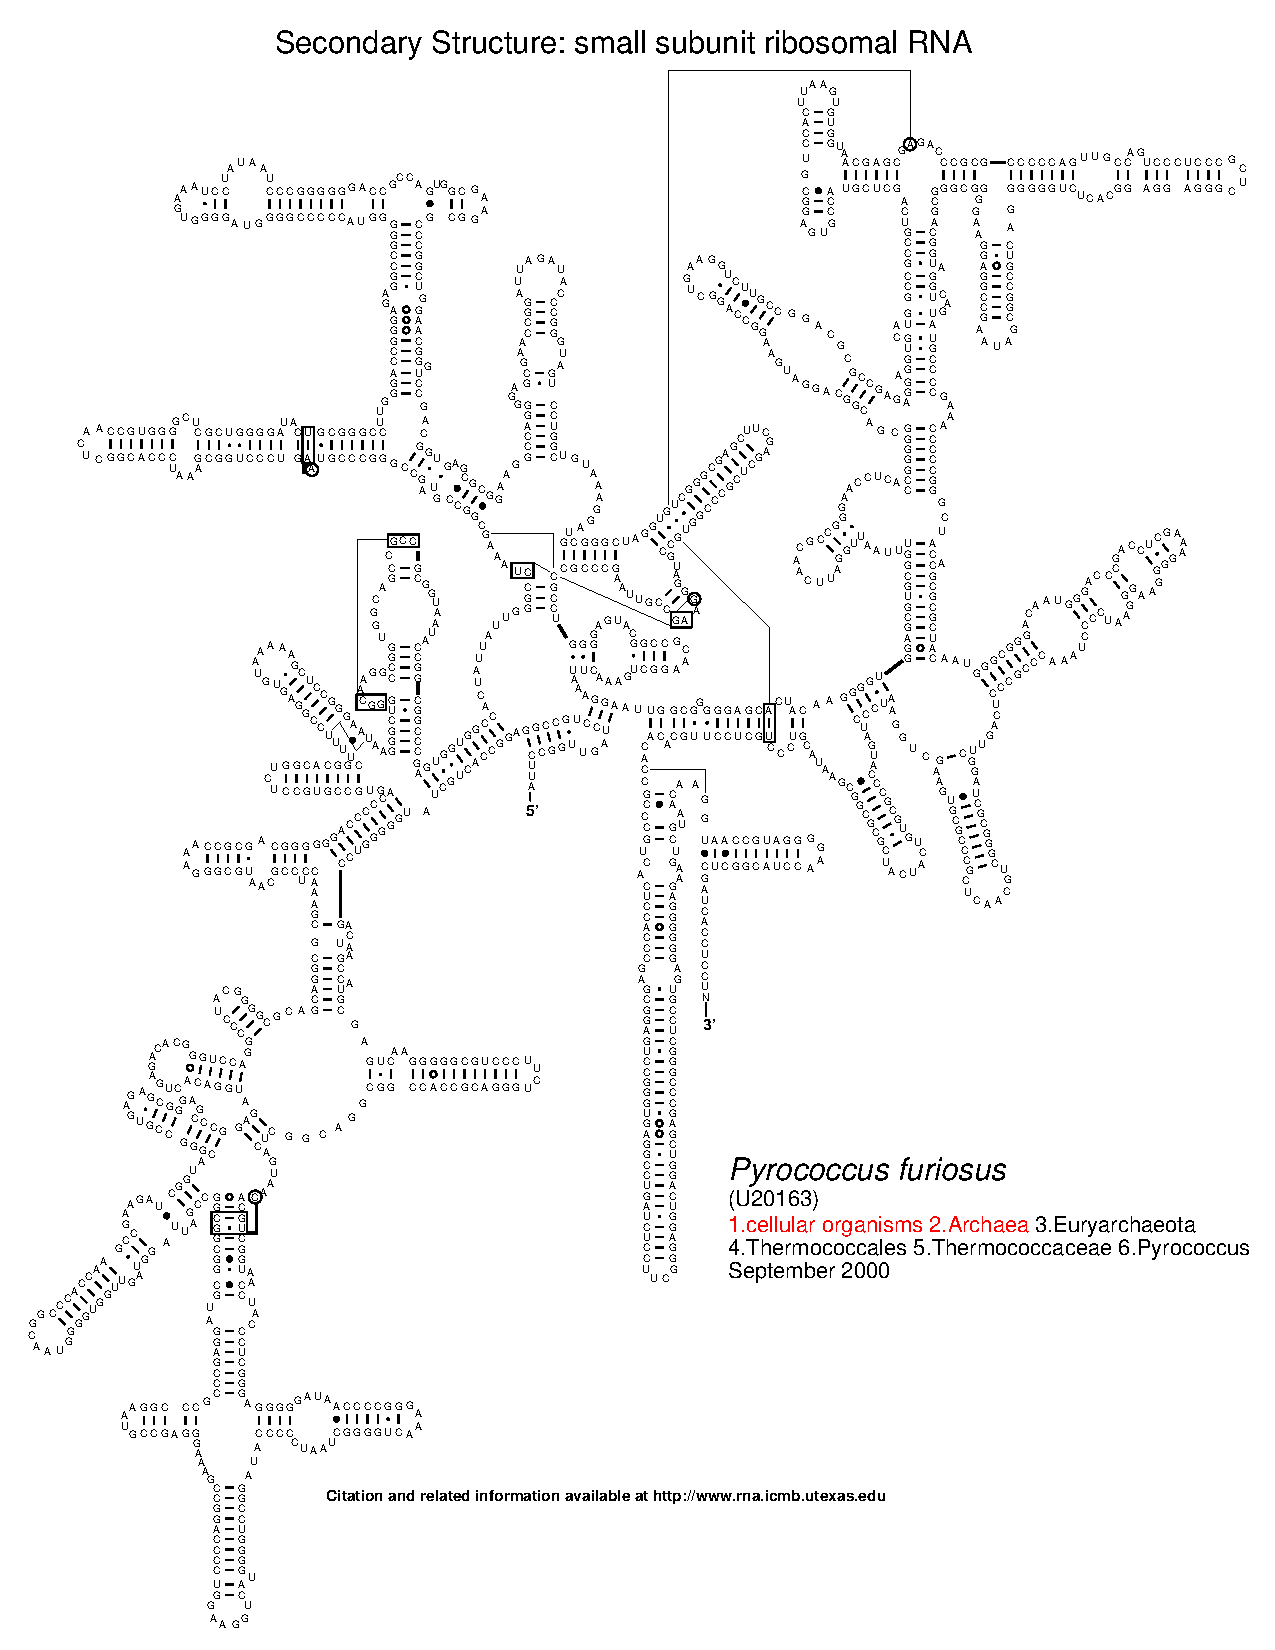
\includegraphics[height=8in]{figs/arc-16}\end{center}\vfill\end{slide}
%%%%%%%%%%%%%%%%%%%%%%%%%%%%%%%%%%%%%%%%%%%%%%%%%%%%%%%%%%%%%%%%%%%%%%%%%%%%%%%%%%%%%%%%%%%%%
\begin{slide}\begin{center}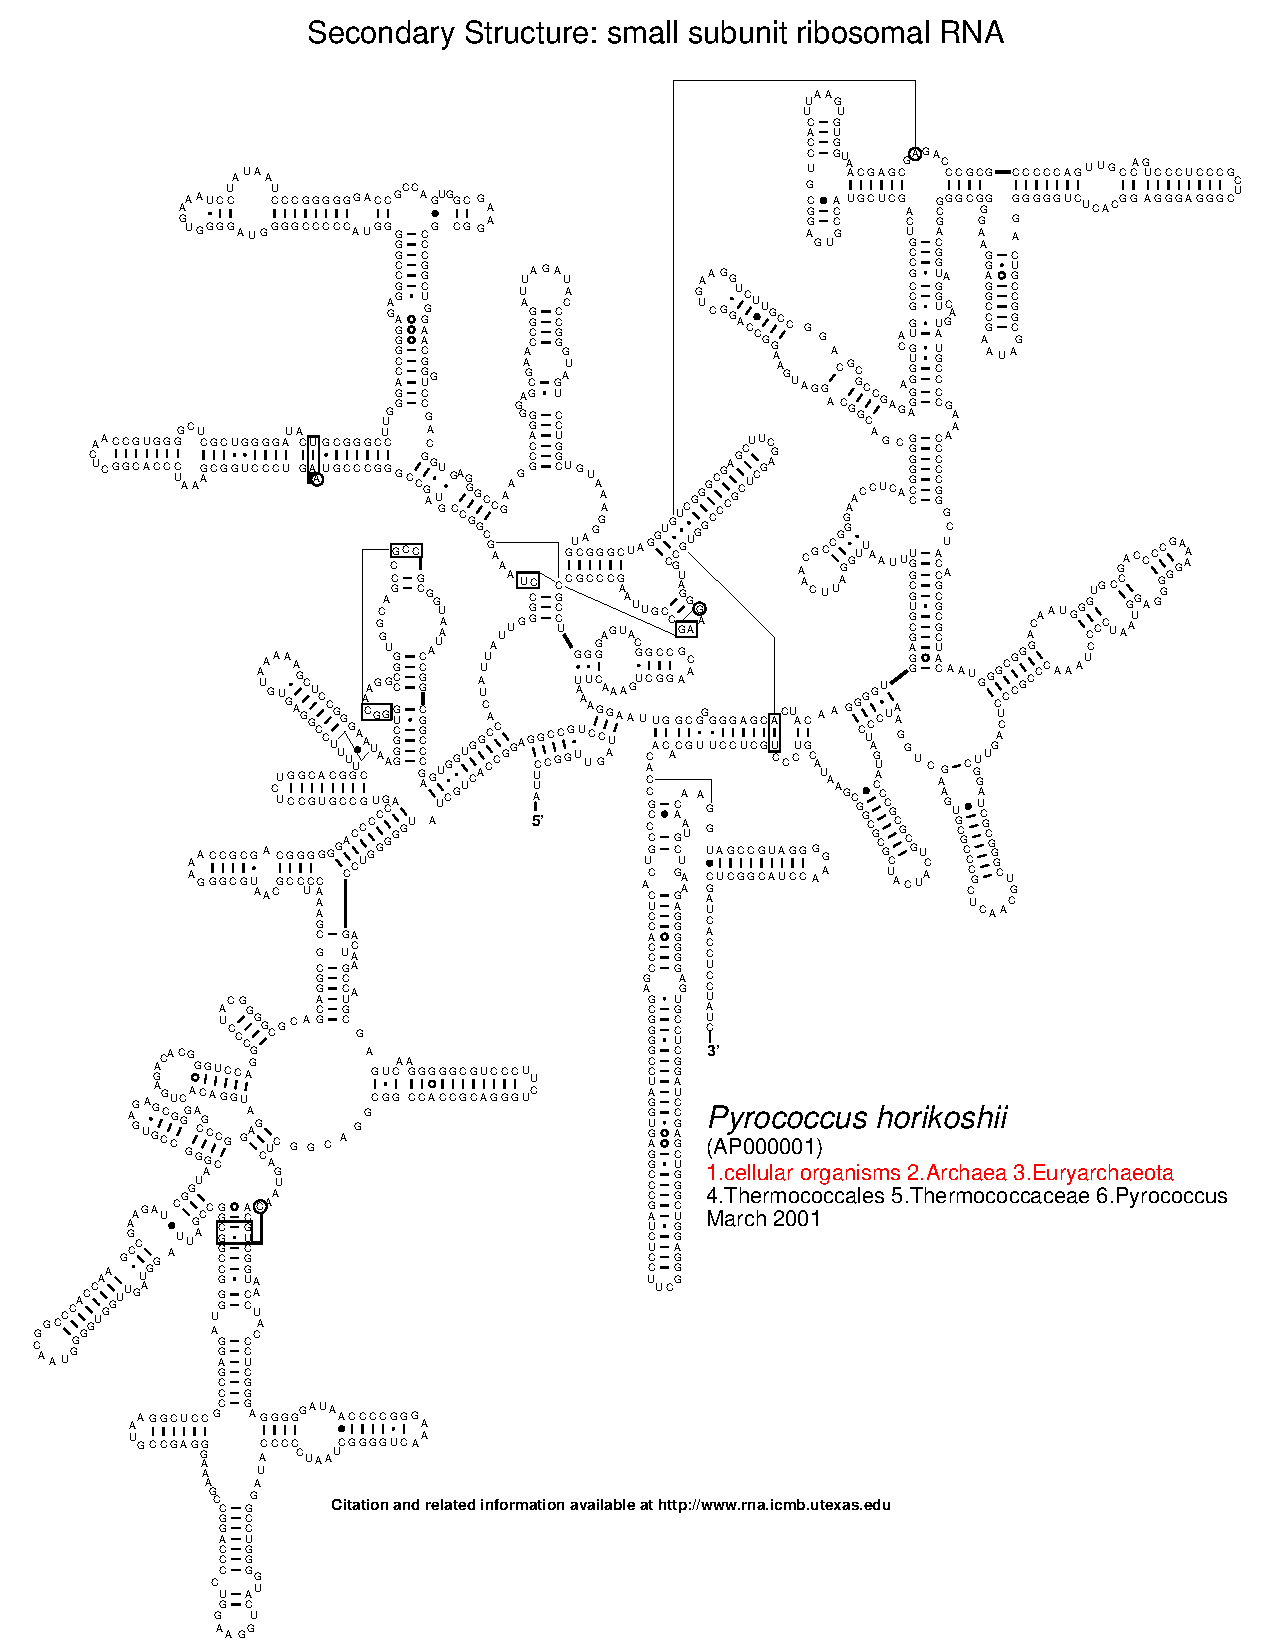
\includegraphics[height=8in]{figs/arc-17}\end{center}\vfill\end{slide}
%%%%%%%%%%%%%%%%%%%%%%%%%%%%%%%%%%%%%%%%%%%%%%%%%%%%%%%%%%%%%%%%%%%%%%%%%%%%%%%%%%%%%%%%%%%%%
\begin{slide}\begin{center}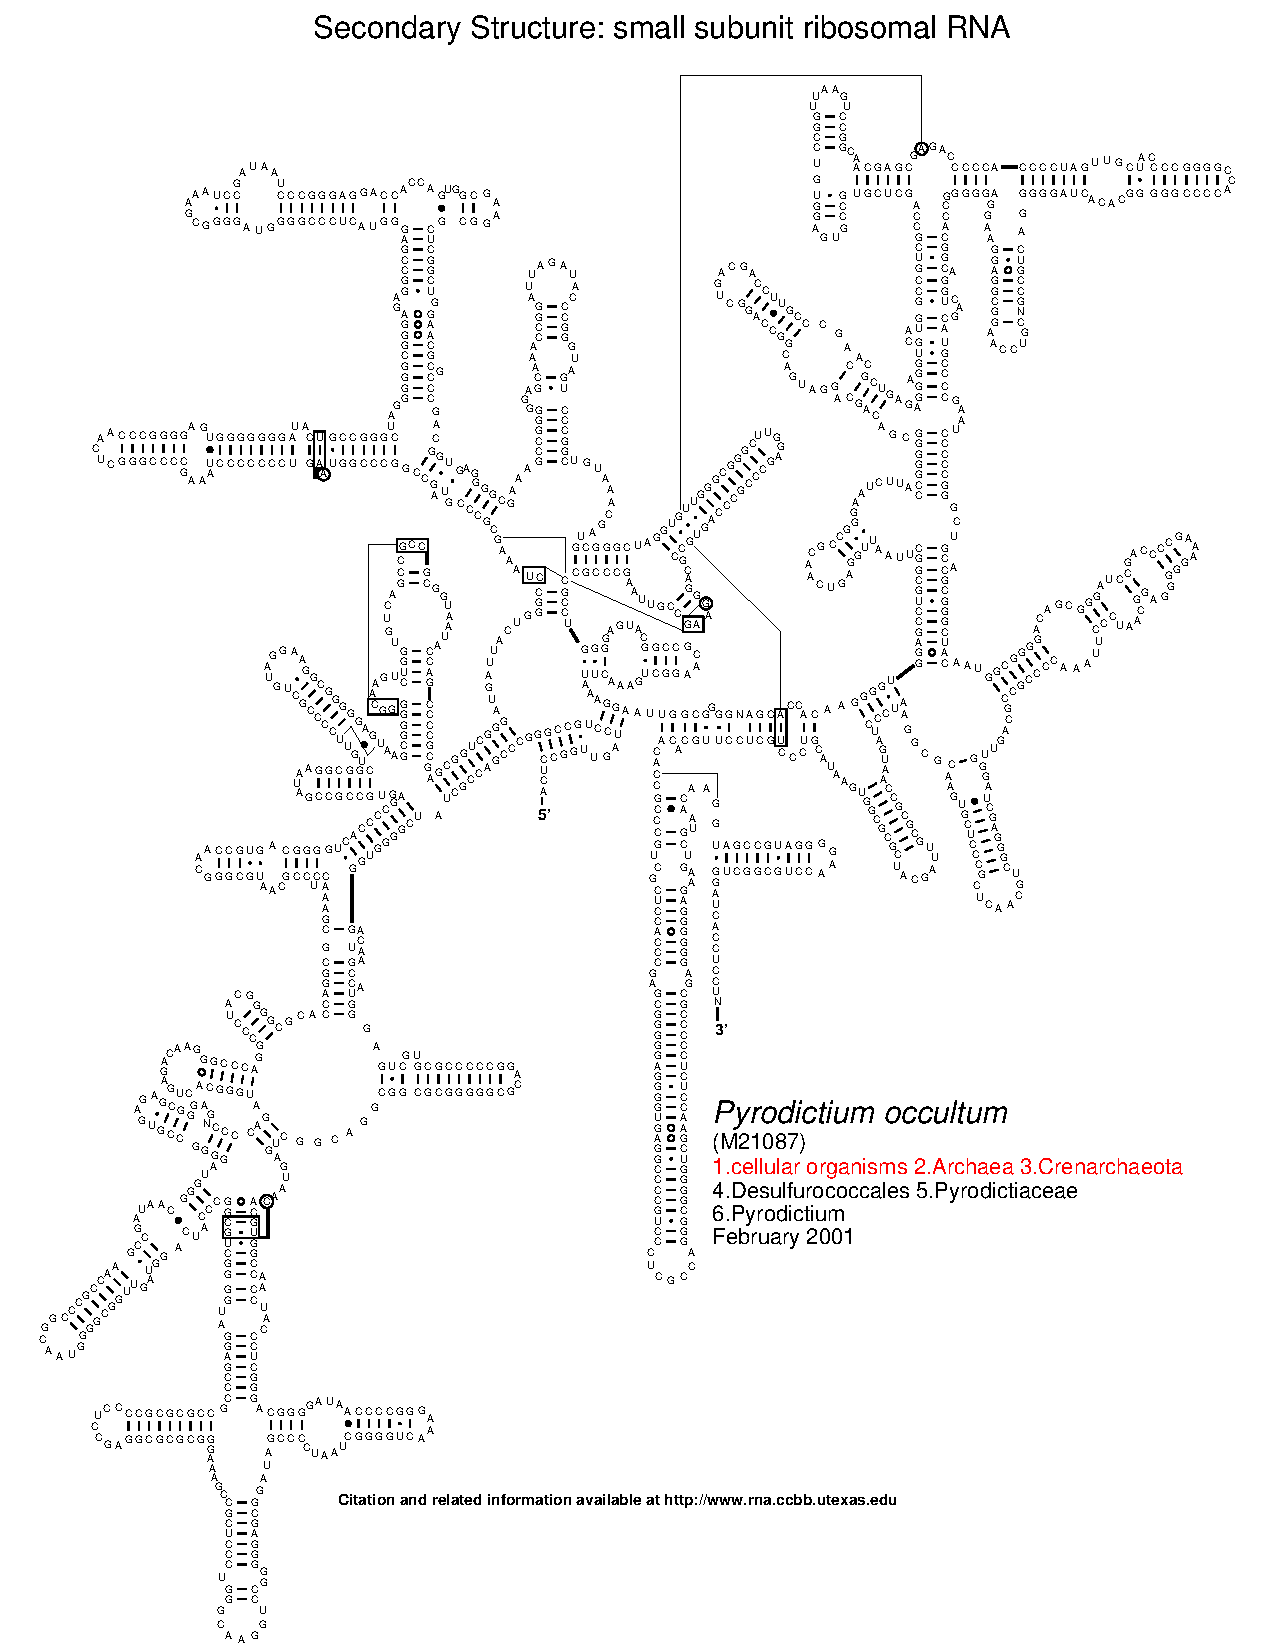
\includegraphics[height=8in]{figs/arc-18}\end{center}\vfill\end{slide}
%%%%%%%%%%%%%%%%%%%%%%%%%%%%%%%%%%%%%%%%%%%%%%%%%%%%%%%%%%%%%%%%%%%%%%%%%%%%%%%%%%%%%%%%%%%%%
\begin{slide}\begin{center}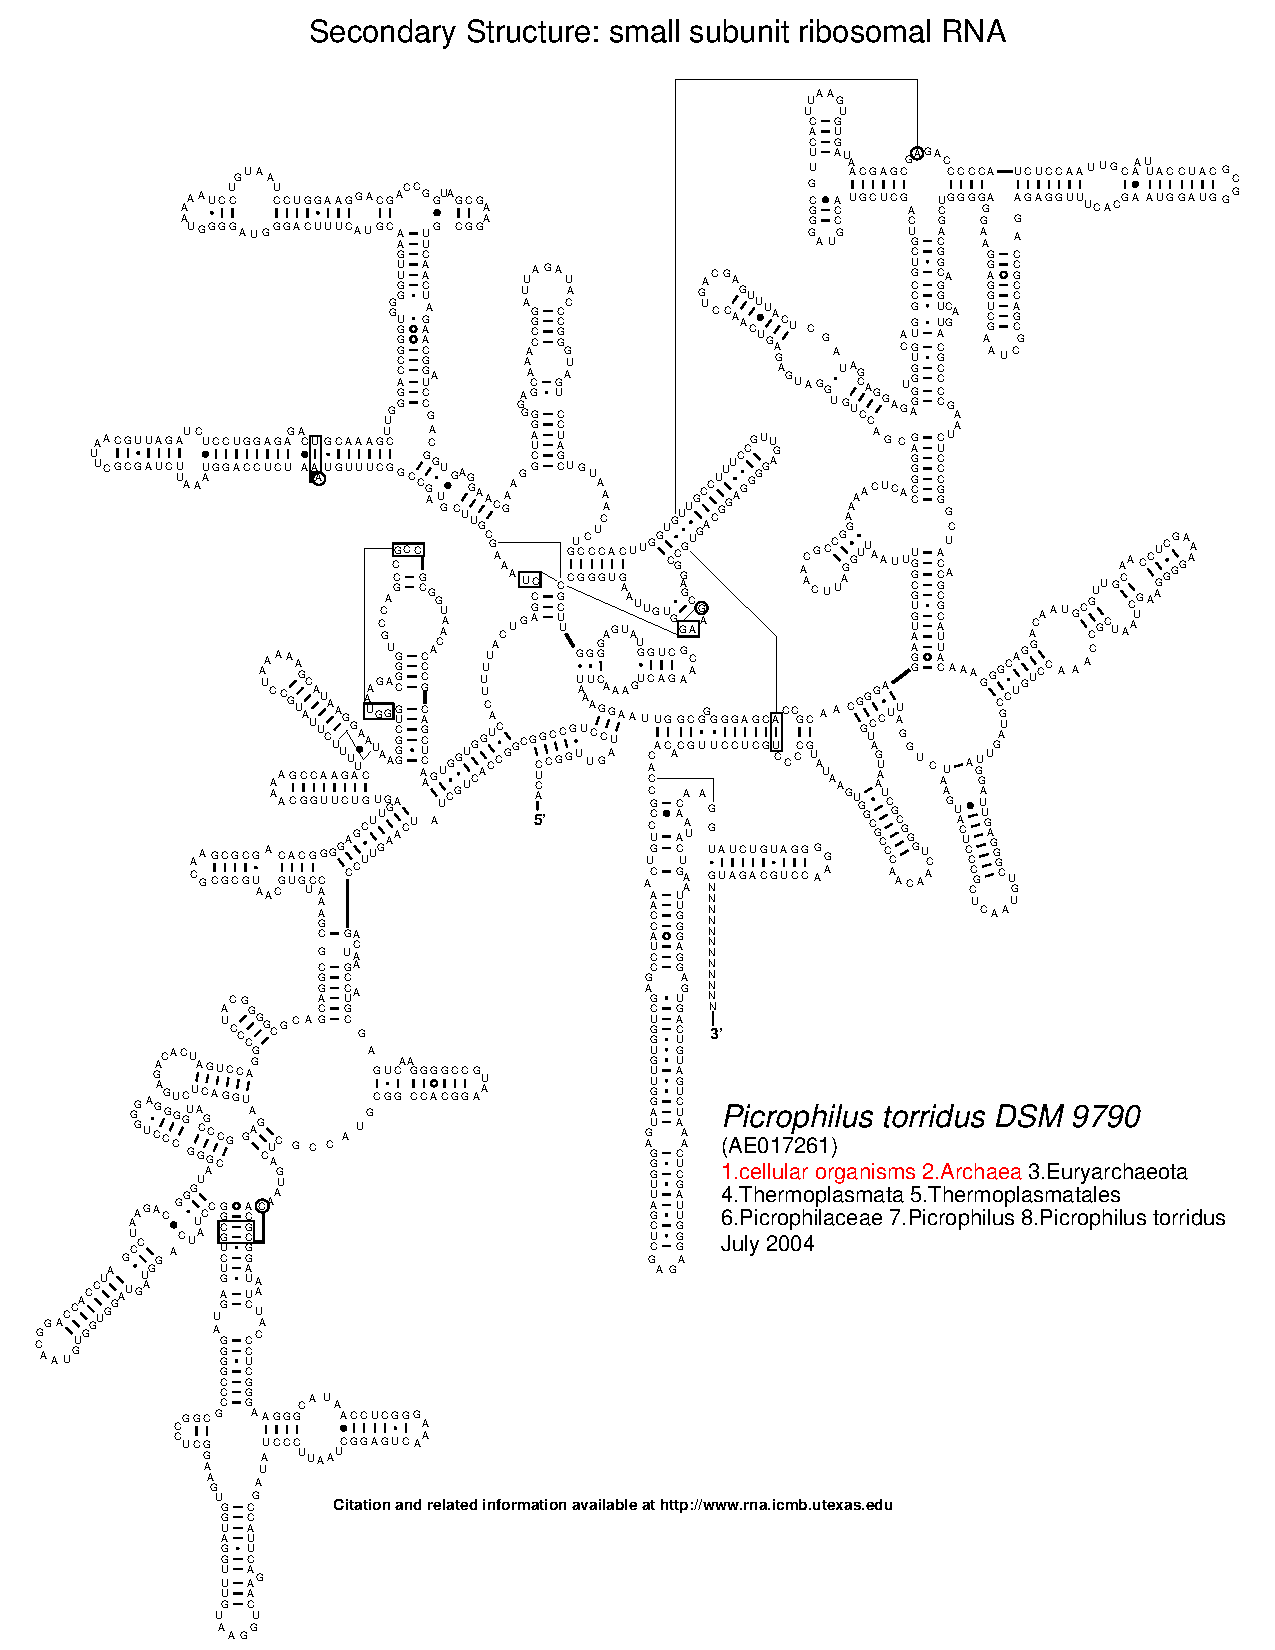
\includegraphics[height=8in]{figs/arc-19}\end{center}\vfill\end{slide}
%%%%%%%%%%%%%%%%%%%%%%%%%%%%%%%%%%%%%%%%%%%%%%%%%%%%%%%%%%%%%%%%%%%%%%%%%%%%%%%%%%%%%%%%%%%%%
%\begin{slide}\begin{center}\includegraphics[height=8in]{figs/arc-20}\end{center}\vfill\end{slide}
%%%%%%%%%%%%%%%%%%%%%%%%%%%%%%%%%%%%%%%%%%%%%%%%%%%%%%%%%%%%%%%%%%%%%%%%%%%%%%%%%%%%%%%%%%%%%
%\begin{slide}\begin{center}\includegraphics[height=8in]{figs/arc-21}\end{center}\vfill\end{slide}
%%%%%%%%%%%%%%%%%%%%%%%%%%%%%%%%%%%%%%%%%%%%%%%%%%%%%%%%%%%%%%%%%%%%%%%%%%%%%%%%%%%%%%%%%%%%%
\begin{slide}\begin{center}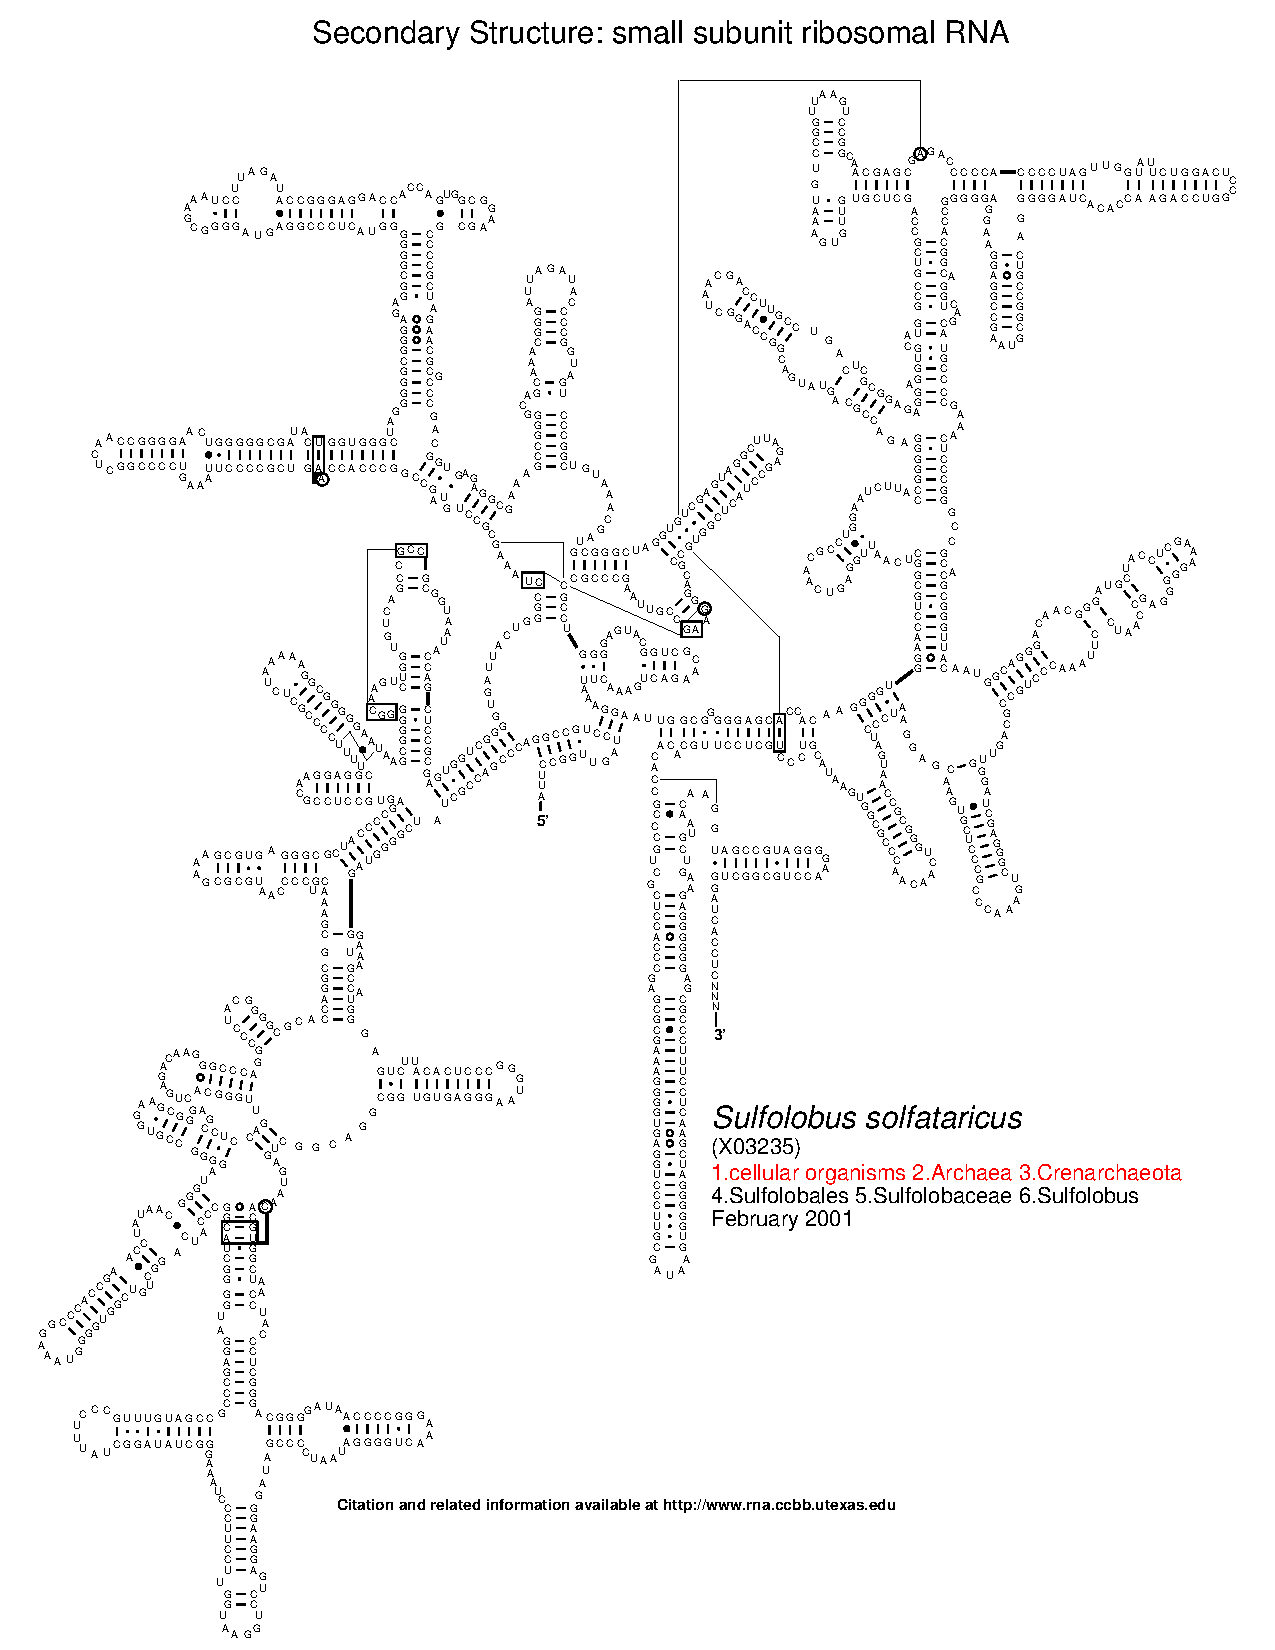
\includegraphics[height=8in]{figs/arc-22}\end{center}\vfill\end{slide}
%%%%%%%%%%%%%%%%%%%%%%%%%%%%%%%%%%%%%%%%%%%%%%%%%%%%%%%%%%%%%%%%%%%%%%%%%%%%%%%%%%%%%%%%%%%%%
\begin{slide}\begin{center}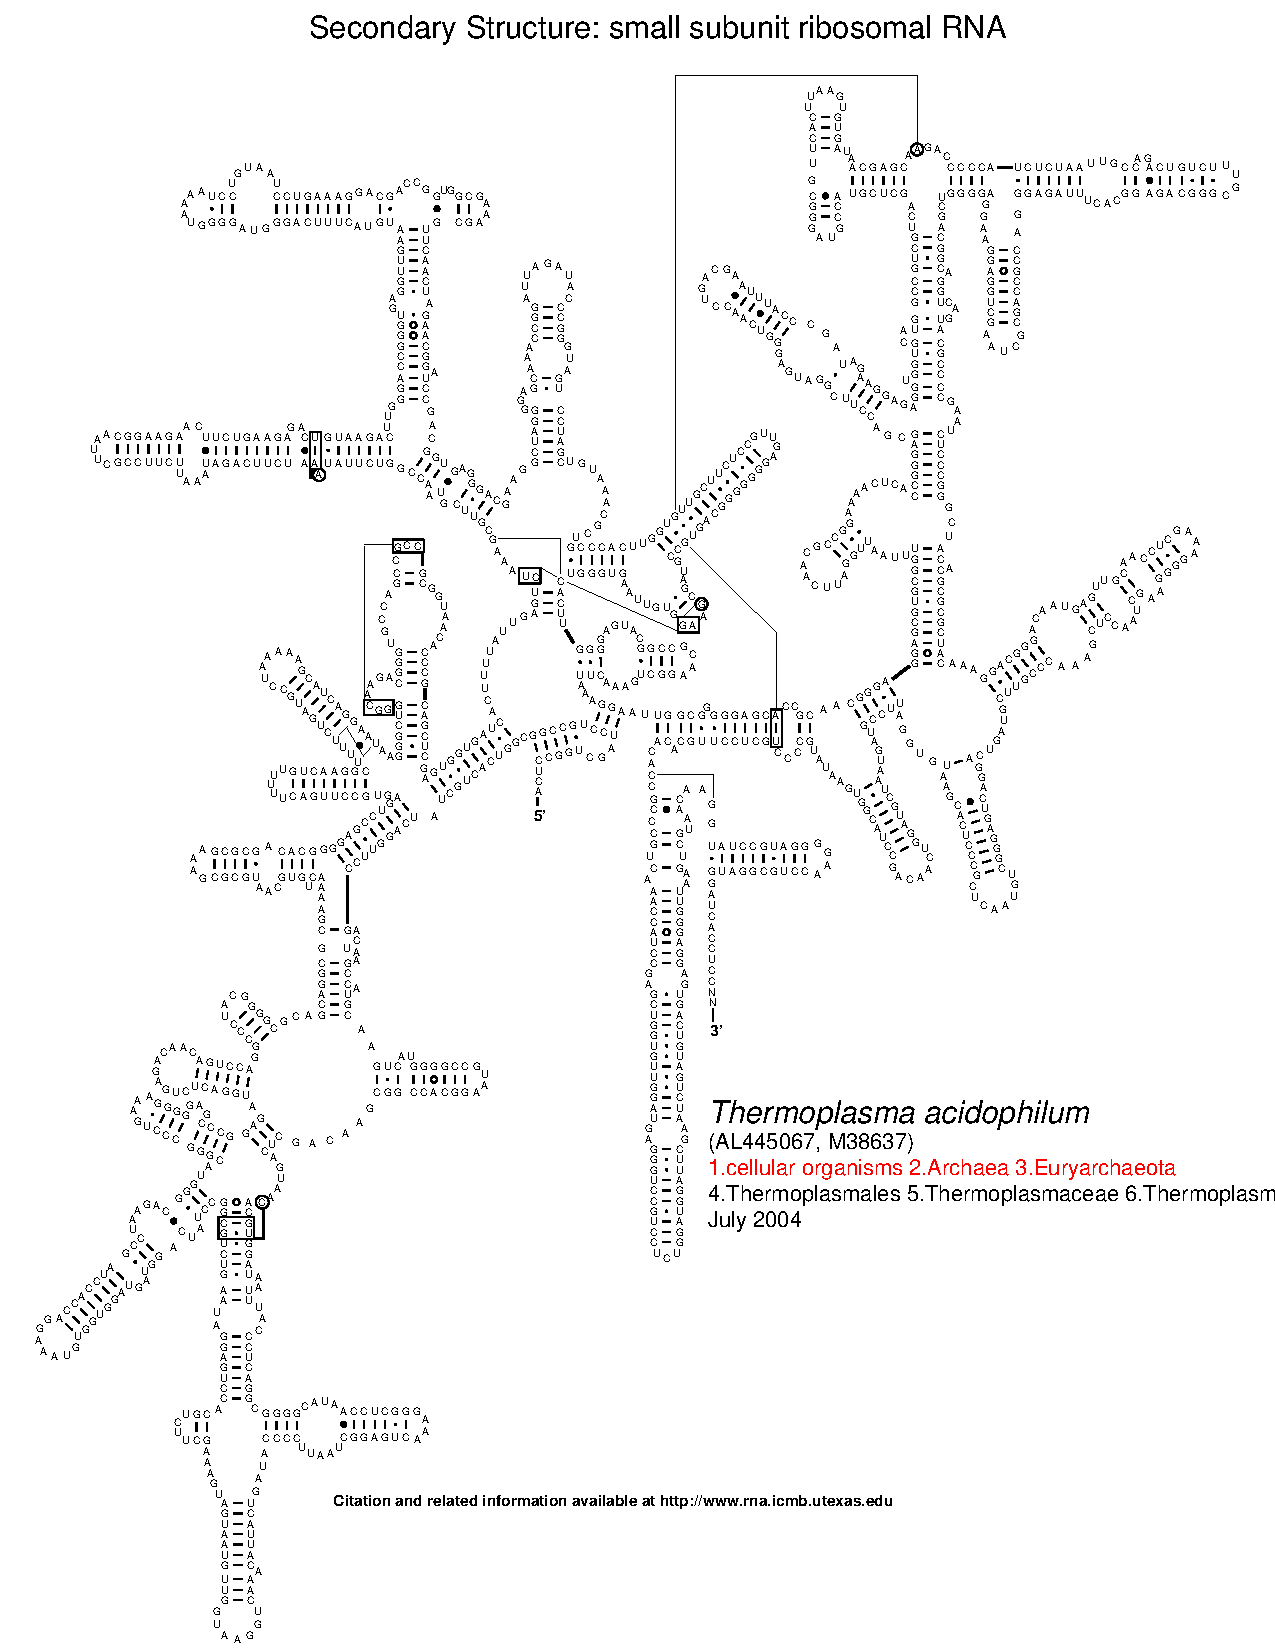
\includegraphics[height=8in]{figs/arc-23}\end{center}\vfill\end{slide}
%%%%%%%%%%%%%%%%%%%%%%%%%%%%%%%%%%%%%%%%%%%%%%%%%%%%%%%%%%%%%%%%%%%%%%%%%%%%%%%%%%%%%%%%%%%%%
\begin{slide}\begin{center}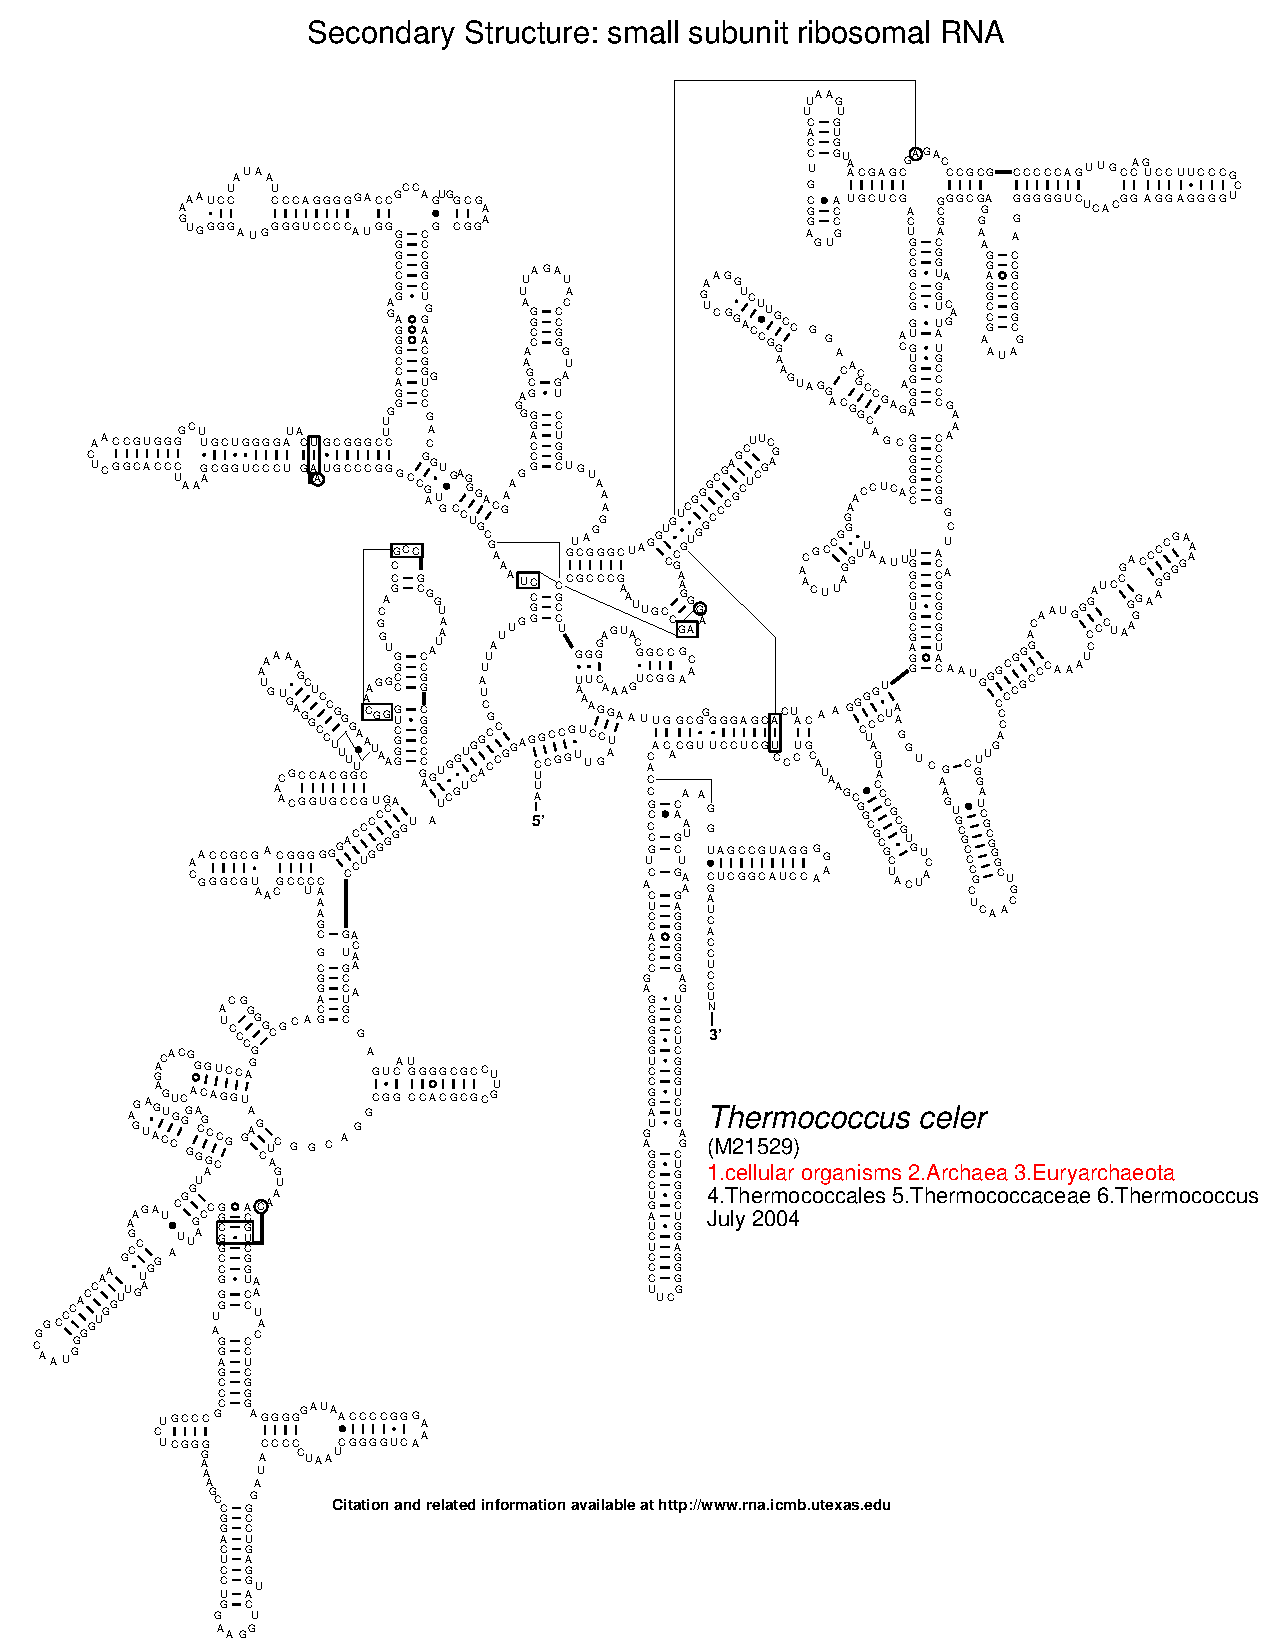
\includegraphics[height=8in]{figs/arc-24}\end{center}\vfill\end{slide}
%%%%%%%%%%%%%%%%%%%%%%%%%%%%%%%%%%%%%%%%%%%%%%%%%%%%%%%%%%%%%%%%%%%%%%%%%%%%%%%%%%%%%%%%%%%%%
\begin{slide}\begin{center}\includegraphics[height=8in]{figs/arc-25}\end{center}\vfill\end{slide}
%%%%%%%%%%%%%%%%%%%%%%%%%%%%%%%%%%%%%%%%%%%%%%%%%%%%%%%%%%%%%%%%%%%%%%%%%%%%%%%%%%%%%%%%%%%%%
\begin{slide}
%\begin{center}
%\textbf{Phil Hugenholtz's manually created mask}
%\end{center}
%\small
\begin{center}
\includegraphics[height=8in]{figs/archaea-mask-ph-only}
\end{center}
\vfill
\end{slide}
%%%%%%%%%%%%%%%%%%%%%%%%%%%%%%%%%%%%%%%%%%%%%%%%%%%%%%%%%%%%%%%%%%%%%%%%%%%%%%%%%%%%%%%%%%%%%
\begin{slide}
%\begin{center}
%\textbf{Automatically generated Archaeal mask using CM posterior probabilities}
%\end{center}
%\small
\begin{center}
\includegraphics[height=8in]{figs/archaea-mask-pp-only}
\end{center}
\vfill
\end{slide}
%%%%%%%%%%%%%%%%%%%%%%%%%%%%%%%%%%%%%%%%%%%%%%%%%%%%%%%%%%%%%%%%%%%%%%%%%%%%%%%%%%%%%%%%%%%%%
%%%%%%%%%%%%%%%%%%%%%%%%%%%%%%%%%%%%%%%%%%%%%%%%%%%%%%%%%%%%%%%%%%%%%%%%%%%%%%%%%%%%%%%%%%%%%
\begin{slide}
%\begin{center}
%\textbf{The manually created mask and automated CM-baseda mask are similar}
%\end{center}
%\small
\begin{center}
\includegraphics[width=10.5in]{figs/archaea-mask-ph-v-pp-both}
\end{center}
\vfill
\end{slide}
%%%%%%%%%%%%%%%%%%%%%%%%%%%%%%%%%%%%%%%%%%%%%%%%%%%%%%%%%%%%%%%%%%%%%%%%%%%%%%%%%%%%%%%%%%%%%
%%%%%%%%%%%%%%%%%%%%%%%%%%%%%%%%%%%%%%%%%%%%%%%%%%%%%%%%%%%%%%%%%%%%%%%%%%%%%%%%%%%%%%%%%%%%%
\begin{slide}
%\begin{center}
%\textbf{The manually created mask and automated CM-baseda mask are similar}
%\end{center}
%\small
\begin{center}
\includegraphics[height=8in]{figs/archaea-mask-ph-v-pp-diff}
\end{center}
\vfill
\end{slide}
%%%%%%%%%%%%%%%%%%%%%%%%%%%%%%%%%%%%%%%%%%%%%%%%%%%%%%%%%%%%%%%%%%%%%%%%%%%%%%%%%%%%%%%%%%%%%
%%%%%%%%%%%%%%%%%%%%%%%%%%%%%%%%%%%%%%%%%%%%%%%%%%%%%%%%%%%%%%%%%%%%%%%%%%%%%%%%%%%%%%%%%%%%%
%%%%%%%%%%%%%%%%%%%%%%%%%%%%%%%%%%%%%%%%%%%%%%%%%%%%%%%%%%%%%%%%%%%%%%%%%%%%%%%%%%%%%%%%%%%%%
\begin{slide}
%\begin{center}
%\textbf{The manually created mask and automated CM-baseda mask are similar}
%\end{center}
%\small
\begin{center}
\includegraphics[width=10.5in]{figs/archaea-mask-pp-and-deletes}
\end{center}
\vfill
\end{slide}
%%%%%%%%%%%%%%%%%%%%%%%%%%%%%%%%%%%%%%%%%%%%%%%%%%%%%%%%%%%%%%%%%%%%%%%%%%%%%%%%%%%%%%%%%%%%%
%%%%%%%%%%%%%%%%%%%%%%%%%%%%%%%%%%%%%%%%%%%%%%%%%%%%%%%%%
%%%%%%%%%%%%%%%%%%%%%%%%%%%%%%%%%%%%%%%%%%%%%%%%%%%%%%%%%
%%%%%%%%%%%%%%%%%%%%%%%%%%%%%%%%%%%%%%%%%%%%%%%%%%%%%%%%%%%%%%%%%%%%%%%%%%
\begin{slide}
\begin{center}

\textbf{Automated masking removes the majority of alignment errors}
\end{center}
\medskip
\medskip
\begin{center}

\begin{tabular}{rcr} 
& \multicolumn{1}{c}{alignment} & \multicolumn{1}{c}{time} \\
& \multicolumn{1}{c}{accuracy} & \multicolumn{1}{c}{(sec/seq)} \\ \hline
& \multicolumn{1}{c}{} & \multicolumn{1}{c}{} \\
Muscle-3.8.31\footnote{Edgar, R.C. Nucleic Acids Res 32(5), 1792-97.} & 95.4\% & 0.49 \\ 
& \multicolumn{1}{c}{} & \multicolumn{1}{c}{} \\
HMMER3 (HMMs) & 96.8\% & 0.04 \\ 
& \multicolumn{1}{c}{} & \multicolumn{1}{c}{} \\
Infernal 1.1 (CMs) & 98.1\% & 0.50 \\
& \multicolumn{1}{c}{} & \multicolumn{1}{c}{} \\
\textcolor{red}{Infernal 1.1 (CMs)} & & \\
\textcolor{red}{posterior probability masked} & \textcolor{red}{99.5\%} & \textcolor{red}{0.50} \\ %1.1
\textcolor{red}{(1302/1530 columns)} & & \\
\end{tabular}
\end{center}

\center{
{\bf Infernal produces alignment that are \\ very similar to manually
  refined alignments.}}

\vfill
\end{slide}
%%%%%%%%%%%%%%%%%%%%%%%%%%%%%%%%%%%%%%%%%%%%%%%%%%%%%%%%%%%%%%%%%%%%%%%%%%
\begin{slide}
\begin{center}
\textbf{SSU-ALIGN: structural alignment of SSU rRNAs using CMs}
\end{center}

\includegraphics[width=10in]{figs/seq2tree-2013-ssu-align}

\vfill
\end{slide}
%%%%%%%%%%%%%%%%%%%%%%%%%%%%%%%%%%%%%%%%%%%%%%%%%%%%%%%%%%%%%%%%%%%%
\begin{slide}

\large
\begin{center}
\large{\textbf{Acknowledgements}} \\

\vspace{0.5in}

\normalsize
%\begin{tabular}{llllll}
%Sean Eddy           & & & & & Michael Brent \\ 
%Elena Rivas         & & & & & Jeremy Buhler \\
%Tom Jones           & & & & & Justin Fay \\
%Diana Kolbe         & & & & & Jeff Gordon \\
%Seolkyoung Jung     & & & & & Rob Mitra \\
%Sergi Castellano    & & & & & Gary Stormo \\
%Fred Davis          & & & & & \\
%Lee Henry           & & & & & \\
%Michael Farrar      & & & & & \\
%Travis Wheeler      & & & & & \\
\begin{tabular}{l}
Sean Eddy           \\
Elena Rivas         \\
Travis Wheeler      \\
Tom Jones           \\
Diana Kolbe         \\
Seolkyoung Jung     \\
Rob Finn            \\
Jody Clements       \\
Fred Davis          \\
Lee Henry           \\
Michael Farrar      \\
\end{tabular}

\includegraphics[height=3in]{figs/jfrc-banner1}

\end{center}

\vfill
\end{slide}
%%%%%%%%%%%%%%%%%%%%%%%%%%%%%%%%%%%%%%%%%%%%%%%%%%%%%%%%%%%%%%%
\end{document}

